\documentclass{article}

% Add this code and Bib.bib
\usepackage[english]{babel}
\usepackage[autostyle]{csquotes}
\usepackage[backend=biber,style=authoryear]{biblatex}
\usepackage{changepage}
\usepackage{minted}
\addbibresource{Bib.bib}
\usepackage{graphicx}
\usepackage{amsmath}
\usepackage[parfill]{parskip}
\usepackage[bottom]{footmisc} % push footnotes at the end when pagebreak
% Accent on rds name
\usepackage[utf8]{inputenc}
\usepackage{enumitem} % enumarate

\addtolength{\oddsidemargin}{-.875in}
\addtolength{\evensidemargin}{-.875in}
\addtolength{\textwidth}{1.75in}
\addtolength{\topmargin}{-.875in}
\addtolength{\textheight}{1.75in}


\title{Big Data Final Project}
\author {Eduardo Fierro (eff254), Akash Kadel (ak6201), Raúl Delgado (rds491)}

\begin{document}
\maketitle
\begin{center}
Github-Repo URL: https://github.com/edufierro/BigDataProject
\end{center}

\bigskip
\bigskip


\begin{center}
\textbf{Abstract}
\end{center}
\bigskip

In this report, we analyze the quality of the Crime data updated by the City of New York. This data contains over 5.58 million rows and 24 different features. First, we comment on the temporality of the Data, noting several problems on the year and hour of the time of occurrence, and some minor problems regarding the categorization. Next, we analyzed 6 different hypothesis in two main topics: Sociodemographic characteristics of population and Baseball Games. We found evidence that more population, more black population as percent of total population, more population below poverty line and less educated population as percentage of total population is highly correlated with an increase in crime at any given Borough in any given year. We also found that crime increases on Baseball Game - day near the stadium in that particular day, and this is even more clear near the Citi Field stadium compared with the Yankee Stadium. 

\pagebreak
\tableofcontents
\pagebreak

\section{Introduction}

Crime in New York City, as in many megalopolis around the world, has been a longstanding issue. Nonetheless, in recent years, according to the Bureau of Justice Statistics, crime in New York has never seen a drop in the homicide rate and criminal actions in general ~\autocite{drop_in_Crime1}.  

This drop in crimes came hand in hand with the liberation of vast amounts of data from the City of New York, which includes the liberation of geocoded crime data, including over 5.4 million crimes described by 24 features. Nevertheless, as any data frame this big, it has some inherent problems. 

On the second section of this report, we analyzed thoroughly the data-frame, downloaded directly form the NY City Open Data Portal\footnote{The data can be downloaded from: https://data.cityofnewyork.us/Public-Safety/NYPD-Complaint-Data-Historic/qgea-i56i}. We found that the data frame has many problems when it comes to temporarily: Most of the data is reliable for crimes committed after 2006. We also found that the time encoding for the time of occurrence of the crime is usually rounded to the nearest hour, or even to noon when there is no specified time when the crime was committed. Last, we recommend the institution responsible for the Data (in this case, the data is provided to the portal by the Police Department (NYPD)), to generate an external codebook for the crime categories keys and description, since the it is not clear in the data which keys correspond to which crimes.

Next, we decided to test 2 different ``families'' of hypothesis: A macro-level set of hypothesis and a micro-level set. For the macro level, we tested 4 different hypothesis aggregated at a borough-year level: 
\begin{itemize}
\item An increase in population is correlated with an increase in the number of crimes.
\item Crime is positively correlated with the percentage of black population among total population. 
\item There is also a positive correlation between the percentage of people in the borough with no other studies that high-school and crime. 
\item There is a strong and positive correlation between the percentage of people living under poverty line and crime
\end{itemize}
All of these hypothesis turned out to be true for New York. At a more specific borough-level analysis, the only one of the 5 boroughs that differs from the rest is Staten Island. 

On the micro-level side of the analysis, we decided to explore how sport events affect the occurrence of crimes around the sport venue. Because of the amount of data available for each sport, we decided to analyze solely Baseball, with the following hypothesis: 
\begin{itemize}
\item A baseball game increases the occurrence of crime around a Baseball stadium at the day of the event. 
\item If so, there is a clear difference between Citi Field (Mets) and Yankee Stadium. 
\end{itemize}
To perform this analysis, we subset the data to only those crimes around 4 different bounding boxes around the stadium: 250 meters, 500 meters, 1000 meters and 2000 meters. After this, we aggregated the data in days, and analyzed the mean difference in daily crimes when there is no game compared to when there is a game. 

We conclude that there is a clear trend when we analyzed all the crimes together at any of the distances above specified. For example, a baseball game increases in 13 crimes on average the compared to days when there is no baseball games at a 2000 meters bounding box around Yankee Stadium. Nonetheless, when we analyzed specific crimes, only a few appear to be statistically different when there is a Baseball game compared to when there is no Baseball game. 

After this two sections, a summary of the report and the main conclusions are drawn. 

\pagebreak
\section{Part I: NYC Crime Data Issues and Summary}
\subsection{Basic analysis on valid entries}

Our first approach to a Data Frame as big as the Data Frame uploaded by the New York City Police Department was to make a basic description and validation assessment per column. It's worth mentioning, as part of the basic description of the data frame, that this table contains, not including the header/column names, 5,101,231 rows and 24 rows. 

The main findings of this section include the fact that the dates seem not to be very consistent with reality, and further and further analysis on them needs to be made. We also conclude that there are string inconsistencies with the classification codes for the crime: Mainly, we would recommend to keep an external codebook for \texttt{KY\_CD}, so the variable and it's description can be evaluated externally and not endogenously.  We also saw some discrepancies between the \texttt{PARKS\_NM} and  \texttt{HADEVELOPT} and the \texttt{PREM\_TYP\_DESC} variables: Mainly, when \texttt{PARKS\_NM} and  \texttt{HADEVELOPT} are not NULL, \texttt{PREM\_TYP\_DESC} doesn't take uniquely the value of "PARK/PLAYGROUND" or "RESIDENCE - PUBLIC HOUSING". 

\begin{itemize}
\item CMPLNT\_NUM: \\
The first column in the data-frame refers to an ID for each row on tha data. To asses the validity of this column, the most obvious approach is to asses if the column is unique for all rows. This can be done counting the unique values of the column and counting the all the values for the column. 

\begin{minted}{python}
+--------------------------+                                             
|count(DISTINCT CMPLNT_NUM)|
+--------------------------+
|                   5101231|
+--------------------------+

+-----------------+                                                     
|count(CMPLNT_NUM)|
+-----------------+
|          5101231|
+-----------------+
\end{minted}

Once we proved it was unique, a validity criterion then was defined for each value: If the id lies between 100,000,000 and  999,999,999, and if not null, then we considered it a valid ID. It turned out that all the values/rows for this column were valid: 

\begin{minted}{python}
+----------+---------+-----------------+--------+
|CMPLNT_NUM|base_type|    semantic_type|is_valid|
+----------+---------+-----------------+--------+
| 101109527|  integer|commplaint number|   valid|
| 153401121|  integer|commplaint number|   valid|
| 569369778|  integer|commplaint number|   valid|
| 968417082|  integer|commplaint number|   valid|
| 641637920|  integer|commplaint number|   valid|
| 365661343|  integer|commplaint number|   valid|
| 608231454|  integer|commplaint number|   valid|
| 265023856|  integer|commplaint number|   valid|
| 989238731|  integer|commplaint number|   valid|
| 415095955|  integer|commplaint number|   valid|
| 731283092|  integer|commplaint number|   valid|
| 178090167|  integer|commplaint number|   valid|
| 898496564|  integer|commplaint number|   valid|
| 566081066|  integer|commplaint number|   valid|
| 584555879|  integer|commplaint number|   valid|
| 715942154|  integer|commplaint number|   valid|
| 338440707|  integer|commplaint number|   valid|
| 433257334|  integer|commplaint number|   valid|
| 761004485|  integer|commplaint number|   valid|
| 234892198|  integer|commplaint number|   valid|
+----------+---------+-----------------+--------+
only showing top 20 rows

+--------+---------------+                                            
|is_valid|count(is_valid)|
+--------+---------------+
|   valid|        5101231|
+--------+---------------+
\end{minted}

\item CMPLNT\_FR\_DT: \\
According to the description available in the NYC Open Data web page, this column refers to the "Exact date of occurrence for the reported event (or starting date of occurrence, if CMPLNT\_TO\_DT exists)". 

Our first step to assess this column was to check the min and max value for each year, along with the unique years in the data frame. It's worth remembering that this section only addresses the issue regarding the validity of the data, not the credibility of it. For now, we are only checking that the data has a certain shape and type, not if this makes sense. This second issue will be deeply described in the next section.  

\begin{minted}{python}
+-----------------------------+ 
|substring(CMPLNT_FR_DT, 7, 4)|
+-----------------------------+
|                         1987|
|                         1956|
|                         2012|
|                         1958|
|                         1910|
|                         1915|
|                         1972|
|                         1911|
|                         1988|
|                         1938|
|                         1977|
|                         1971|
|                         2014|
|                         1984|
|                         1982|
|                         2013|
|                         1941|
|                         2005|
|                         1919|
|                         2000|
+-----------------------------+
only showing top 20 rows
\end{minted}
\pagebreak
\begin{minted}{python}
+----------------------------------------------------------------------+   
|min(CAST(CAST(substring(CMPLNT_FR_DT, 7, 4) AS DECIMAL(20,0)) AS INT))|
+----------------------------------------------------------------------+
|                                                                  1015|
+----------------------------------------------------------------------+


+----------------------------------------------------------------------+   
|max(CAST(CAST(substring(CMPLNT_FR_DT, 7, 4) AS DECIMAL(20,0)) AS INT))|
+----------------------------------------------------------------------+
|                                                                  2015|
+----------------------------------------------------------------------+
\end{minted}

As seen above, the minimum year is 1015, and the maximum year is 2015. To further asses the validity of the data, a filter for validity was defined in the following way: Check if the year (all string after the last slash) was greater than 1900, check if month (string between the two slashes) is something between 1 and 12, and day (string before the first slash) is between 1 and 31. 

\begin{minted}{python}
+------------+---------+------------------+--------+
|CMPLNT_FR_DT|base_type|     semantic_type|is_valid|
+------------+---------+------------------+--------+
|  12/31/2015|timestamp|date of occurrence|   valid|
|  12/31/2015|timestamp|date of occurrence|   valid|
|  12/31/2015|timestamp|date of occurrence|   valid|
|  12/31/2015|timestamp|date of occurrence|   valid|
|  12/31/2015|timestamp|date of occurrence|   valid|
|  12/31/2015|timestamp|date of occurrence|   valid|
|  12/31/2015|timestamp|date of occurrence|   valid|
|  12/31/2015|timestamp|date of occurrence|   valid|
|  12/31/2015|timestamp|date of occurrence|   valid|
|  12/31/2015|timestamp|date of occurrence|   valid|
|  12/31/2015|timestamp|date of occurrence|   valid|
|  12/31/2015|timestamp|date of occurrence|   valid|
|  12/31/2015|timestamp|date of occurrence|   valid|
|  12/31/2015|timestamp|date of occurrence|   valid|
|  12/31/2015|timestamp|date of occurrence|   valid|
|  12/31/2015|timestamp|date of occurrence|   valid|
|  12/31/2015|timestamp|date of occurrence|   valid|
|  12/31/2015|timestamp|date of occurrence|   valid|
|  12/31/2015|timestamp|date of occurrence|   valid|
|  12/31/2015|timestamp|date of occurrence|   valid|
+------------+---------+------------------+--------+
only showing top 20 rows

+--------+---------------+                                               
|is_valid|count(is_valid)|
+--------+---------------+
|   valid|        5100564|
| invalid|             12|
|    null|            655|
+--------+---------------+
\end{minted}

Under this criterion, the data contains then 655 missing values for date, and 12 dates with invalid values. Again, this will be further analyzed in the next section. 

\item CMPLNT\_FR\_TM: \\
This third column represents, according to the data description, "Exact time of occurrence for the reported event (or starting time of occurrence, if CMPLNT\_TO\_TM exists)". After checking the format of the column, the validity criterion was defined in the following way: Hour has to be between 0 and 23, minute between 0 and 59 and seconds also between 0 and 59. 

\begin{minted}{python}
+------------+---------+------------------+--------+
|CMPLNT_FR_TM|base_type|     semantic_type|is_valid|
+------------+---------+------------------+--------+
|    23:45:00|timestamp|time of occurrence|   valid|
|    23:36:00|timestamp|time of occurrence|   valid|
|    23:30:00|timestamp|time of occurrence|   valid|
|    23:30:00|timestamp|time of occurrence|   valid|
|    23:25:00|timestamp|time of occurrence|   valid|
|    23:18:00|timestamp|time of occurrence|   valid|
|    23:15:00|timestamp|time of occurrence|   valid|
|    23:15:00|timestamp|time of occurrence|   valid|
|    23:15:00|timestamp|time of occurrence|   valid|
|    23:10:00|timestamp|time of occurrence|   valid|
|    23:05:00|timestamp|time of occurrence|   valid|
|    23:00:00|timestamp|time of occurrence|   valid|
|    23:00:00|timestamp|time of occurrence|   valid|
|    23:00:00|timestamp|time of occurrence|   valid|
|    23:00:00|timestamp|time of occurrence|   valid|
|    23:00:00|timestamp|time of occurrence|   valid|
|    23:00:00|timestamp|time of occurrence|   valid|
|    23:00:00|timestamp|time of occurrence|   valid|
|    23:00:00|timestamp|time of occurrence|   valid|
|    22:55:00|timestamp|time of occurrence|   valid|
+------------+---------+------------------+--------+
only showing top 20 rows

+--------+---------------+      
|is_valid|count(is_valid)|
+--------+---------------+
|   valid|        5100529|
| invalid|            654|
|    null|             48|
+--------+---------------+
\end{minted}

Of all the values, there are a total of 48 missing and 654 invalid under this criteria. Again, further analysis is going to be made on this column. 

\item CMPLNT\_TO\_DT: \\
This is, according to the description of the data frame, the "Ending date of occurrence for the reported event, if exact time of occurrence is unknown". For this column, given the similarity with \texttt{CMPLNT\_FR\_DT}, the same validity criterion was applied. 
\begin{minted}{python}
+------------+---------+--------------------+--------+
|CMPLNT_TO_DT|base_type|       semantic_type|is_valid|
+------------+---------+--------------------+--------+
|            |timestamp|ending date of oc...|    null|
|            |timestamp|ending date of oc...|    null|
|            |timestamp|ending date of oc...|    null|
|            |timestamp|ending date of oc...|    null|
|  12/31/2015|timestamp|ending date of oc...|   valid|
|  12/31/2015|timestamp|ending date of oc...|   valid|
|            |timestamp|ending date of oc...|    null|
|  12/31/2015|timestamp|ending date of oc...|   valid|
|  12/31/2015|timestamp|ending date of oc...|   valid|
|  12/31/2015|timestamp|ending date of oc...|   valid|
|  12/31/2015|timestamp|ending date of oc...|   valid|
|  12/31/2015|timestamp|ending date of oc...|   valid|
|            |timestamp|ending date of oc...|    null|
|            |timestamp|ending date of oc...|    null|
|            |timestamp|ending date of oc...|    null|
|  12/31/2015|timestamp|ending date of oc...|   valid|
|  12/31/2015|timestamp|ending date of oc...|   valid|
|  12/31/2015|timestamp|ending date of oc...|   valid|
|  12/31/2015|timestamp|ending date of oc...|   valid|
|  12/31/2015|timestamp|ending date of oc...|   valid|
+------------+---------+--------------------+--------+
only showing top 20 rows

+--------+---------------+
|is_valid|count(is_valid)|
+--------+---------------+
|   valid|        3709752|
| invalid|              1|
|    null|        1391478|
+--------+---------------+
\end{minted}

Incredibly, 49.99\% of the data is null for this observation (meaning it has no value for this column). There is only one invalid row for it under the validation criteria specified above. This gives us a clue of how useless this column can be to do any analysis, since it would mean to discard certain information, and perhaps falling in a self-selection bias (perhaps, for example, the crimes that have an ending date and time, refer to non-violent crimes). We could also assume that if null, end date is equal to begin date, but with no further explanation of the data frame, this may be a huge assumption (i.e. What if it is really NULL?).

\item CMPLNT\_TO\_TM: \\

This column is describes officially as "Ending time of occurrence for the reported event, if exact time of occurrence is unknown". As the case of the "end-date" column, the same validity criterion was followed as the column \texttt{CMPLNT\_FR\_TM}. The results are the following: 
\begin{minted}{python}
+------------+---------+--------------------+--------+
|CMPLNT_TO_TM|base_type|       semantic_type|is_valid|
+------------+---------+--------------------+--------+
|            |timestamp|ending time of oc...|    null|
|            |timestamp|ending time of oc...|    null|
|            |timestamp|ending time of oc...|    null|
|            |timestamp|ending time of oc...|    null|
|    23:30:00|timestamp|ending time of oc...|   valid|
|    23:25:00|timestamp|ending time of oc...|   valid|
|            |timestamp|ending time of oc...|    null|
|    23:15:00|timestamp|ending time of oc...|   valid|
|    23:30:00|timestamp|ending time of oc...|   valid|
|    23:10:00|timestamp|ending time of oc...|   valid|
|    23:15:00|timestamp|ending time of oc...|   valid|
|    23:05:00|timestamp|ending time of oc...|   valid|
|            |timestamp|ending time of oc...|    null|
|            |timestamp|ending time of oc...|    null|
|            |timestamp|ending time of oc...|    null|
|    23:05:00|timestamp|ending time of oc...|   valid|
|    23:10:00|timestamp|ending time of oc...|   valid|
|    23:05:00|timestamp|ending time of oc...|   valid|
|    23:05:00|timestamp|ending time of oc...|   valid|
|    23:10:00|timestamp|ending time of oc...|   valid|
+------------+---------+--------------------+--------+
only showing top 20 rows

+--------+---------------+
|is_valid|count(is_valid)|
+--------+---------------+
|   valid|        3712070|
| invalid|           1376|
|    null|        1387785|
+--------+---------------+
\end{minted}

In this case, 27,2\% of the data has a missing. This might give us a clue of the true value of missing values for date. But it also sheds light on how useless it would be to use this couple of columns: Can we really measure how long it takes to murder someone with the data? Does this column reflects when the police took notice of the crime or the time in minutes it took to be committed? 

\item RPT\_DT: \\
This column, meaning "Date event was reported to police" has the same date format as \texttt{CMPLNT\_FR\_DT} and \texttt{CMPLNT\_TO\_DT}. Naturally, the same validity criteria was applied. The results show that all of these values are valid and non-missing. 

\begin{minted}{python}
+----------+---------+---------------+--------+
|    RPT_DT|base_type|  semantic_type|is_valid|
+----------+---------+---------------+--------+
|12/31/2015|timestamp|date of report |   valid|
|12/31/2015|timestamp|date of report |   valid|
|12/31/2015|timestamp|date of report |   valid|
|12/31/2015|timestamp|date of report |   valid|
|12/31/2015|timestamp|date of report |   valid|
|12/31/2015|timestamp|date of report |   valid|
|12/31/2015|timestamp|date of report |   valid|
|12/31/2015|timestamp|date of report |   valid|
|12/31/2015|timestamp|date of report |   valid|
|12/31/2015|timestamp|date of report |   valid|
|12/31/2015|timestamp|date of report |   valid|
|12/31/2015|timestamp|date of report |   valid|
|12/31/2015|timestamp|date of report |   valid|
|12/31/2015|timestamp|date of report |   valid|
|12/31/2015|timestamp|date of report |   valid|
|12/31/2015|timestamp|date of report |   valid|
|12/31/2015|timestamp|date of report |   valid|
|12/31/2015|timestamp|date of report |   valid|
|12/31/2015|timestamp|date of report |   valid|
|12/31/2015|timestamp|date of report |   valid|
+----------+---------+---------------+--------+
only showing top 20 rows

+--------+---------------+
|is_valid|count(is_valid)|
+--------+---------------+
|   valid|        5101231|
+--------+---------------+
\end{minted}

\item KY\_CD: \\
This column represents the "Three digit offense classification code" of the crime. As a first approach, we decided to take the minimum and the maximum value, particularly to make sure no "000" or "999" values were on the data, values usually encoded to indicate missing-values. This did not seem to be the case. 

\begin{minted}{python}
+----------+
|min(KY_CD)|
+----------+
|       101|
+----------+

+----------+
|max(KY_CD)|
+----------+
|       881|
+----------+
\end{minted}

After this, a selection criteria was defined: Existing values that when transformed to integer lie between 100 and 999 (inclusive).

\begin{minted}{python}
+-----+---------+-------------------+--------+
|KY_CD|base_type|      semantic_type|is_valid|
+-----+---------+-------------------+--------+
|  113|  integer|classification code|   valid|
|  101|  integer|classification code|   valid|
|  117|  integer|classification code|   valid|
|  344|  integer|classification code|   valid|
|  344|  integer|classification code|   valid|
|  106|  integer|classification code|   valid|
|  235|  integer|classification code|   valid|
|  118|  integer|classification code|   valid|
|  344|  integer|classification code|   valid|
|  341|  integer|classification code|   valid|
|  341|  integer|classification code|   valid|
|  341|  integer|classification code|   valid|
|  109|  integer|classification code|   valid|
|  109|  integer|classification code|   valid|
|  113|  integer|classification code|   valid|
|  105|  integer|classification code|   valid|
|  109|  integer|classification code|   valid|
|  359|  integer|classification code|   valid|
|  344|  integer|classification code|   valid|
|  351|  integer|classification code|   valid|
+-----+---------+-------------------+--------+
only showing top 20 rows

+--------+---------------+
|is_valid|count(is_valid)|
+--------+---------------+
|   valid|        5101231|
+--------+---------------+
\end{minted}

All the values for this classification code are valid. On this column, let us take a further step criticizing the data: We didn't find any description OUTSIDE the data frame for this code. Although there is a description in another column, it's also a good practice to publish a catalog of the codes outside the data-frame, in case there is a miss-coded observation. This is a minor issue that doesn't put in question the validity of the observation, though it's worth mentioning. 

\item OFNS\_DESC: 

This is, we assume, intrinsically related to the former, described in the data codebook as "Description of offense corresponding with key code". In this case, the validity criteria was set to any string referring to non-numeric characters exclusively. 

\begin{minted}{python}
+--------------------+---------+-------------------+--------+
|           OFNS_DESC|base_type|      semantic_type|is_valid|
+--------------------+---------+-------------------+--------+
|             FORGERY|     text|offense description|   valid|
|MURDER & NON-NEGL...|     text|offense description|   valid|
|     DANGEROUS DRUGS|     text|offense description|   valid|
|ASSAULT 3 & RELAT...|     text|offense description|   valid|
|ASSAULT 3 & RELAT...|     text|offense description|   valid|
|      FELONY ASSAULT|     text|offense description|   valid|
|     DANGEROUS DRUGS|     text|offense description|   valid|
|   DANGEROUS WEAPONS|     text|offense description|   valid|
|ASSAULT 3 & RELAT...|     text|offense description|   valid|
|       PETIT LARCENY|     text|offense description|   valid|
|       PETIT LARCENY|     text|offense description|   valid|
|       PETIT LARCENY|     text|offense description|   valid|
|       GRAND LARCENY|     text|offense description|   valid|
|       GRAND LARCENY|     text|offense description|   valid|
|             FORGERY|     text|offense description|   valid|
|             ROBBERY|     text|offense description|   valid|
|       GRAND LARCENY|     text|offense description|   valid|
|OFFENSES AGAINST ...|     text|offense description|   valid|
|ASSAULT 3 & RELAT...|     text|offense description|   valid|
|CRIMINAL MISCHIEF...|     text|offense description|   valid|
+--------------------+---------+-------------------+--------+
only showing top 20 rows

+--------+---------------+
|is_valid|count(is_valid)|
+--------+---------------+
|   valid|        5082391|
|    null|          18840|
+--------+---------------+
\end{minted}

Unexpectedly, there are 18,840 null values for description (about 0.037\% of the data). This means that for some 3-digit codes, there is no description of the crime (once again: an external dictionary of the 3-digit codes should be included in the data codebook).  

\item PD\_CD: \\
This is, according to the description of the data frame, a "Three digit internal classification code (more granular than Key Code)". Again, we decided to start by getting the min and max value per row. 

\begin{minted}{python}
+----------+
|min(PD_CD)|
+----------+
|          |
+----------+

+----------+
|min(PD_CD)|
+----------+
|       101|
+----------+

+----------+
|max(PD_CD)|
+----------+
|       975|
+----------+
\end{minted}
%spaces for page - break. CHECK THIS IN FINAL VERSION!!!

Strangely, the min value is a missing value. If we clear for theses rows with a "WHERE" statement, the min value is then 101, and the max value 975. Again, a selection criteria was defined with the same specification as the three digit code above: Existing values that when transformed to integer lie between 100 and 999 (inclusive).

\begin{minted}{python}
+-----+---------+-------------+--------+
|PD_CD|base_type|semantic_type|is_valid|
+-----+---------+-------------+--------+
|  729|  integer|internal code|   valid|
|     |  integer|internal code|    null|
|  503|  integer|internal code|   valid|
|  101|  integer|internal code|   valid|
|  101|  integer|internal code|   valid|
|  109|  integer|internal code|   valid|
|  511|  integer|internal code|   valid|
|  792|  integer|internal code|   valid|
|  101|  integer|internal code|   valid|
|  338|  integer|internal code|   valid|
|  343|  integer|internal code|   valid|
|  338|  integer|internal code|   valid|
|  406|  integer|internal code|   valid|
|  415|  integer|internal code|   valid|
|  729|  integer|internal code|   valid|
|  386|  integer|internal code|   valid|
|  411|  integer|internal code|   valid|
|  748|  integer|internal code|   valid|
|  101|  integer|internal code|   valid|
|  259|  integer|internal code|   valid|
+-----+---------+-------------+--------+
only showing top 20 rows

+--------+---------------+
|is_valid|count(is_valid)|
+--------+---------------+
|   valid|        5096657|
|    null|           4574|
+--------+---------------+
\end{minted}

In this case, 4574 (0.09\%) of the data have NULL values, but no row has an invalid value with the criteria above defined. But once again, we don't have an external codebook to cross-reference these. 

\item PD\_DESC: \\
Again, we assume that this column refers to the description of the former code. As such, the same validation criteria was applied as \texttt{OFNS\_DESC}: any string referring to non-numeric characters exclusively. 

\begin{minted}{python}
+--------------------+---------+--------------------+--------+
|             PD_DESC|base_type|       semantic_type|is_valid|
+--------------------+---------+--------------------+--------+
|FORGERY,ETC.,UNCL...|     text|internal description|   valid|
|                    |     text|internal description|    null|
|CONTROLLED SUBSTA...|     text|internal description|   valid|
|           ASSAULT 3|     text|internal description|   valid|
|           ASSAULT 3|     text|internal description|   valid|
|ASSAULT 2,1,UNCLA...|     text|internal description|   valid|
|CONTROLLED SUBSTA...|     text|internal description|   valid|
|WEAPONS POSSESSIO...|     text|internal description|   valid|
|           ASSAULT 3|     text|internal description|   valid|
|LARCENY,PETIT FRO...|     text|internal description|   valid|
|LARCENY,PETIT OF ...|     text|internal description|   valid|
|LARCENY,PETIT FRO...|     text|internal description|   valid|
|LARCENY,GRAND FRO...|     text|internal description|   valid|
|LARCENY,GRAND FRO...|     text|internal description|   valid|
|FORGERY,ETC.,UNCL...|     text|internal description|   valid|
|ROBBERY,PERSONAL ...|     text|internal description|   valid|
|LARCENY,GRAND FRO...|     text|internal description|   valid|
|   CONTEMPT,CRIMINAL|     text|internal description|   valid|
|           ASSAULT 3|     text|internal description|   valid|
|CRIMINAL MISCHIEF...|     text|internal description|   valid|
+--------------------+---------+--------------------+--------+
only showing top 20 rows

+--------+---------------+
|is_valid|count(is_valid)|
+--------+---------------+
|   valid|        5096657|
|    null|           4574|
+--------+---------------+
\end{minted}

In this case, the counting of null values make sense: there is the same number of null values for the code than for the description. 

\item CRM\_ATPT\_CPTD\_CD: \\
This column refers to what extent the crime was perpetuated: "Indicator of whether crime was successfully completed or attempted, but failed or was interrupted prematurely". Again, there is no external codebook to see what values the column can have, so we begun to asses it internally (and endogenously), beginning by tabulating/counting the rows by this column.

\begin{minted}{python}
+----------------+-----------------------+
|CRM_ATPT_CPTD_CD|count(CRM_ATPT_CPTD_CD)|
+----------------+-----------------------+
|       ATTEMPTED|                  87913|
|                |                      7|
|       COMPLETED|                5013311|
+----------------+-----------------------+
\end{minted}

Once we saw these, a validation filter was designed, validating the variable if the string is equal to "ATTEMPTED" or "COMPLETED". It's worth noticing that if another category exists and we evaluate the data with this same code, is going to be tagged as "invalid", due to the endogenous classification we just made. 

\begin{minted}{python}
+----------------+---------+-------------+--------+
|CRM_ATPT_CPTD_CD|base_type|semantic_type|is_valid|
+----------------+---------+-------------+--------+
|       COMPLETED|     text| crime status|   valid|
|       COMPLETED|     text| crime status|   valid|
|       COMPLETED|     text| crime status|   valid|
|       COMPLETED|     text| crime status|   valid|
|       COMPLETED|     text| crime status|   valid|
|       ATTEMPTED|     text| crime status|   valid|
|       COMPLETED|     text| crime status|   valid|
|       COMPLETED|     text| crime status|   valid|
|       COMPLETED|     text| crime status|   valid|
|       COMPLETED|     text| crime status|   valid|
|       COMPLETED|     text| crime status|   valid|
|       COMPLETED|     text| crime status|   valid|
|       COMPLETED|     text| crime status|   valid|
|       COMPLETED|     text| crime status|   valid|
|       COMPLETED|     text| crime status|   valid|
|       COMPLETED|     text| crime status|   valid|
|       COMPLETED|     text| crime status|   valid|
|       COMPLETED|     text| crime status|   valid|
|       COMPLETED|     text| crime status|   valid|
|       COMPLETED|     text| crime status|   valid|
+----------------+---------+-------------+--------+
only showing top 20 rows

+--------+---------------+
|is_valid|count(is_valid)|
+--------+---------------+
|   valid|        5101224|
|    null|              7|
+--------+---------------+
\end{minted}

Of all the data frame, only 7 values are null, all the others, obviously, have a valid category. 

\item LAW\_CAT\_CD: \\
This represent the legal category the crime falls into: "Level of offense: felony, misdemeanor, violation". This is, we now have an idea of which categories to consider, coded externally from the data. 

To begin to asses the validity of this column, we first tabulated the data only to make sure there are no strange things, and to make sure that all the data are in capital letters. 

\begin{minted}{python}
+-----------+-----------------+
| LAW_CAT_CD|count(LAW_CAT_CD)|
+-----------+-----------------+
|     FELONY|          1567423|
|MISDEMEANOR|          2918574|
|  VIOLATION|           615234|
+-----------+-----------------+
\end{minted}

Once we saw these, then a the validity criterion was defined and set to all values that fall within these three string. 

\begin{minted}{python}
+-----------+---------+-------------+--------+
| LAW_CAT_CD|base_type|semantic_type|is_valid|
+-----------+---------+-------------+--------+
|     FELONY|     text| crime status|   valid|
|     FELONY|     text| crime status|   valid|
|     FELONY|     text| crime status|   valid|
|MISDEMEANOR|     text| crime status|   valid|
|MISDEMEANOR|     text| crime status|   valid|
|     FELONY|     text| crime status|   valid|
|MISDEMEANOR|     text| crime status|   valid|
|     FELONY|     text| crime status|   valid|
|MISDEMEANOR|     text| crime status|   valid|
|MISDEMEANOR|     text| crime status|   valid|
|MISDEMEANOR|     text| crime status|   valid|
|MISDEMEANOR|     text| crime status|   valid|
|     FELONY|     text| crime status|   valid|
|     FELONY|     text| crime status|   valid|
|     FELONY|     text| crime status|   valid|
|     FELONY|     text| crime status|   valid|
|     FELONY|     text| crime status|   valid|
|MISDEMEANOR|     text| crime status|   valid|
|MISDEMEANOR|     text| crime status|   valid|
|MISDEMEANOR|     text| crime status|   valid|
+-----------+---------+-------------+--------+
only showing top 20 rows

+--------+---------------+
|is_valid|count(is_valid)|
+--------+---------------+
|   valid|        5101231|
+--------+---------------+
\end{minted}

All the data frame is valid and non-missing. 

\item JURIS\_DESC: \\
Again, with no external code for this variable, defined as "Jurisdiction responsible for incident. Either internal, like Police, Transit, and Housing; or external, like Correction, Port Authority, etc.", we decided to begin tabulating the possible values of this column. 

\begin{minted}{python}
+--------------------+-----------------+
|          JURIS_DESC|count(JURIS_DESC)|
+--------------------+-----------------+
|    N.Y. POLICE DEPT|          4538344|
|      PORT AUTHORITY|            24657|
| N.Y. TRANSIT POLICE|           108817|
|  HEALTH & HOSP CORP|             2590|
|    U.S. PARK POLICE|              185|
|   N.Y. STATE POLICE|             1209|
| N.Y. HOUSING POLICE|           390853|
| TRI-BORO BRDG TUNNL|             4633|
|DISTRICT ATTORNEY...|                1|
|         METRO NORTH|              531|
|    N.Y. STATE PARKS|              272|
|NYC DEPT ENVIRONM...|               14|
|NYS DEPT ENVIRONM...|                1|
|NEW YORK CITY SHE...|              134|
| DEPT OF CORRECTIONS|             4825|
|NYS DEPT TAX AND ...|               77|
|               OTHER|            13575|
|FIRE DEPT (FIRE M...|              514|
|  LONG ISLAND RAILRD|              439|
|     POLICE DEPT NYC|             8986|
|             AMTRACK|              153|
|             CONRAIL|               14|
|STATN IS RAPID TRANS|              306|
|SEA GATE POLICE DEPT|               30|
|           NYC PARKS|               71|
+--------------------+-----------------+
\end{minted}

After this, and seeing that there are no values miscoded and that it seems to be an "select" type of column, we decided to pass any non numeric string as valid values. 

\begin{minted}{python}
+----------------+---------+--------------------+--------+
|      JURIS_DESC|base_type|       semantic_type|is_valid|
+----------------+---------+--------------------+--------+
|N.Y. POLICE DEPT|     text|Jurisdiction resp...|   valid|
|N.Y. POLICE DEPT|     text|Jurisdiction resp...|   valid|
|N.Y. POLICE DEPT|     text|Jurisdiction resp...|   valid|
|N.Y. POLICE DEPT|     text|Jurisdiction resp...|   valid|
|N.Y. POLICE DEPT|     text|Jurisdiction resp...|   valid|
|N.Y. POLICE DEPT|     text|Jurisdiction resp...|   valid|
|N.Y. POLICE DEPT|     text|Jurisdiction resp...|   valid|
|N.Y. POLICE DEPT|     text|Jurisdiction resp...|   valid|
|N.Y. POLICE DEPT|     text|Jurisdiction resp...|   valid|
|N.Y. POLICE DEPT|     text|Jurisdiction resp...|   valid|
|N.Y. POLICE DEPT|     text|Jurisdiction resp...|   valid|
|N.Y. POLICE DEPT|     text|Jurisdiction resp...|   valid|
|N.Y. POLICE DEPT|     text|Jurisdiction resp...|   valid|
|N.Y. POLICE DEPT|     text|Jurisdiction resp...|   valid|
|N.Y. POLICE DEPT|     text|Jurisdiction resp...|   valid|
|N.Y. POLICE DEPT|     text|Jurisdiction resp...|   valid|
|N.Y. POLICE DEPT|     text|Jurisdiction resp...|   valid|
|N.Y. POLICE DEPT|     text|Jurisdiction resp...|   valid|
|N.Y. POLICE DEPT|     text|Jurisdiction resp...|   valid|
|N.Y. POLICE DEPT|     text|Jurisdiction resp...|   valid|
+----------------+---------+--------------------+--------+
only showing top 20 rows

+--------+---------------+
|is_valid|count(is_valid)|
+--------+---------------+
|   valid|        5101231|
+--------+---------------+
\end{minted}

\item BORO\_NM: \\
This column represents the name of the 5 boroughs of New York city where the crime was committed: "The name of the borough in which the incident occurred". Again, we begun by tabulating the data just to see how is it coded. 

\begin{minted}{python}
+-------------+--------------+
|      BORO_NM|count(BORO_NM)|
+-------------+--------------+
|       QUEENS|       1011002|
|     BROOKLYN|       1526213|
|        BRONX|       1103514|
|             |           463|
|    MANHATTAN|       1216249|
|STATEN ISLAND|        243790|
+-------------+--------------+
\end{minted}

With this, we hard-coded the values "QUEENS", "BROOKLYN", "BRONX", "MANHATTAN" and "STATEN ISLAND" as valid and all others as invalid.

\begin{minted}{python}
+---------+---------+-------------+--------+
|  BORO_NM|base_type|semantic_type|is_valid|
+---------+---------+-------------+--------+
|    BRONX|     text|      borough|   valid|
|   QUEENS|     text|      borough|   valid|
|MANHATTAN|     text|      borough|   valid|
|   QUEENS|     text|      borough|   valid|
|MANHATTAN|     text|      borough|   valid|
| BROOKLYN|     text|      borough|   valid|
|MANHATTAN|     text|      borough|   valid|
|    BRONX|     text|      borough|   valid|
|    BRONX|     text|      borough|   valid|
|MANHATTAN|     text|      borough|   valid|
|    BRONX|     text|      borough|   valid|
|MANHATTAN|     text|      borough|   valid|
|MANHATTAN|     text|      borough|   valid|
|MANHATTAN|     text|      borough|   valid|
| BROOKLYN|     text|      borough|   valid|
|   QUEENS|     text|      borough|   valid|
|MANHATTAN|     text|      borough|   valid|
|    BRONX|     text|      borough|   valid|
| BROOKLYN|     text|      borough|   valid|
|   QUEENS|     text|      borough|   valid|
+---------+---------+-------------+--------+
only showing top 20 rows

+--------+---------------+
|is_valid|count(is_valid)|
+--------+---------------+
|   valid|        5100768|
|    null|            463|
+--------+---------------+
\end{minted}

As expected by the tabulation, other than the 463 null values, all the other are valid. 

\item ADDR\_PCT\_CD: \\
This value represents "The precinct in which the incident occurred". We begun tabulating the data, and after seeing it was numeric, we saw that it took the values from 1 to 123, all valid precincts according to the NYPD\footnote{Source: http://www.nyc.gov/html/nypd/html/home/precincts.shtml}.

\begin{minted}{python}
+----------------------------------------------------+
|min(CAST(CAST(ADDR_PCT_CD AS DECIMAL(20,0)) AS INT))|
+----------------------------------------------------+
|                                                   1|
+----------------------------------------------------+

+----------------------------------------------------+
|max(CAST(CAST(ADDR_PCT_CD AS DECIMAL(20,0)) AS INT))|
+----------------------------------------------------+
|                                                 123|
+----------------------------------------------------+
\end{minted}

From here, we decided then to encode any numbers as valid and other strings as invalid. 
\begin{minted}{python}
+-----------+---------+-------------+--------+
|ADDR_PCT_CD|base_type|semantic_type|is_valid|
+-----------+---------+-------------+--------+
|         44|  integer|     precinct|   valid|
|        103|  integer|     precinct|   valid|
|         28|  integer|     precinct|   valid|
|        105|  integer|     precinct|   valid|
|         13|  integer|     precinct|   valid|
|         71|  integer|     precinct|   valid|
|          7|  integer|     precinct|   valid|
|         46|  integer|     precinct|   valid|
|         48|  integer|     precinct|   valid|
|         19|  integer|     precinct|   valid|
|         41|  integer|     precinct|   valid|
|         13|  integer|     precinct|   valid|
|         14|  integer|     precinct|   valid|
|         14|  integer|     precinct|   valid|
|         67|  integer|     precinct|   valid|
|        103|  integer|     precinct|   valid|
|         17|  integer|     precinct|   valid|
|         48|  integer|     precinct|   valid|
|         61|  integer|     precinct|   valid|
|        102|  integer|     precinct|   valid|
+-----------+---------+-------------+--------+
only showing top 20 rows

+--------+---------------+
|is_valid|count(is_valid)|
+--------+---------------+
|   valid|        5100841|
|    null|            390|
+--------+---------------+

\end{minted}

With this criteria, there are no invalid values, and there are only 390 nulls.

\item LOC\_OF\_OCCUR\_DESC: \\
This, according to the description of the data, is "Specific location of occurrence in or around the premises; inside, opposite of, front of, rear of". With this, we begun tabulating the values and then hard-coding this values to "valid" and any other as invalid. Interestingly, in this case, there are values '' and ' ', both of these cases were set as nulls. 

\begin{minted}{python}
+-----------------+------------------------+
|LOC_OF_OCCUR_DESC|count(LOC_OF_OCCUR_DESC)|
+-----------------+------------------------+
|      OPPOSITE OF|                  140606|
|          REAR OF|                  113189|
|           INSIDE|                 2527543|
|          OUTSIDE|                    2765|
|         FRONT OF|                 1189787|
|                 |                 1127128|
|                 |                     213|
+-----------------+------------------------+

+-----------------+---------+-----------------+--------+
|LOC_OF_OCCUR_DESC|base_type|    semantic_type|is_valid|
+-----------------+---------+-----------------+--------+
|           INSIDE|     text|specific location|   valid|
|          OUTSIDE|     text|specific location|   valid|
|                 |     text|specific location|    null|
|           INSIDE|     text|specific location|   valid|
|         FRONT OF|     text|specific location|   valid|
|         FRONT OF|     text|specific location|   valid|
|      OPPOSITE OF|     text|specific location|   valid|
|         FRONT OF|     text|specific location|   valid|
|           INSIDE|     text|specific location|   valid|
|           INSIDE|     text|specific location|   valid|
|           INSIDE|     text|specific location|   valid|
|           INSIDE|     text|specific location|   valid|
|                 |     text|specific location|    null|
|                 |     text|specific location|    null|
|                 |     text|specific location|    null|
|           INSIDE|     text|specific location|   valid|
|           INSIDE|     text|specific location|   valid|
|           INSIDE|     text|specific location|   valid|
|           INSIDE|     text|specific location|   valid|
|         FRONT OF|     text|specific location|   valid|
+-----------------+---------+-----------------+--------+
only showing top 20 rows

+--------+---------------+
|is_valid|count(is_valid)|
+--------+---------------+
|   valid|        3973890|
|    null|        1127341|
+--------+---------------+
\end{minted}

With this validation criteria, all values are either valid (77.90\%) or null. 

\item PREM\_TYP\_DESC: \\
This variable, describes as "Specific description of premises; grocery store, residence, street, etc.". This, as a simple tabulation confirmed, is only a string description of places, but apparently values are set to specifics. 

\begin{minted}{python}
+--------------------+--------------------+                                     
|       PREM_TYP_DESC|count(PREM_TYP_DESC)|
+--------------------+--------------------+
|            BUS STOP|                4455|
|RESIDENCE - APT. ...|             1054419|
|              MOSQUE|                 659|
|         CHAIN STORE|               95079|
|   FACTORY/WAREHOUSE|                5522|
|    FOOD SUPERMARKET|               26976|
|TAXI (LIVERY LICE...|                4124|
|            HOSPITAL|               23594|
|      SMALL MERCHANT|               21961|
|        LOAN COMPANY|                 378|
|RESIDENCE - PUBLI...|              381745|
|           FAST FOOD|               22781|
|     TELECOMM. STORE|                6642|
| DRY CLEANER/LAUNDRY|               10278|
|         VIDEO STORE|                1950|
|                 ATM|                4267|
|   BUS (NYC TRANSIT)|               10581|
|       VARIETY STORE|                7267|
|           BOOK/CARD|                1647|
|PARKING LOT/GARAG...|               29840|
|TRANSIT - NYC SUBWAY|              106028|
|             JEWELRY|                3822|
|                BANK|               21252|
|         CANDY STORE|                6487|
|              BRIDGE|                5490|
|     PARK/PLAYGROUND|               60933|
| BEAUTY & NAIL SALON|               13027|
|             TRAMWAY|                 102|
|            CEMETERY|                 668|
|              STREET|             1697935|
|              CHURCH|                9151|
|                SHOE|                3600|
|      GROCERY/BODEGA|               56222|
|GYM/FITNESS FACILITY|               16002|
| COMMERCIAL BUILDING|              131497|
|       PUBLIC SCHOOL|               66521|
|DOCTOR/DENTIST OF...|               12253|
|         GAS STATION|               11889|
|     PUBLIC BUILDING|               32796|
|  ABANDONED BUILDING|                1891|
|     RESIDENCE-HOUSE|              504402|
|TAXI/LIVERY (UNLI...|                 899|
|  SOCIAL CLUB/POLICY|                3250|
|TRANSIT FACILITY ...|                4244|
|          DRUG STORE|               37479|
|         MARINA/PIER|                2162|
|    DEPARTMENT STORE|               96971|
|PRIVATE/PAROCHIAL...|                6239|
|     HIGHWAY/PARKWAY|               14657|
|TAXI (YELLOW LICE...|                4749|
|   CLOTHING/BOUTIQUE|               42178|
|  STORE UNCLASSIFIED|               23687|
|               OTHER|              134762|
|CHECK CASHING BUS...|                5587|
|    RESTAURANT/DINER|               56372|
|         HOTEL/MOTEL|               19772|
|    STORAGE FACILITY|                4599|
|        LIQUOR STORE|                3224|
|           SYNAGOGUE|                1893|
|         BUS (OTHER)|                2638|
|OTHER HOUSE OF WO...|                 755|
|OPEN AREAS (OPEN ...|                7973|
|      BAR/NIGHT CLUB|               57065|
|        BUS TERMINAL|                3618|
|                    |               33279|
|   CONSTRUCTION SITE|                8411|
|    AIRPORT TERMINAL|               14315|
|PARKING LOT/GARAG...|               29507|
|FERRY/FERRY TERMINAL|                1344|
|          PHOTO/COPY|                 718|
|              TUNNEL|                2751|
+--------------------+--------------------+
\end{minted}

After this, we decided to leave any open string as valid as long as there are not uniquely numbers, instead of hard-coding all of this categories. 

\begin{minted}{python}
+--------------------+---------+-----------------+--------+
|       PREM_TYP_DESC|base_type|    semantic_type|is_valid|
+--------------------+---------+-----------------+--------+
|      BAR/NIGHT CLUB|     text|specific location|   valid|
|                    |     text|specific location|    null|
|               OTHER|     text|specific location|   valid|
|     RESIDENCE-HOUSE|     text|specific location|   valid|
|               OTHER|     text|specific location|   valid|
|          DRUG STORE|     text|specific location|   valid|
|              STREET|     text|specific location|   valid|
|              STREET|     text|specific location|   valid|
|RESIDENCE - APT. ...|     text|specific location|   valid|
|          DRUG STORE|     text|specific location|   valid|
|           FAST FOOD|     text|specific location|   valid|
|    RESTAURANT/DINER|     text|specific location|   valid|
|              STREET|     text|specific location|   valid|
|              STREET|     text|specific location|   valid|
|              STREET|     text|specific location|   valid|
|      BAR/NIGHT CLUB|     text|specific location|   valid|
|    RESTAURANT/DINER|     text|specific location|   valid|
|RESIDENCE - APT. ...|     text|specific location|   valid|
|RESIDENCE - APT. ...|     text|specific location|   valid|
| DRY CLEANER/LAUNDRY|     text|specific location|   valid|
+--------------------+---------+-----------------+--------+
only showing top 20 rows

+--------+---------------+
|is_valid|count(is_valid)|
+--------+---------------+
|   valid|        5067952|
|    null|          33279|
+--------+---------------+
\end{minted}

In this case, 99.34\% of the data is valid, and the rest null. 

\item PARKS\_NM: \\
This column is "Name of NYC park, playground or greenspace of occurrence, if applicable (state parks are not included)". This is an apparently open string, with many possible values. Because of this, the same criteria was applied: any string that is not a number is valid, and ''; ' ' were coded as nulls. 

\begin{minted}{python}
+--------+---------+-------------+--------+
|PARKS_NM|base_type|semantic_type|is_valid|
+--------+---------+-------------+--------+
|        |     text|    park name|    null|
|        |     text|    park name|    null|
|        |     text|    park name|    null|
|        |     text|    park name|    null|
|        |     text|    park name|    null|
|        |     text|    park name|    null|
|        |     text|    park name|    null|
|        |     text|    park name|    null|
|        |     text|    park name|    null|
|        |     text|    park name|    null|
|        |     text|    park name|    null|
|        |     text|    park name|    null|
|        |     text|    park name|    null|
|        |     text|    park name|    null|
|        |     text|    park name|    null|
|        |     text|    park name|    null|
|        |     text|    park name|    null|
|        |     text|    park name|    null|
|        |     text|    park name|    null|
|        |     text|    park name|    null|
+--------+---------+-------------+--------+
only showing top 20 rows

+--------+---------------+
|is_valid|count(is_valid)|
+--------+---------------+
|   valid|           7599|
|    null|        5093632|
+--------+---------------+
\end{minted}

As expected, more than 99\% of the data is NULL. We also applied one more consistency test: To see the values of the column \texttt{PREM\_TYP\_DESC} when the name of the park is not null. This yields intresting results: only 6361 of the 7599 rows that have a park name, happened in a PARK/PLAYGROUND (83.7\%). 
\begin{minted}{python}
+--------------------+--------------------+
|       PREM_TYP_DESC|count(PREM_TYP_DESC)|
+--------------------+--------------------+
|            BUS STOP|                   1|
|RESIDENCE - APT. ...|                  21|
|            HOSPITAL|                   1|
|      SMALL MERCHANT|                   5|
|RESIDENCE - PUBLI...|                 222|
|           FAST FOOD|                   1|
|PARKING LOT/GARAG...|                  53|
|TRANSIT - NYC SUBWAY|                   3|
|         CANDY STORE|                   1|
|              BRIDGE|                   5|
|     PARK/PLAYGROUND|                6361|
|              STREET|                 386|
|      GROCERY/BODEGA|                   1|
|GYM/FITNESS FACILITY|                  12|
| COMMERCIAL BUILDING|                  62|
|       PUBLIC SCHOOL|                  11|
|     PUBLIC BUILDING|                  20|
|  ABANDONED BUILDING|                   1|
|     RESIDENCE-HOUSE|                  13|
|  SOCIAL CLUB/POLICY|                   1|
|         MARINA/PIER|                  32|
|PRIVATE/PAROCHIAL...|                   2|
|     HIGHWAY/PARKWAY|                   9|
|   CLOTHING/BOUTIQUE|                   1|
|  STORE UNCLASSIFIED|                   1|
|               OTHER|                 277|
|    RESTAURANT/DINER|                  23|
|OPEN AREAS (OPEN ...|                  31|
|      BAR/NIGHT CLUB|                   5|
|                    |                  10|
|    AIRPORT TERMINAL|                   1|
|PARKING LOT/GARAG...|                  21|
|FERRY/FERRY TERMINAL|                   2|
|              TUNNEL|                   3|
+--------------------+--------------------+
\end{minted}

As a side note: We could have coded any row on \texttt{PARKS\_NM} that doesn't fall on \texttt{PREM\_TYP\_DESC == PARK/PLAYGROUND} as invalid. Instead, we decided to keep it as valid and only note the problem. For now, we still lack the domain knowledge on New York City land-use and classification to take such a big decision.  

\item HADEVELOPT: 
This column is described as "Name of NYCHA housing development of occurrence, if applicable". A first (an un-shown in this report) tabulation of the data reveals that the column is, apparently, an open text field. This is why the same analysis as \texttt{PARKS\_NM} was applied: any string that is not a number is valid, and ('', ' ') are coded as NULLs.  

\begin{minted}{python}
+----------+---------+-------------+--------+
|HADEVELOPT|base_type|semantic_type|is_valid|
+----------+---------+-------------+--------+
|          |     text|NYCHA housing|    null|
|          |     text|NYCHA housing|    null|
|          |     text|NYCHA housing|    null|
|          |     text|NYCHA housing|    null|
|          |     text|NYCHA housing|    null|
|          |     text|NYCHA housing|    null|
|          |     text|NYCHA housing|    null|
|          |     text|NYCHA housing|    null|
|          |     text|NYCHA housing|    null|
|          |     text|NYCHA housing|    null|
|          |     text|NYCHA housing|    null|
|          |     text|NYCHA housing|    null|
|          |     text|NYCHA housing|    null|
|          |     text|NYCHA housing|    null|
|          |     text|NYCHA housing|    null|
|          |     text|NYCHA housing|    null|
|          |     text|NYCHA housing|    null|
|          |     text|NYCHA housing|    null|
|          |     text|NYCHA housing|    null|
|          |     text|NYCHA housing|    null|
+----------+---------+-------------+--------+
only showing top 20 rows

+--------+---------------+
|is_valid|count(is_valid)|
+--------+---------------+
|   valid|         253205|
|    null|        4848026|
+--------+---------------+
\end{minted}

Again, we decided to inspect which values \texttt{PREM\_TYP\_DESC} take when \texttt{HADEVELOPT} is not null. 

\begin{minted}{python}
+--------------------+--------------------+
|       PREM_TYP_DESC|count(PREM_TYP_DESC)|
+--------------------+--------------------+
|            BUS STOP|                  13|
|RESIDENCE - APT. ...|                4220|
|         CHAIN STORE|                 125|
|    FOOD SUPERMARKET|                  20|
|TAXI (LIVERY LICE...|                  26|
|            HOSPITAL|                   4|
|      SMALL MERCHANT|                   9|
|        LOAN COMPANY|                   1|
|RESIDENCE - PUBLI...|              239443|
|           FAST FOOD|                   8|
|     TELECOMM. STORE|                   5|
| DRY CLEANER/LAUNDRY|                   6|
|                 ATM|                  11|
|   BUS (NYC TRANSIT)|                  10|
|       VARIETY STORE|                   4|
|PARKING LOT/GARAG...|                 117|
|TRANSIT - NYC SUBWAY|                   1|
|             JEWELRY|                   1|
|                BANK|                  54|
|         CANDY STORE|                   4|
|     PARK/PLAYGROUND|                 268|
| BEAUTY & NAIL SALON|                   4|
|            CEMETERY|                   2|
|              STREET|                5296|
|              CHURCH|                  15|
|                SHOE|                   3|
|      GROCERY/BODEGA|                  40|
|GYM/FITNESS FACILITY|                   5|
| COMMERCIAL BUILDING|                 306|
|       PUBLIC SCHOOL|                  29|
|DOCTOR/DENTIST OF...|                  24|
|         GAS STATION|                   1|
|     PUBLIC BUILDING|                 154|
|  ABANDONED BUILDING|                   3|
|     RESIDENCE-HOUSE|                 755|
|TAXI/LIVERY (UNLI...|                   6|
|  SOCIAL CLUB/POLICY|                   6|
|TRANSIT FACILITY ...|                   2|
|          DRUG STORE|                  67|
|         MARINA/PIER|                   3|
|    DEPARTMENT STORE|                  10|
|PRIVATE/PAROCHIAL...|                   2|
|     HIGHWAY/PARKWAY|                   4|
|TAXI (YELLOW LICE...|                   8|
|  STORE UNCLASSIFIED|                   8|
|   CLOTHING/BOUTIQUE|                   9|
|               OTHER|                 403|
|CHECK CASHING BUS...|                   6|
|    RESTAURANT/DINER|                  93|
|         HOTEL/MOTEL|                   3|
|    STORAGE FACILITY|                   2|
|         BUS (OTHER)|                   6|
|           SYNAGOGUE|                   3|
|OPEN AREAS (OPEN ...|                  43|
|      BAR/NIGHT CLUB|                  34|
|                    |                1384|
|   CONSTRUCTION SITE|                  16|
|PARKING LOT/GARAG...|                  94|
|          PHOTO/COPY|                   1|
|              TUNNEL|                   5|
+--------------------+--------------------+
\end{minted}

Again, although most of the values (94.56\%) fall in the category of " RESIDENCE - PUBLIC HOUSING", the rest of the values fall outside of it, showing one inconsistency of the data. Again, due mainly to no domain knowledge on New York City categorization on Public Housing, we decided to keep these values as valid. 

\item X\_COORD\_CD / Y\_COORD\_CD: \\
This two columns refer to the "X-coordinate (Y-coordinate) for New York State Plane Coordinate System, Long Island Zone, NAD 83, units feet (FIPS 3104)". Unfortunately, we didn't found a bounding box on New York City for this Coordinates System (as with Lat - Lon). We decided to pass any numeric value for both coordinates as valid,  other strings as invalid, and ('',' ') as NULLs. 

\begin{minted}{python}
+----------+---------+-------------------+--------+
|X_COORD_CD|base_type|      semantic_type|is_valid|
+----------+---------+-------------------+--------+
|   1007314|  integer|X-coordinate NAD 83|   valid|
|   1043991|  integer|X-coordinate NAD 83|   valid|
|    999463|  integer|X-coordinate NAD 83|   valid|
|   1060183|  integer|X-coordinate NAD 83|   valid|
|    987606|  integer|X-coordinate NAD 83|   valid|
|    996149|  integer|X-coordinate NAD 83|   valid|
|    987373|  integer|X-coordinate NAD 83|   valid|
|   1009041|  integer|X-coordinate NAD 83|   valid|
|   1014154|  integer|X-coordinate NAD 83|   valid|
|    994327|  integer|X-coordinate NAD 83|   valid|
|   1014216|  integer|X-coordinate NAD 83|   valid|
|    988113|  integer|X-coordinate NAD 83|   valid|
|    987215|  integer|X-coordinate NAD 83|   valid|
|    987215|  integer|X-coordinate NAD 83|   valid|
|   1004325|  integer|X-coordinate NAD 83|   valid|
|   1044662|  integer|X-coordinate NAD 83|   valid|
|    993034|  integer|X-coordinate NAD 83|   valid|
|   1014139|  integer|X-coordinate NAD 83|   valid|
|    993932|  integer|X-coordinate NAD 83|   valid|
|   1022298|  integer|X-coordinate NAD 83|   valid|
+----------+---------+-------------------+--------+
only showing top 20 rows

+--------+---------------+
|is_valid|count(is_valid)|
+--------+---------------+
|   valid|        4913085|
|    null|         188146|
+--------+---------------+

+----------+---------+-------------------+--------+
|Y_COORD_CD|base_type|      semantic_type|is_valid|
+----------+---------+-------------------+--------+
|    241257|  integer|Y-coordinate NAD 83|   valid|
|    193406|  integer|Y-coordinate NAD 83|   valid|
|    231690|  integer|Y-coordinate NAD 83|   valid|
|    177862|  integer|Y-coordinate NAD 83|   valid|
|    208148|  integer|Y-coordinate NAD 83|   valid|
|    181562|  integer|Y-coordinate NAD 83|   valid|
|    201662|  integer|Y-coordinate NAD 83|   valid|
|    247401|  integer|Y-coordinate NAD 83|   valid|
|    251416|  integer|Y-coordinate NAD 83|   valid|
|    218211|  integer|Y-coordinate NAD 83|   valid|
|    238784|  integer|Y-coordinate NAD 83|   valid|
|    206263|  integer|Y-coordinate NAD 83|   valid|
|    215403|  integer|Y-coordinate NAD 83|   valid|
|    215403|  integer|Y-coordinate NAD 83|   valid|
|    174113|  integer|Y-coordinate NAD 83|   valid|
|    197327|  integer|Y-coordinate NAD 83|   valid|
|    214414|  integer|Y-coordinate NAD 83|   valid|
|    251858|  integer|Y-coordinate NAD 83|   valid|
|    160170|  integer|Y-coordinate NAD 83|   valid|
|    186863|  integer|Y-coordinate NAD 83|   valid|
+----------+---------+-------------------+--------+
only showing top 20 rows

+--------+---------------+
|is_valid|count(is_valid)|
+--------+---------------+
|   valid|        4913085|
|    null|         188146|
+--------+---------------+
\end{minted}

Lastly, we decided to manually check that the 188146 NULL values of X were also the NULL values of Y. It turns out that this is in fact the case. 

\begin{minted}{python}
+----------+-----------------+
|Y_COORD_CD|count(Y_COORD_CD)|
+----------+-----------------+
|          |           188146|
+----------+-----------------+
\end{minted}

\item Latitude/Longitude:\\
Finally, to asses the validity of the Latitude and Longitude, we decided to evaluate if the coordinates fall inside New York City's bounding box\footnote{The coordinates for NYC bounding box were taken from http://hafen.github.io/taxi/\#reading\-in\-to\-r and corroborated in https://www.maptechnica.com/city\-map/New\%20York/NY/3651000}. We did not evaluated if the crime was committed in odd places (like the Hudson River) because we decided that this was a possible scenario. 

\begin{minted}{python}
+------------+---------+-------------+--------+
|    Latitude|base_type|semantic_type|is_valid|
+------------+---------+-------------+--------+
|40.828848333|    float|     Latitude|   valid|
|40.697338138|    float|     Latitude|   valid|
|40.802606608|    float|     Latitude|   valid|
|40.654549444|    float|     Latitude|   valid|
|  40.7380024|    float|     Latitude|   valid|
|40.665022689|    float|     Latitude|   valid|
|40.720199996|    float|     Latitude|   valid|
|40.845707148|    float|     Latitude|   valid|
|40.856711291|    float|     Latitude|   valid|
|40.765617688|    float|     Latitude|   valid|
|40.822039935|    float|     Latitude|   valid|
|40.732828332|    float|     Latitude|   valid|
|40.757915693|    float|     Latitude|   valid|
|40.757915693|    float|     Latitude|   valid|
|40.644562053|    float|     Latitude|   valid|
|40.708095777|    float|     Latitude|   valid|
|40.755197275|    float|     Latitude|   valid|
|40.857924499|    float|     Latitude|   valid|
|40.606308897|    float|     Latitude|   valid|
|40.679498977|    float|     Latitude|   valid|
+------------+---------+-------------+--------+
only showing top 20 rows

+--------+---------------+
|is_valid|count(is_valid)|
+--------+---------------+
|   valid|        4913085|
|    null|         188146|
+--------+---------------+

+-------------+---------+-------------+--------+
|    Longitude|base_type|semantic_type|is_valid|
+-------------+---------+-------------+--------+
|-73.916661142|    float|    Longitude|   valid|
|-73.784556739|    float|    Longitude|   valid|
|-73.945051911|    float|    Longitude|   valid|
|-73.726338791|    float|    Longitude|   valid|
| -73.98789129|    float|    Longitude|   valid|
|-73.957110763|    float|    Longitude|   valid|
|-73.988735082|    float|    Longitude|   valid|
|-73.910398033|    float|    Longitude|   valid|
|-73.891899956|    float|    Longitude|   valid|
| -73.96362342|    float|    Longitude|   valid|
|-73.891732267|    float|    Longitude|   valid|
|-73.986062857|    float|    Longitude|   valid|
| -73.98929902|    float|    Longitude|   valid|
| -73.98929902|    float|    Longitude|   valid|
| -73.92766205|    float|    Longitude|   valid|
| -73.78210174|    float|    Longitude|   valid|
|-73.968296117|    float|    Longitude|   valid|
| -73.89195221|    float|    Longitude|   valid|
|-73.965132766|    float|    Longitude|   valid|
|-73.862825258|    float|    Longitude|   valid|
+-------------+---------+-------------+--------+
only showing top 20 rows

+--------+---------------+
|is_valid|count(is_valid)|
+--------+---------------+
|   valid|        4913085|
|    null|         188146|
+--------+---------------+
\end{minted}

Lastly, as the case of NAD 83 coordinate system, we decided to check that the NULLs on Longitude correspond to the NULLS on Latitude. Turns out, again, that this is indeed the case. 

\begin{minted}{python}
+---------+----------------+
|Longitude|count(Longitude)|
+---------+----------------+
|         |          188146|
+---------+----------------+
\end{minted}
\end{itemize}

\subsection{Data visualization and analysis}

In this section, we have decided to further explore the data by counting cases by different columns, generating all data using spark, and visualizing it using R's \texttt{ggplot}. 

The first approach was generating an analysis by year of occurrence. This, by counting the crimes on the \texttt{CMPLNT\_FR\_DT} column, and plotting by year. 

\begin{figure}[H]
\centering
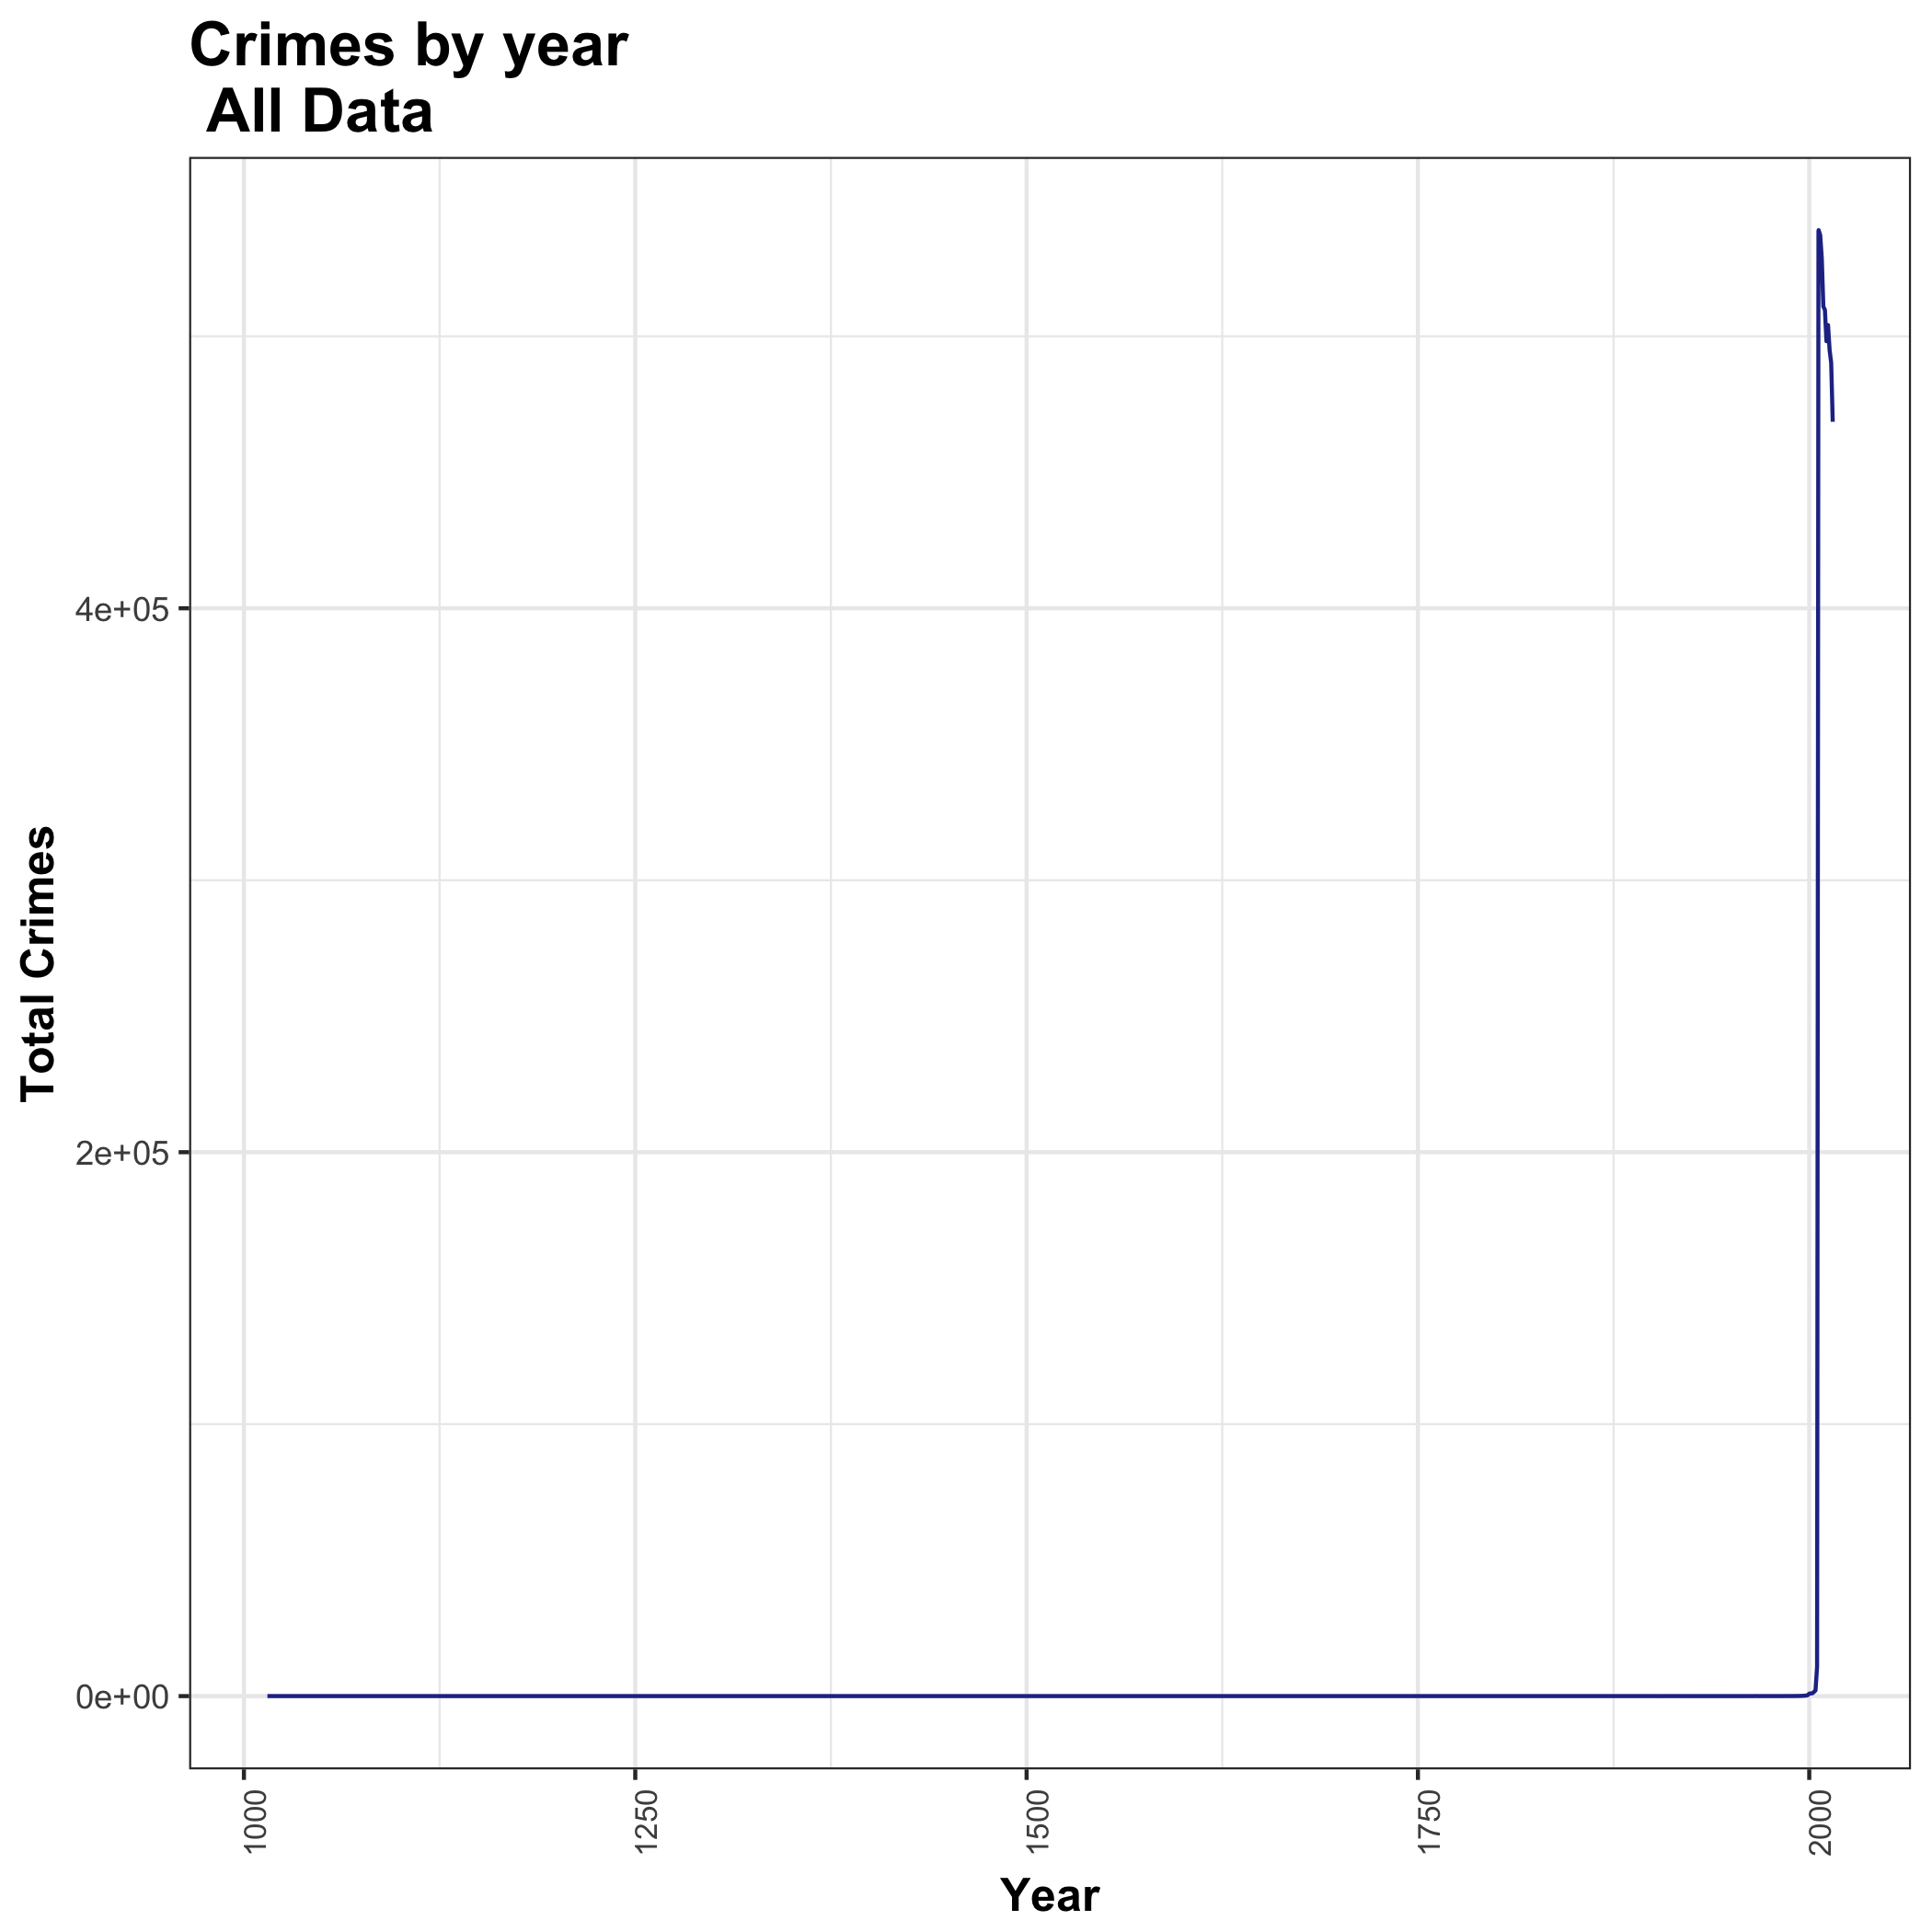
\includegraphics[scale=0.15]{1_YearlyAll.png}
\end{figure}

This plot shows one of the main issues of the data frame: There are 7 observations from the year 1015, a clear invalid value that should be taken out for analysis. But even after keeping all data from year 1990 ownwards, the problem doesn't seem to get better. There is clearly and under-reporting from 1990 until at least 2006, years where the data seems to be captured way after the crime happened. This is even more evident when a Log-scale is applied to Total Crimes, the y-axis.

\begin{figure}[H]
\centering
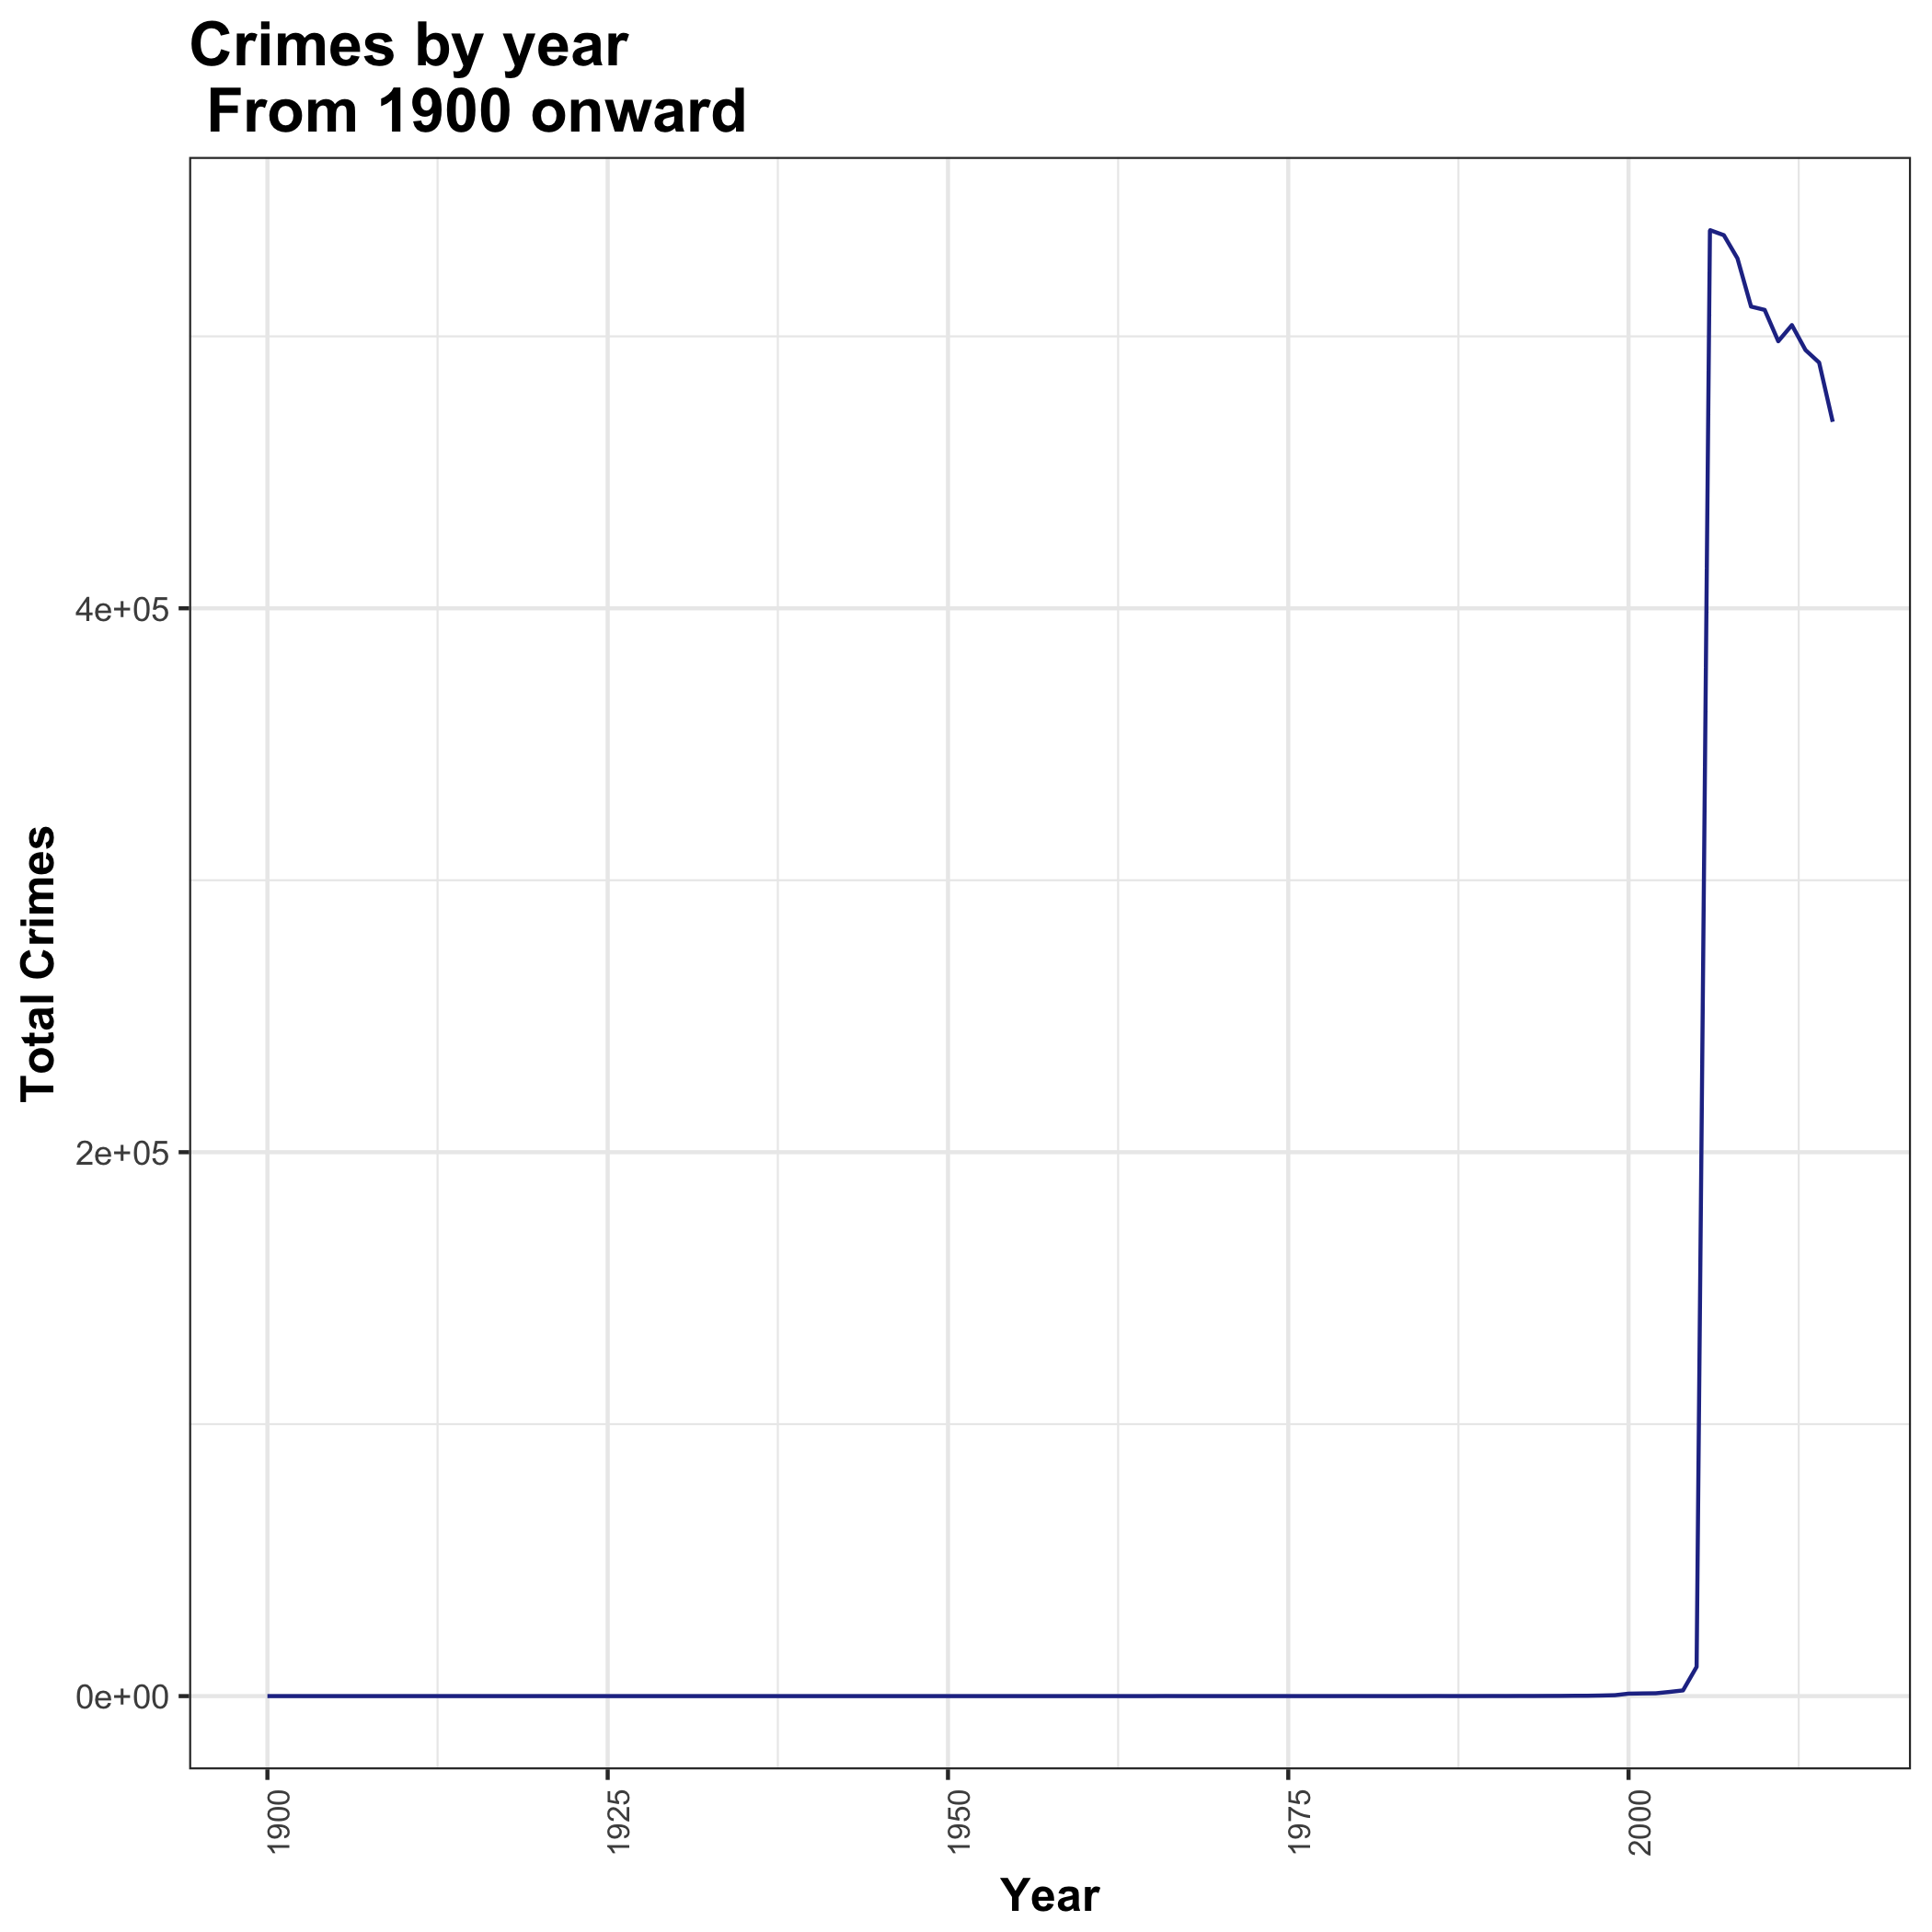
\includegraphics[scale=0.15]{2_YearlyFrom1900.png}
\end{figure}

\begin{figure}[H]
\centering
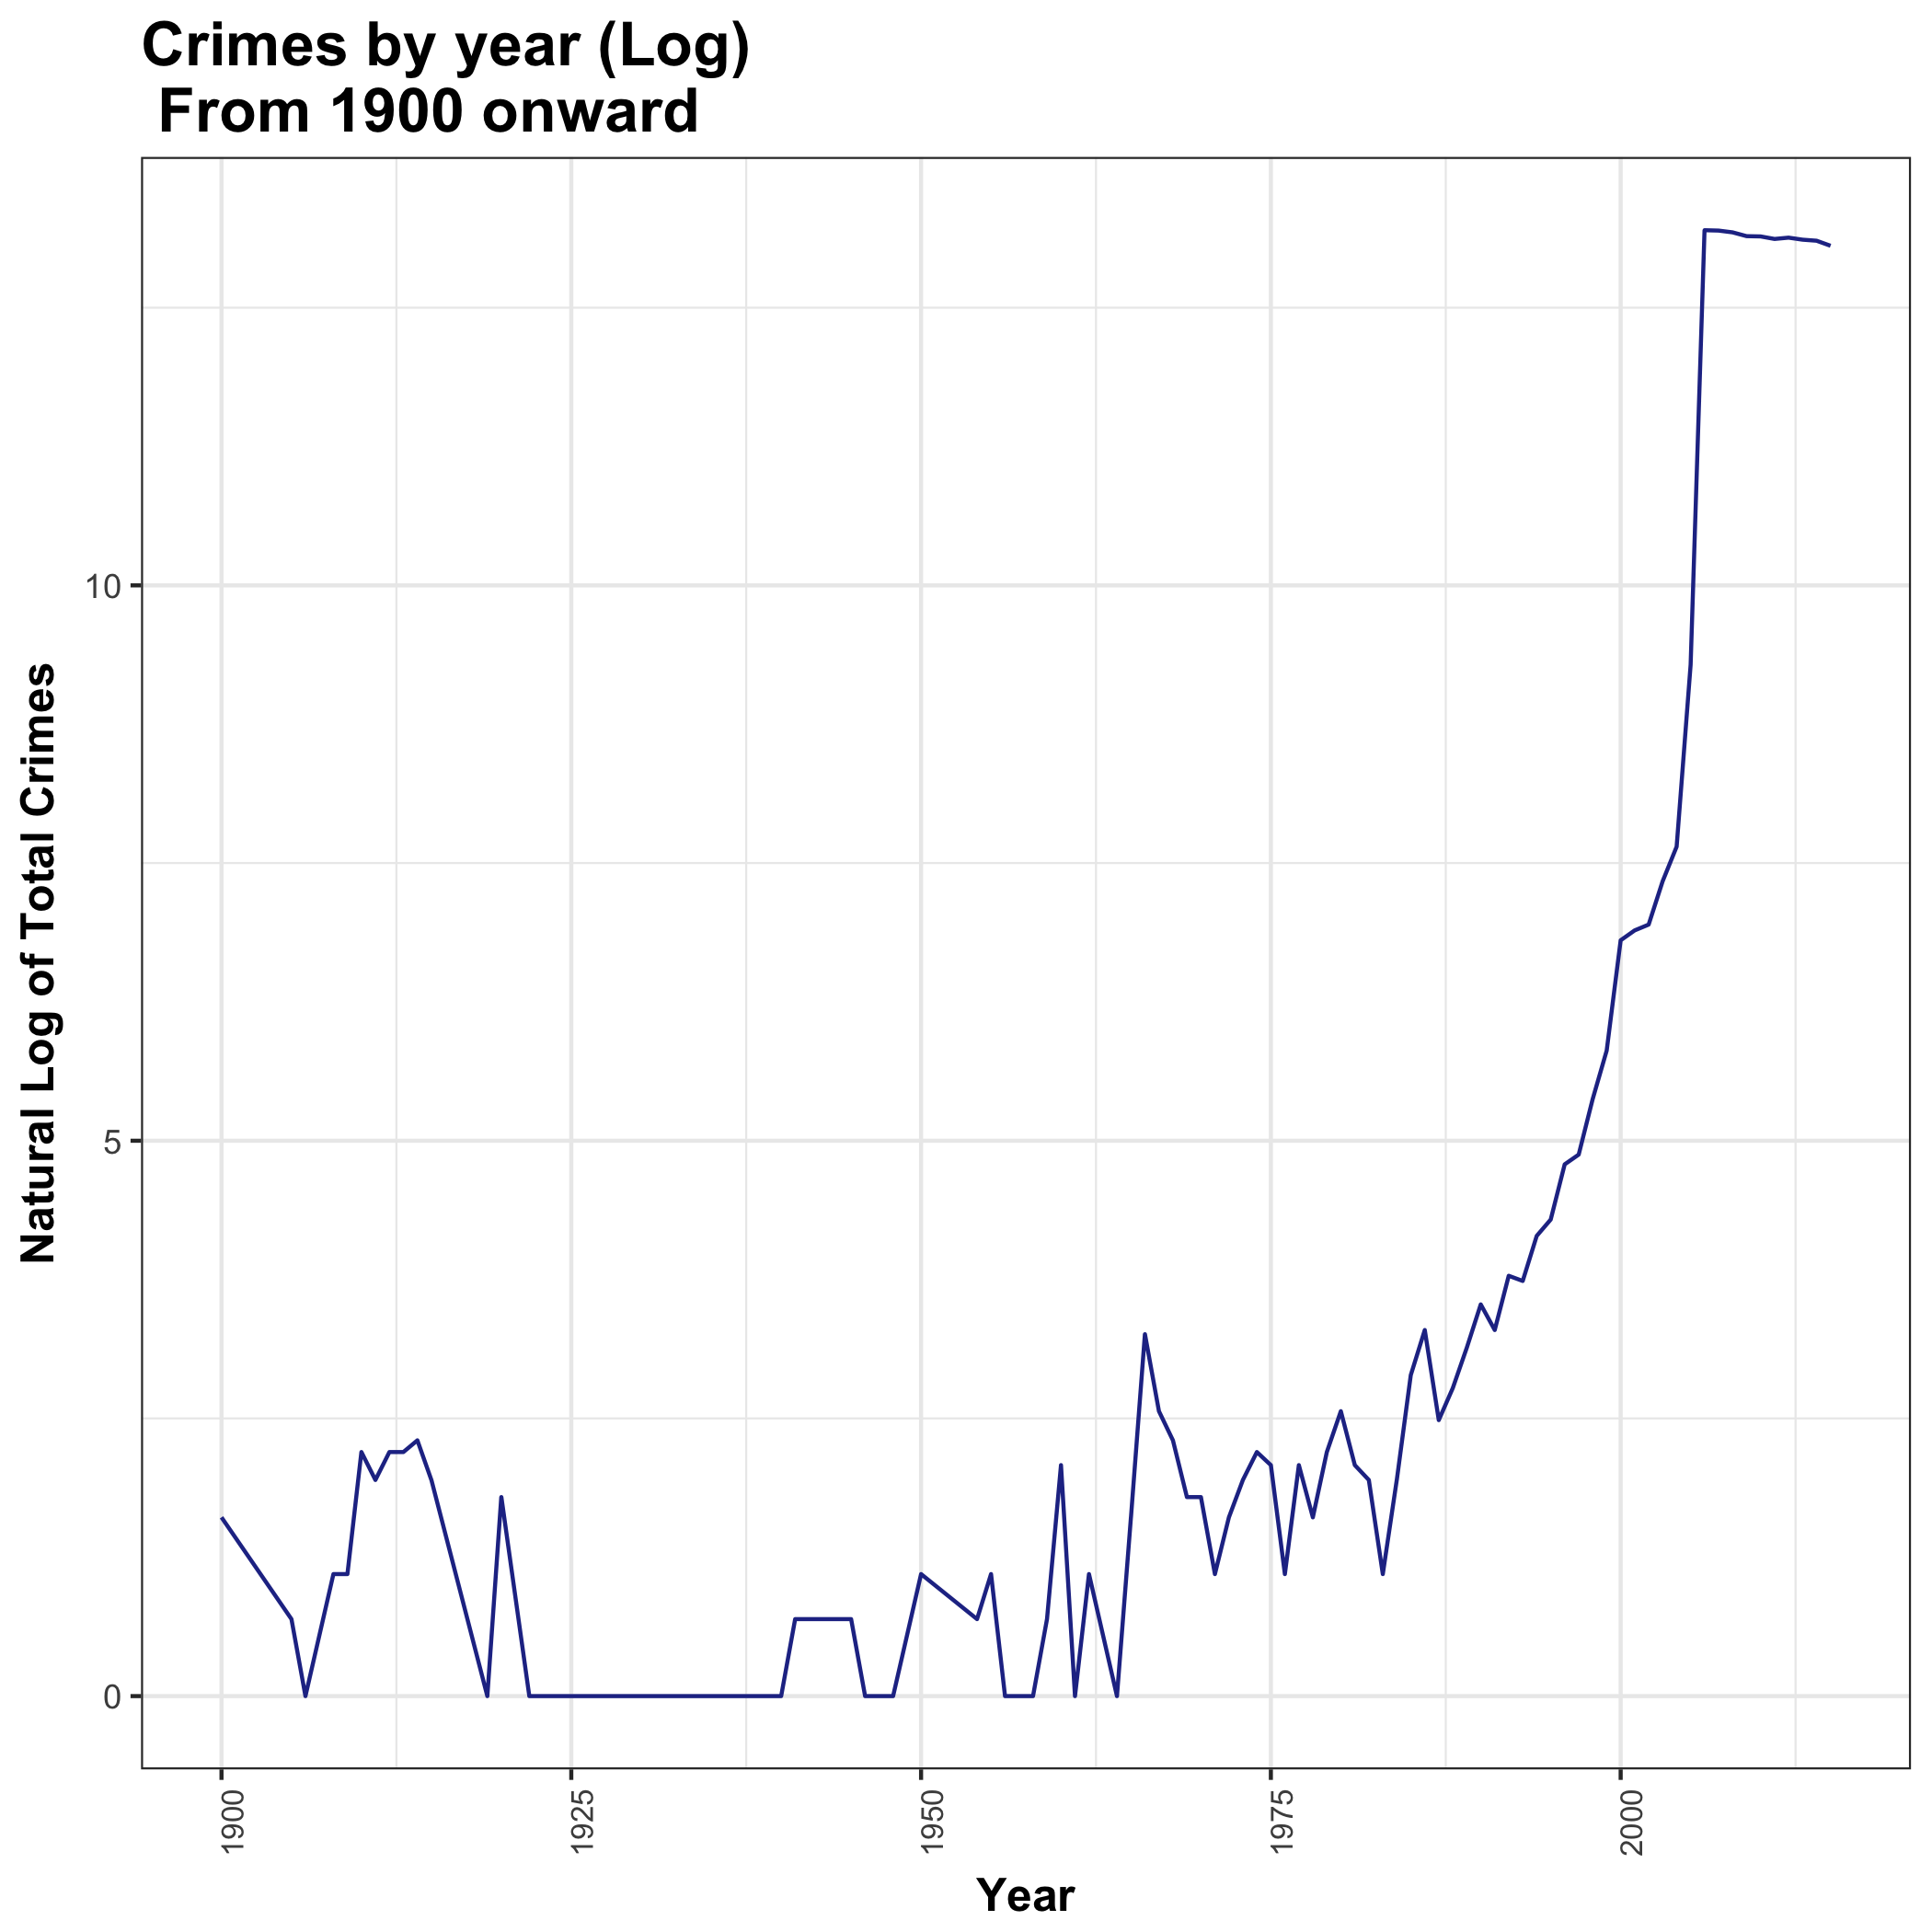
\includegraphics[scale=0.15]{3_LogYearlyFrom1900.png}
\end{figure}

After these, we decided that one issue that was worth inspecting is the difference between year of occurrence (captured in \texttt{CMPLNT\_FR\_DT}) and year of reporting (from the column \texttt{RPT\_DT}. The instability of this measure is staggering when we consider all years of occurrence after 1900.   

\begin{figure}[H]
\centering
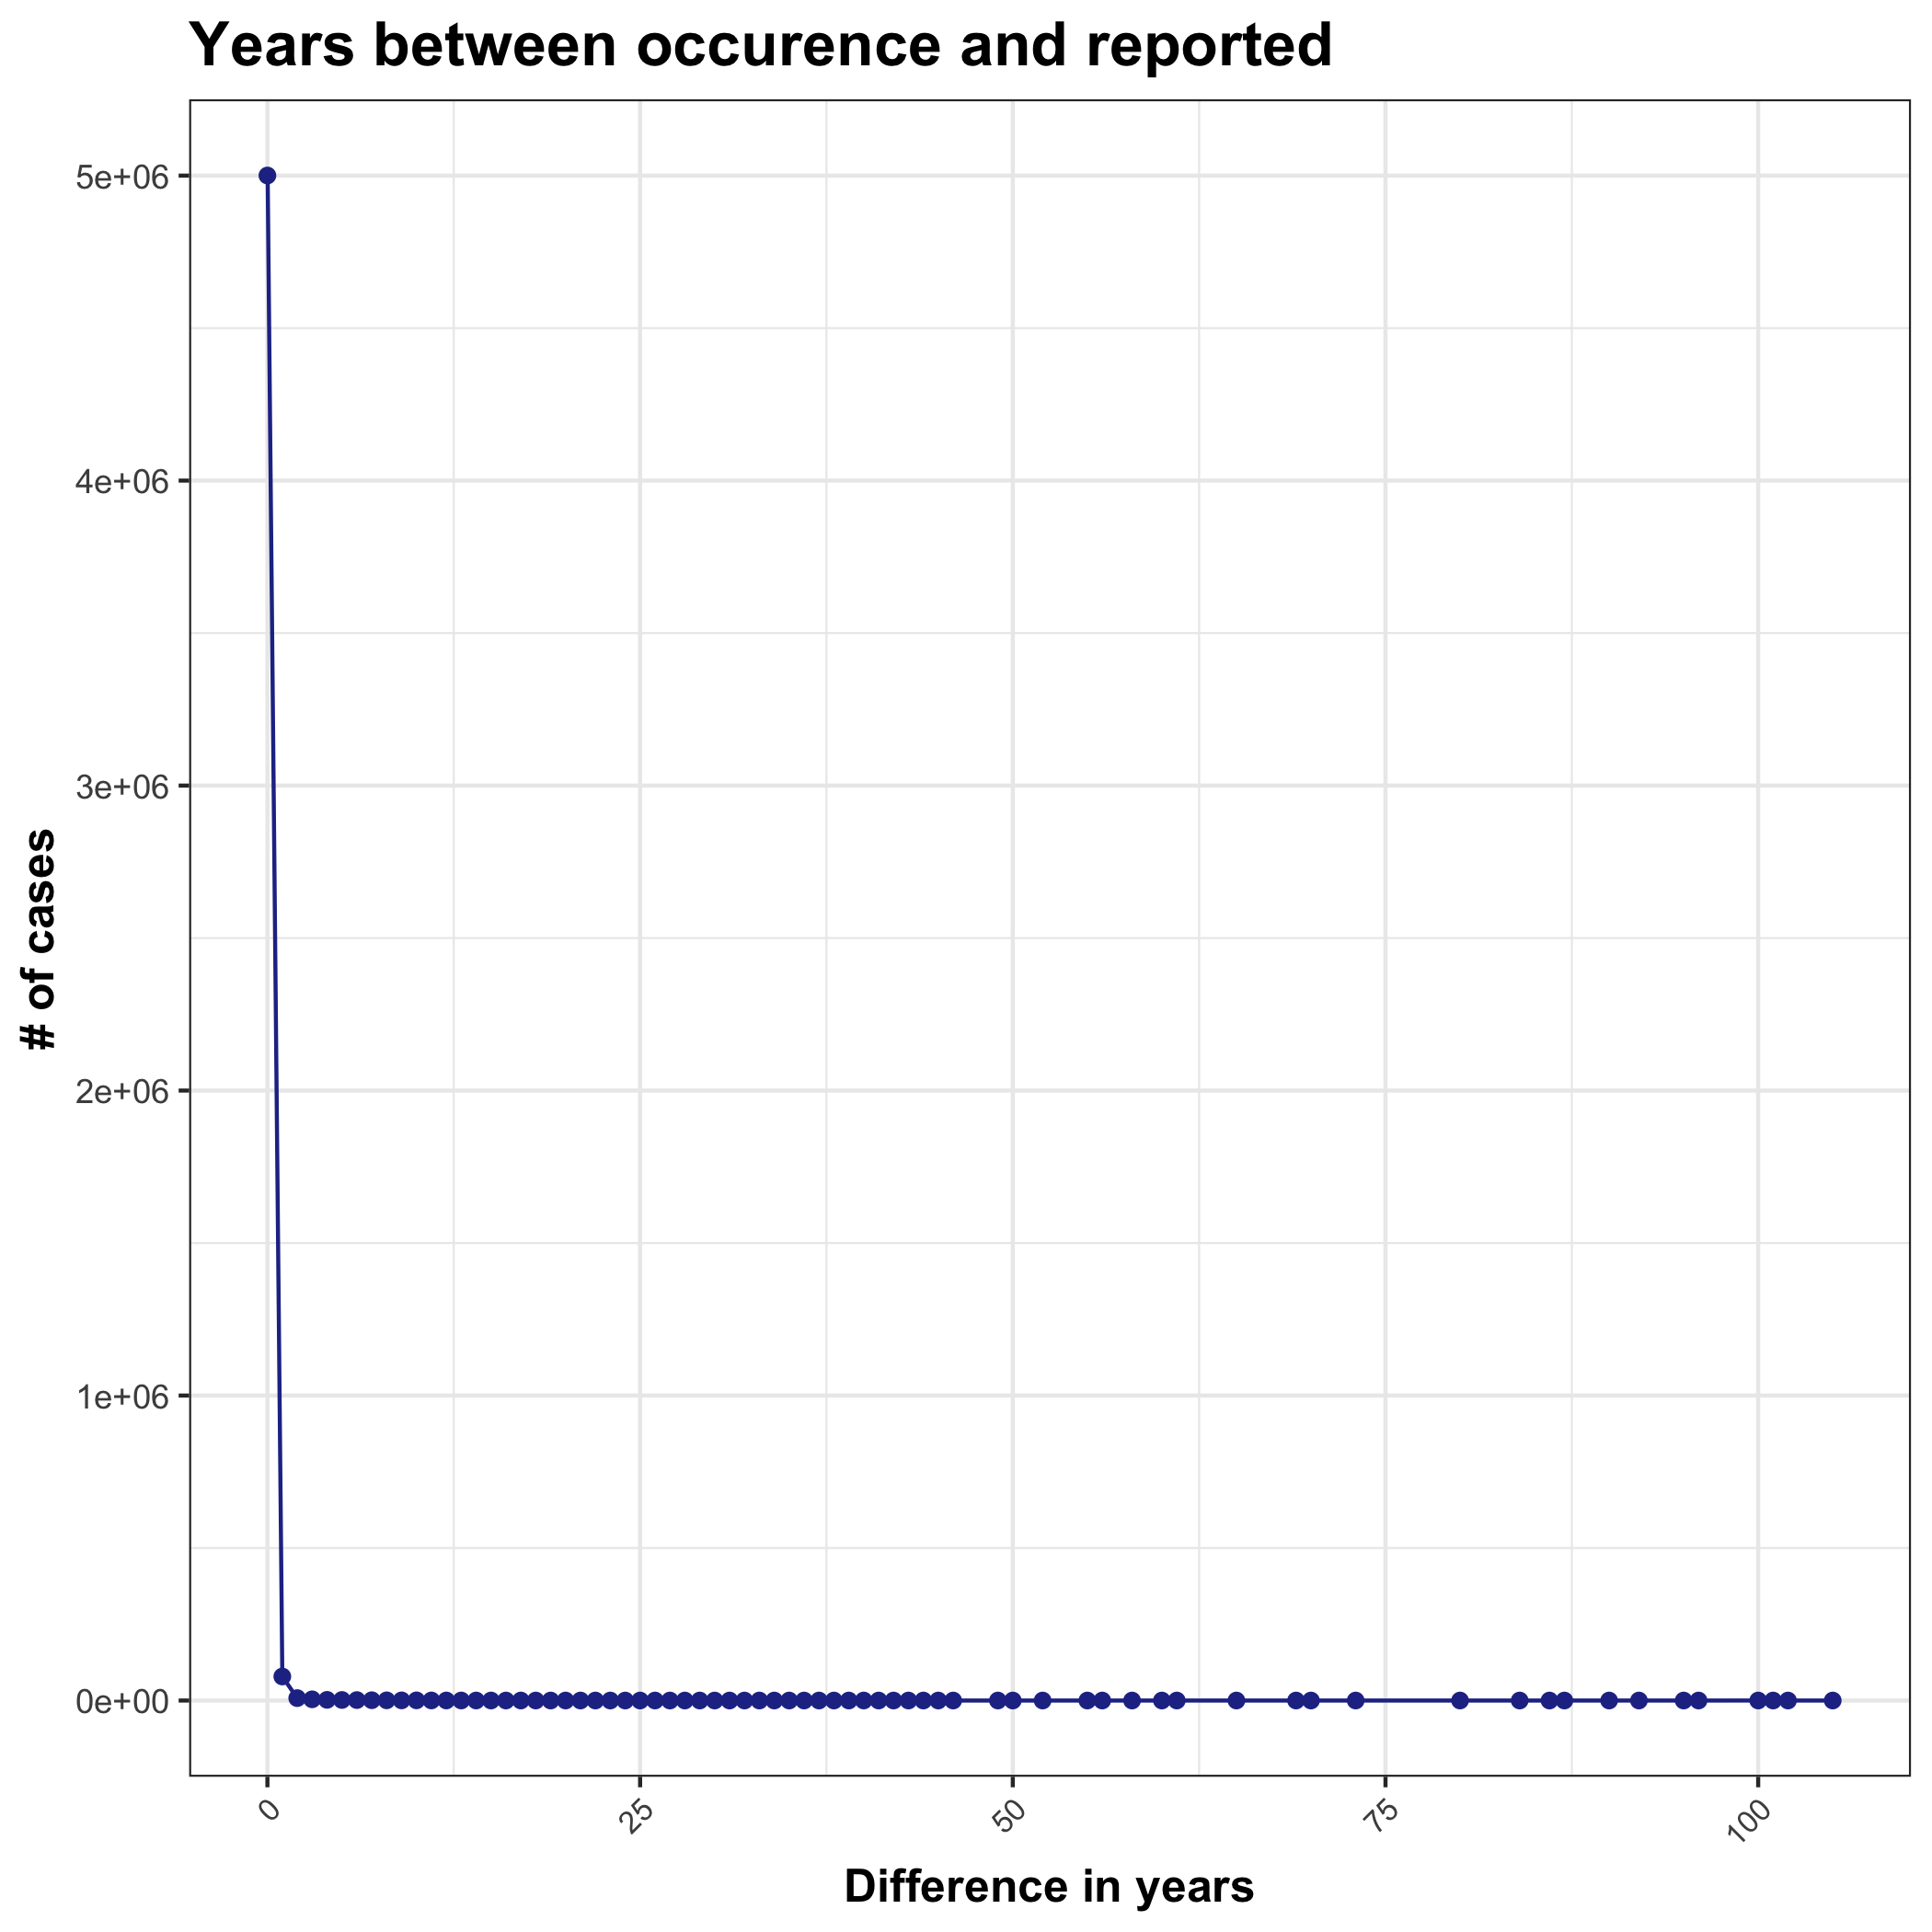
\includegraphics[scale=0.14]{8_DiffYears.png}
\end{figure}

\begin{figure}[H]
\centering
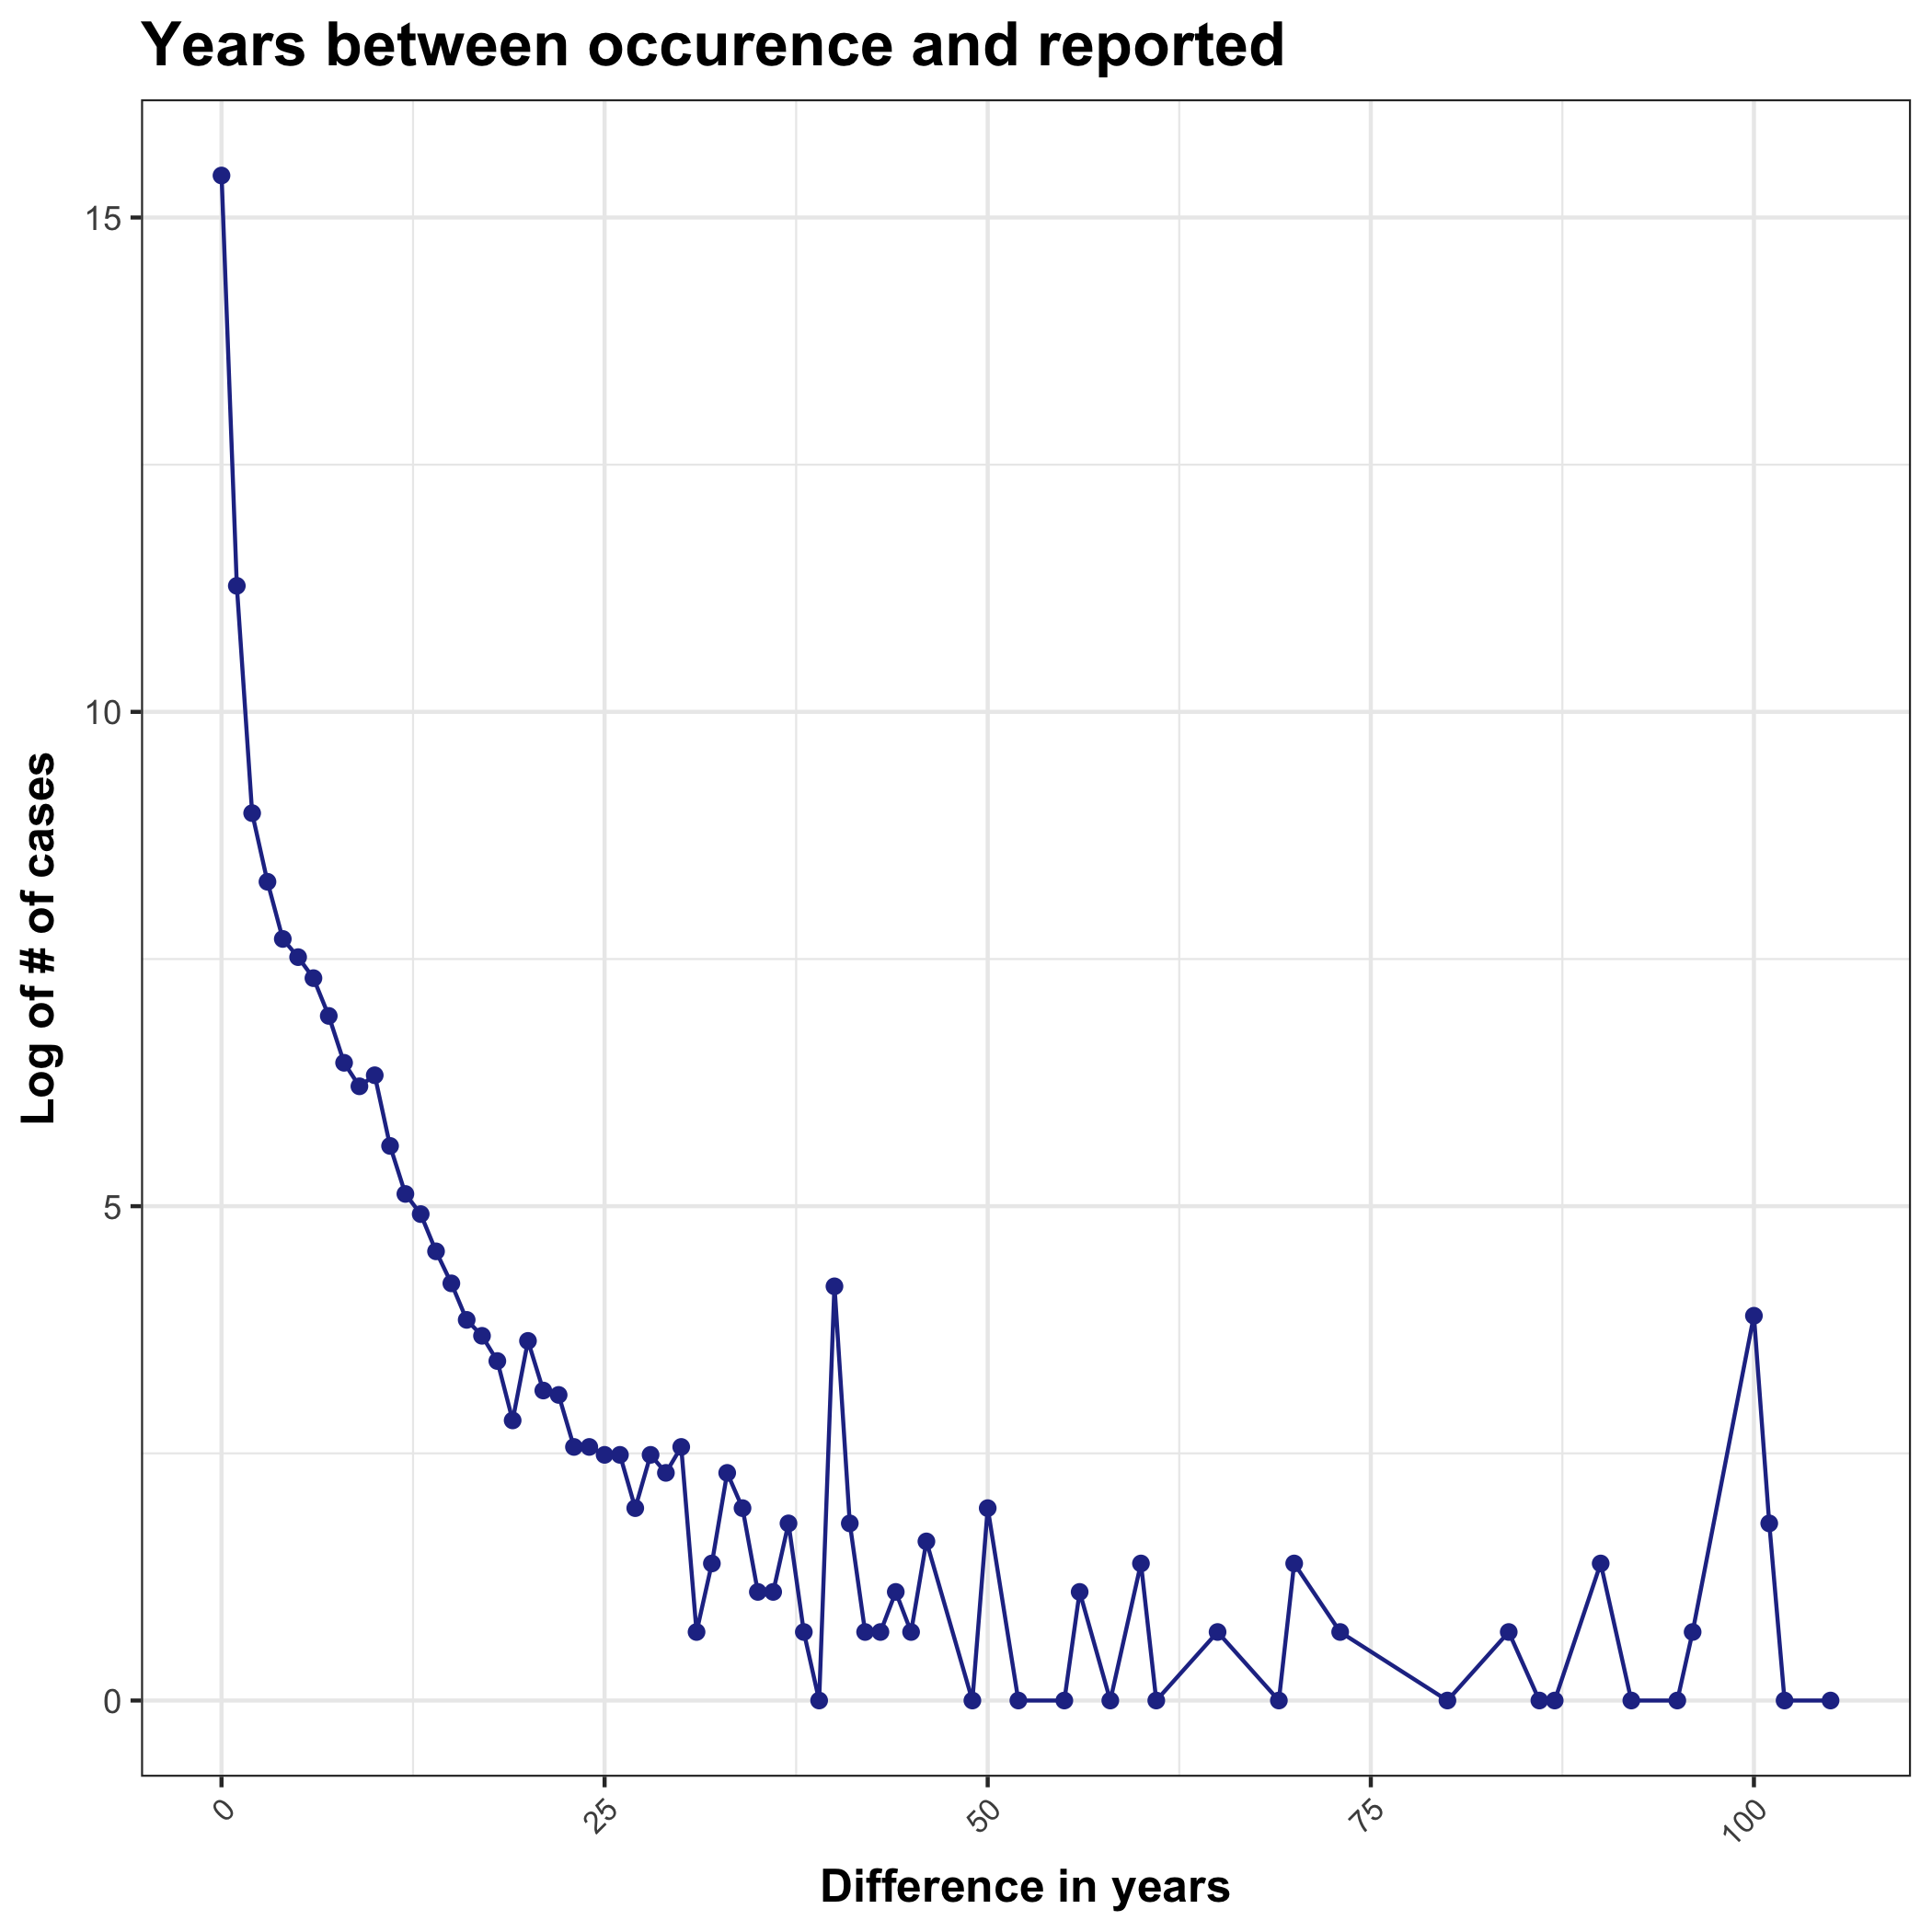
\includegraphics[scale=0.14]{9_LogDiffYears.png}
\end{figure}

Although most of the crimes are reported on the same year (98\% of all data) or the year after (1.5\%, probably due to crimes in December and reported on January next year), there are a large number of crimes with huge difference between the year it was reported and committed. For example, there are 49 crimes with a difference of 100 years between occurrence and reporting. By seeing the data, we can almost confirm, for example, that these cases have been miscoded for year of occurrence: 

\begin{center}
\textbf{Cases with 100 years of difference between occurrence and reporting} \\
\begin{tabular}{ |c|c|c| } 
\hline
\textbf{Year occurrence} & \textbf{Year reported}  & \textbf{Number of cases} \\
\hline
   1909 & 2009 & 1 \\ 
   1912 & 2012 & 9 \\ 
   1910 & 2010 & 7 \\  
   1913 & 2013 & 7 \\  
   1914 & 2014 & 9 \\ 
   1906 & 2006 & 1 \\ 
   1915 & 2015 & 7 \\ 
   1911 & 2011 & 6\\ 
   1908 & 2008 & 3 \\ 
\hline
\end{tabular}
\end{center}

The question then is: Should we recod this cases? Add 100 years to them? Or simply discard them? To answer this question, let us first do the same plots as above, but only with the years 2006 ownwards: 

\begin{figure}[H]
\centering
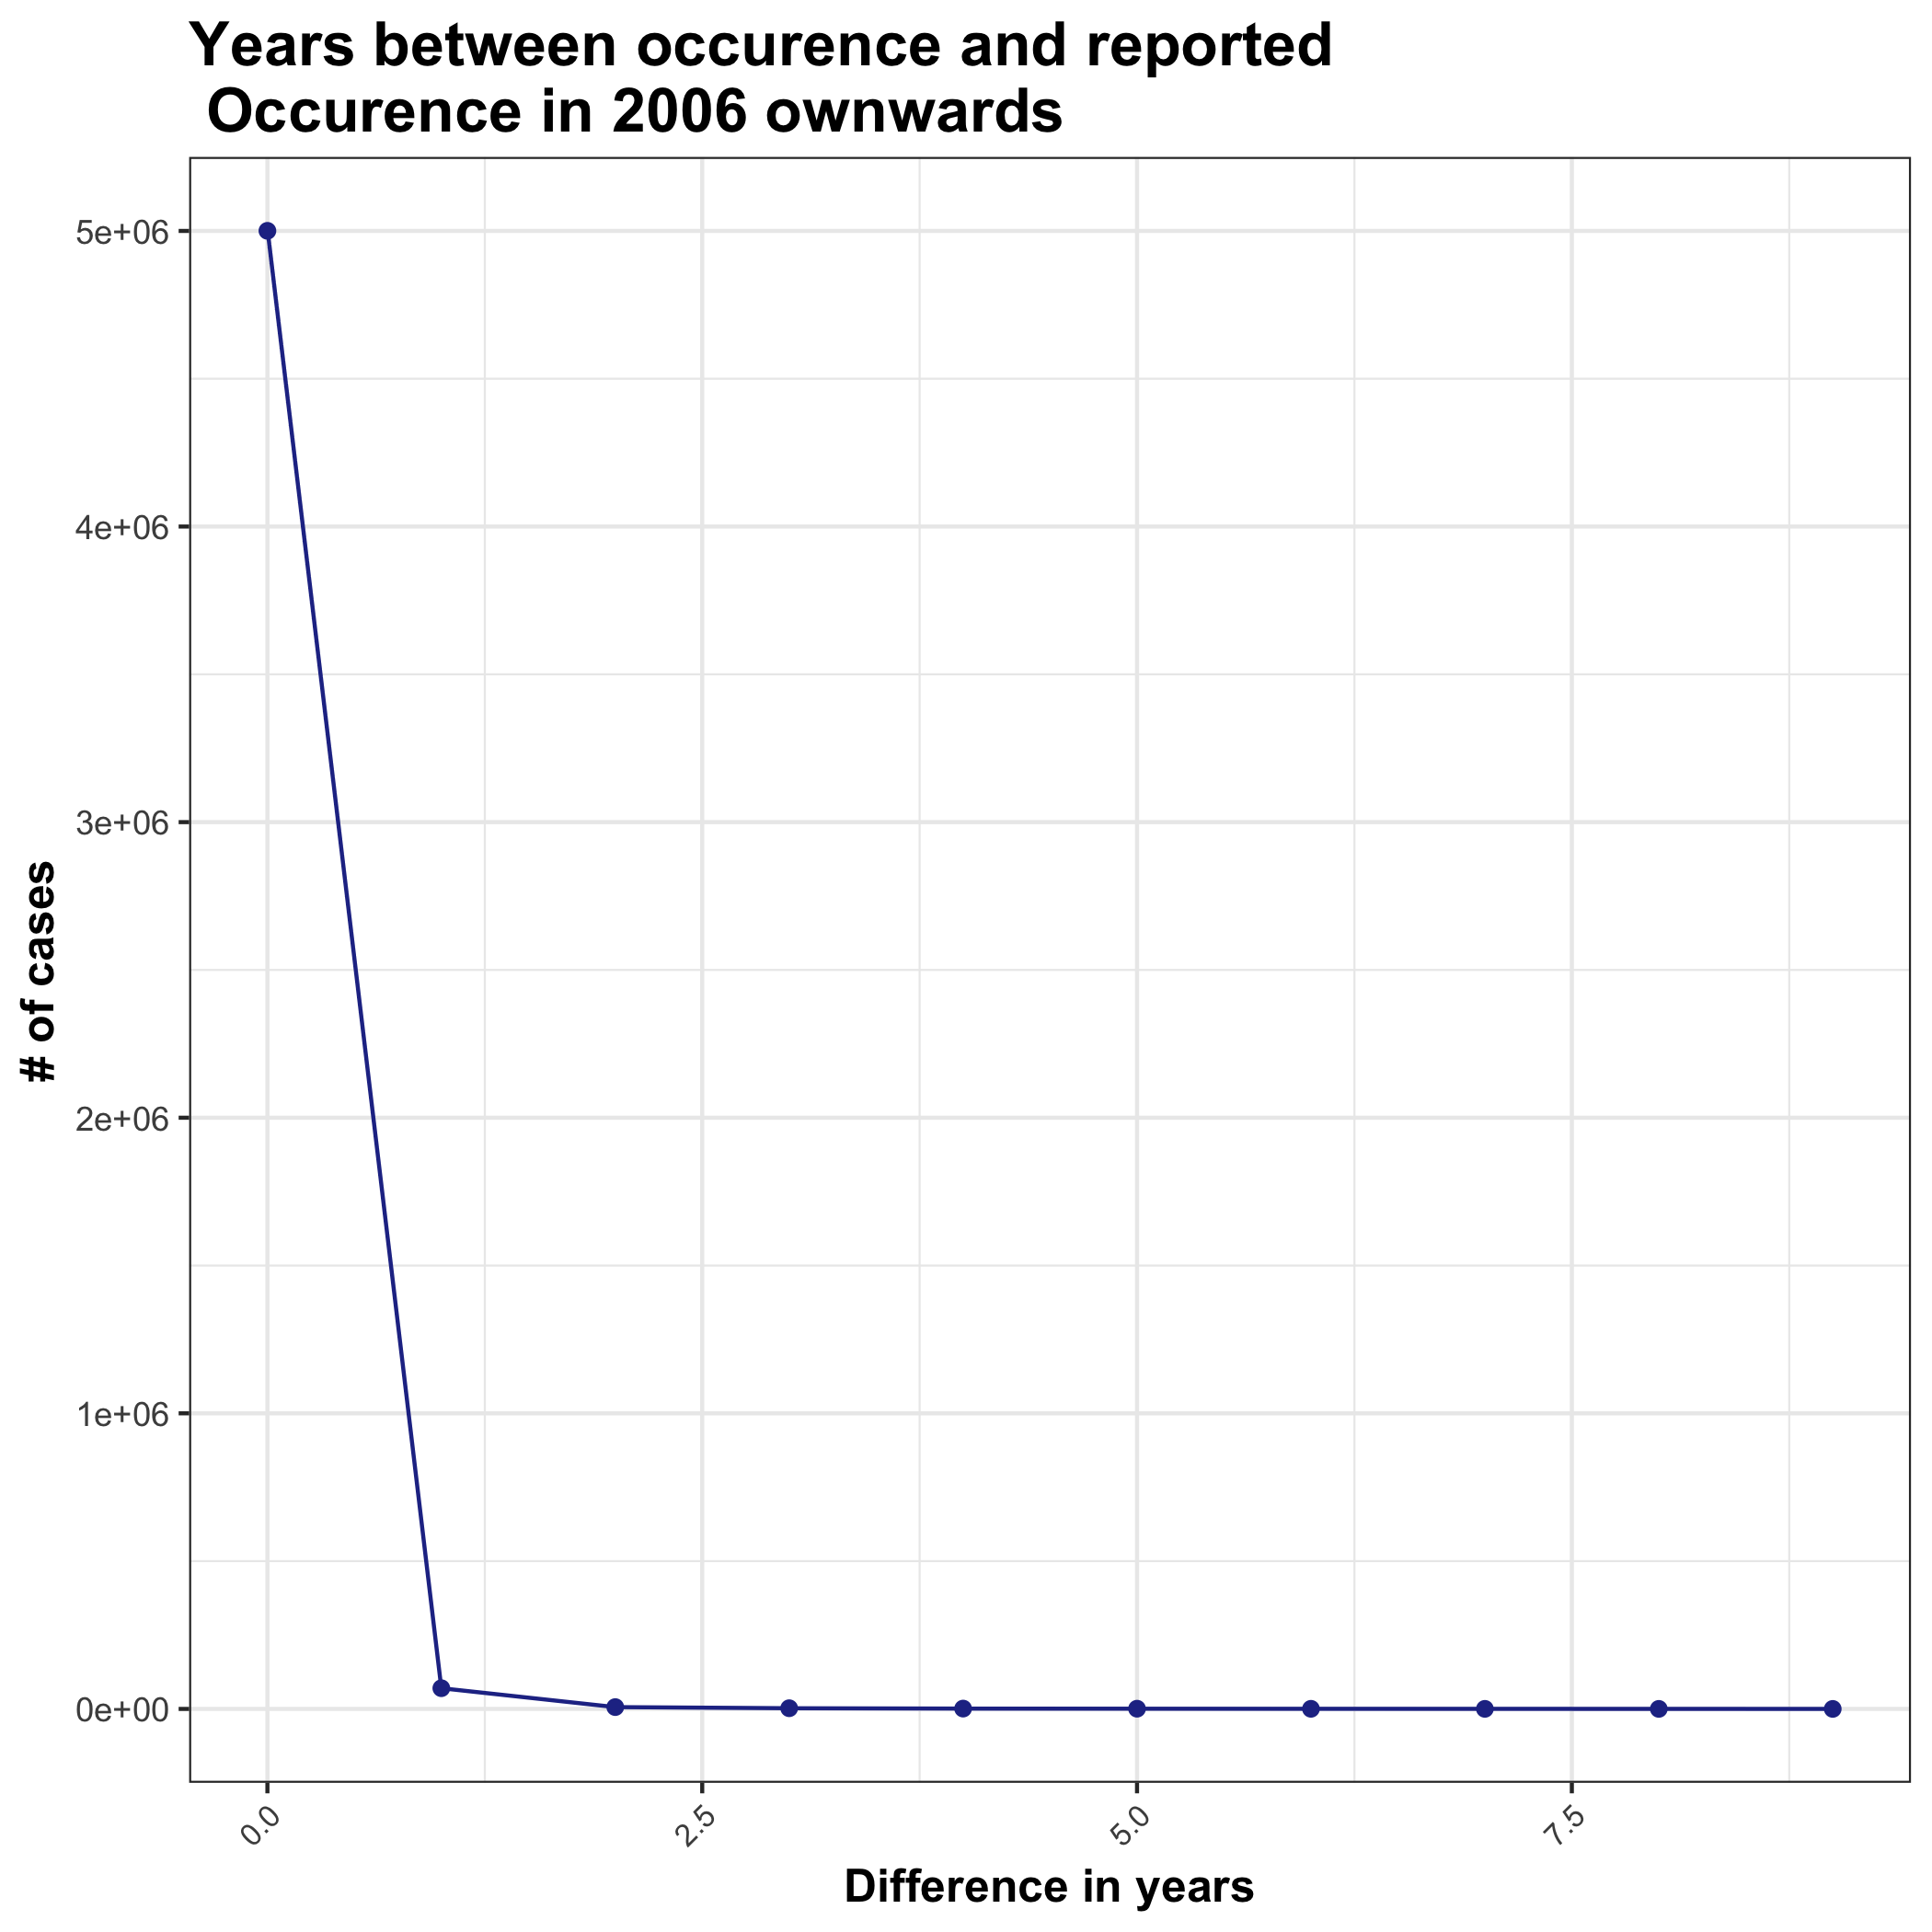
\includegraphics[scale=0.14]{10_DiffYears_2006.png}
\end{figure}

\begin{figure}[H]
\centering
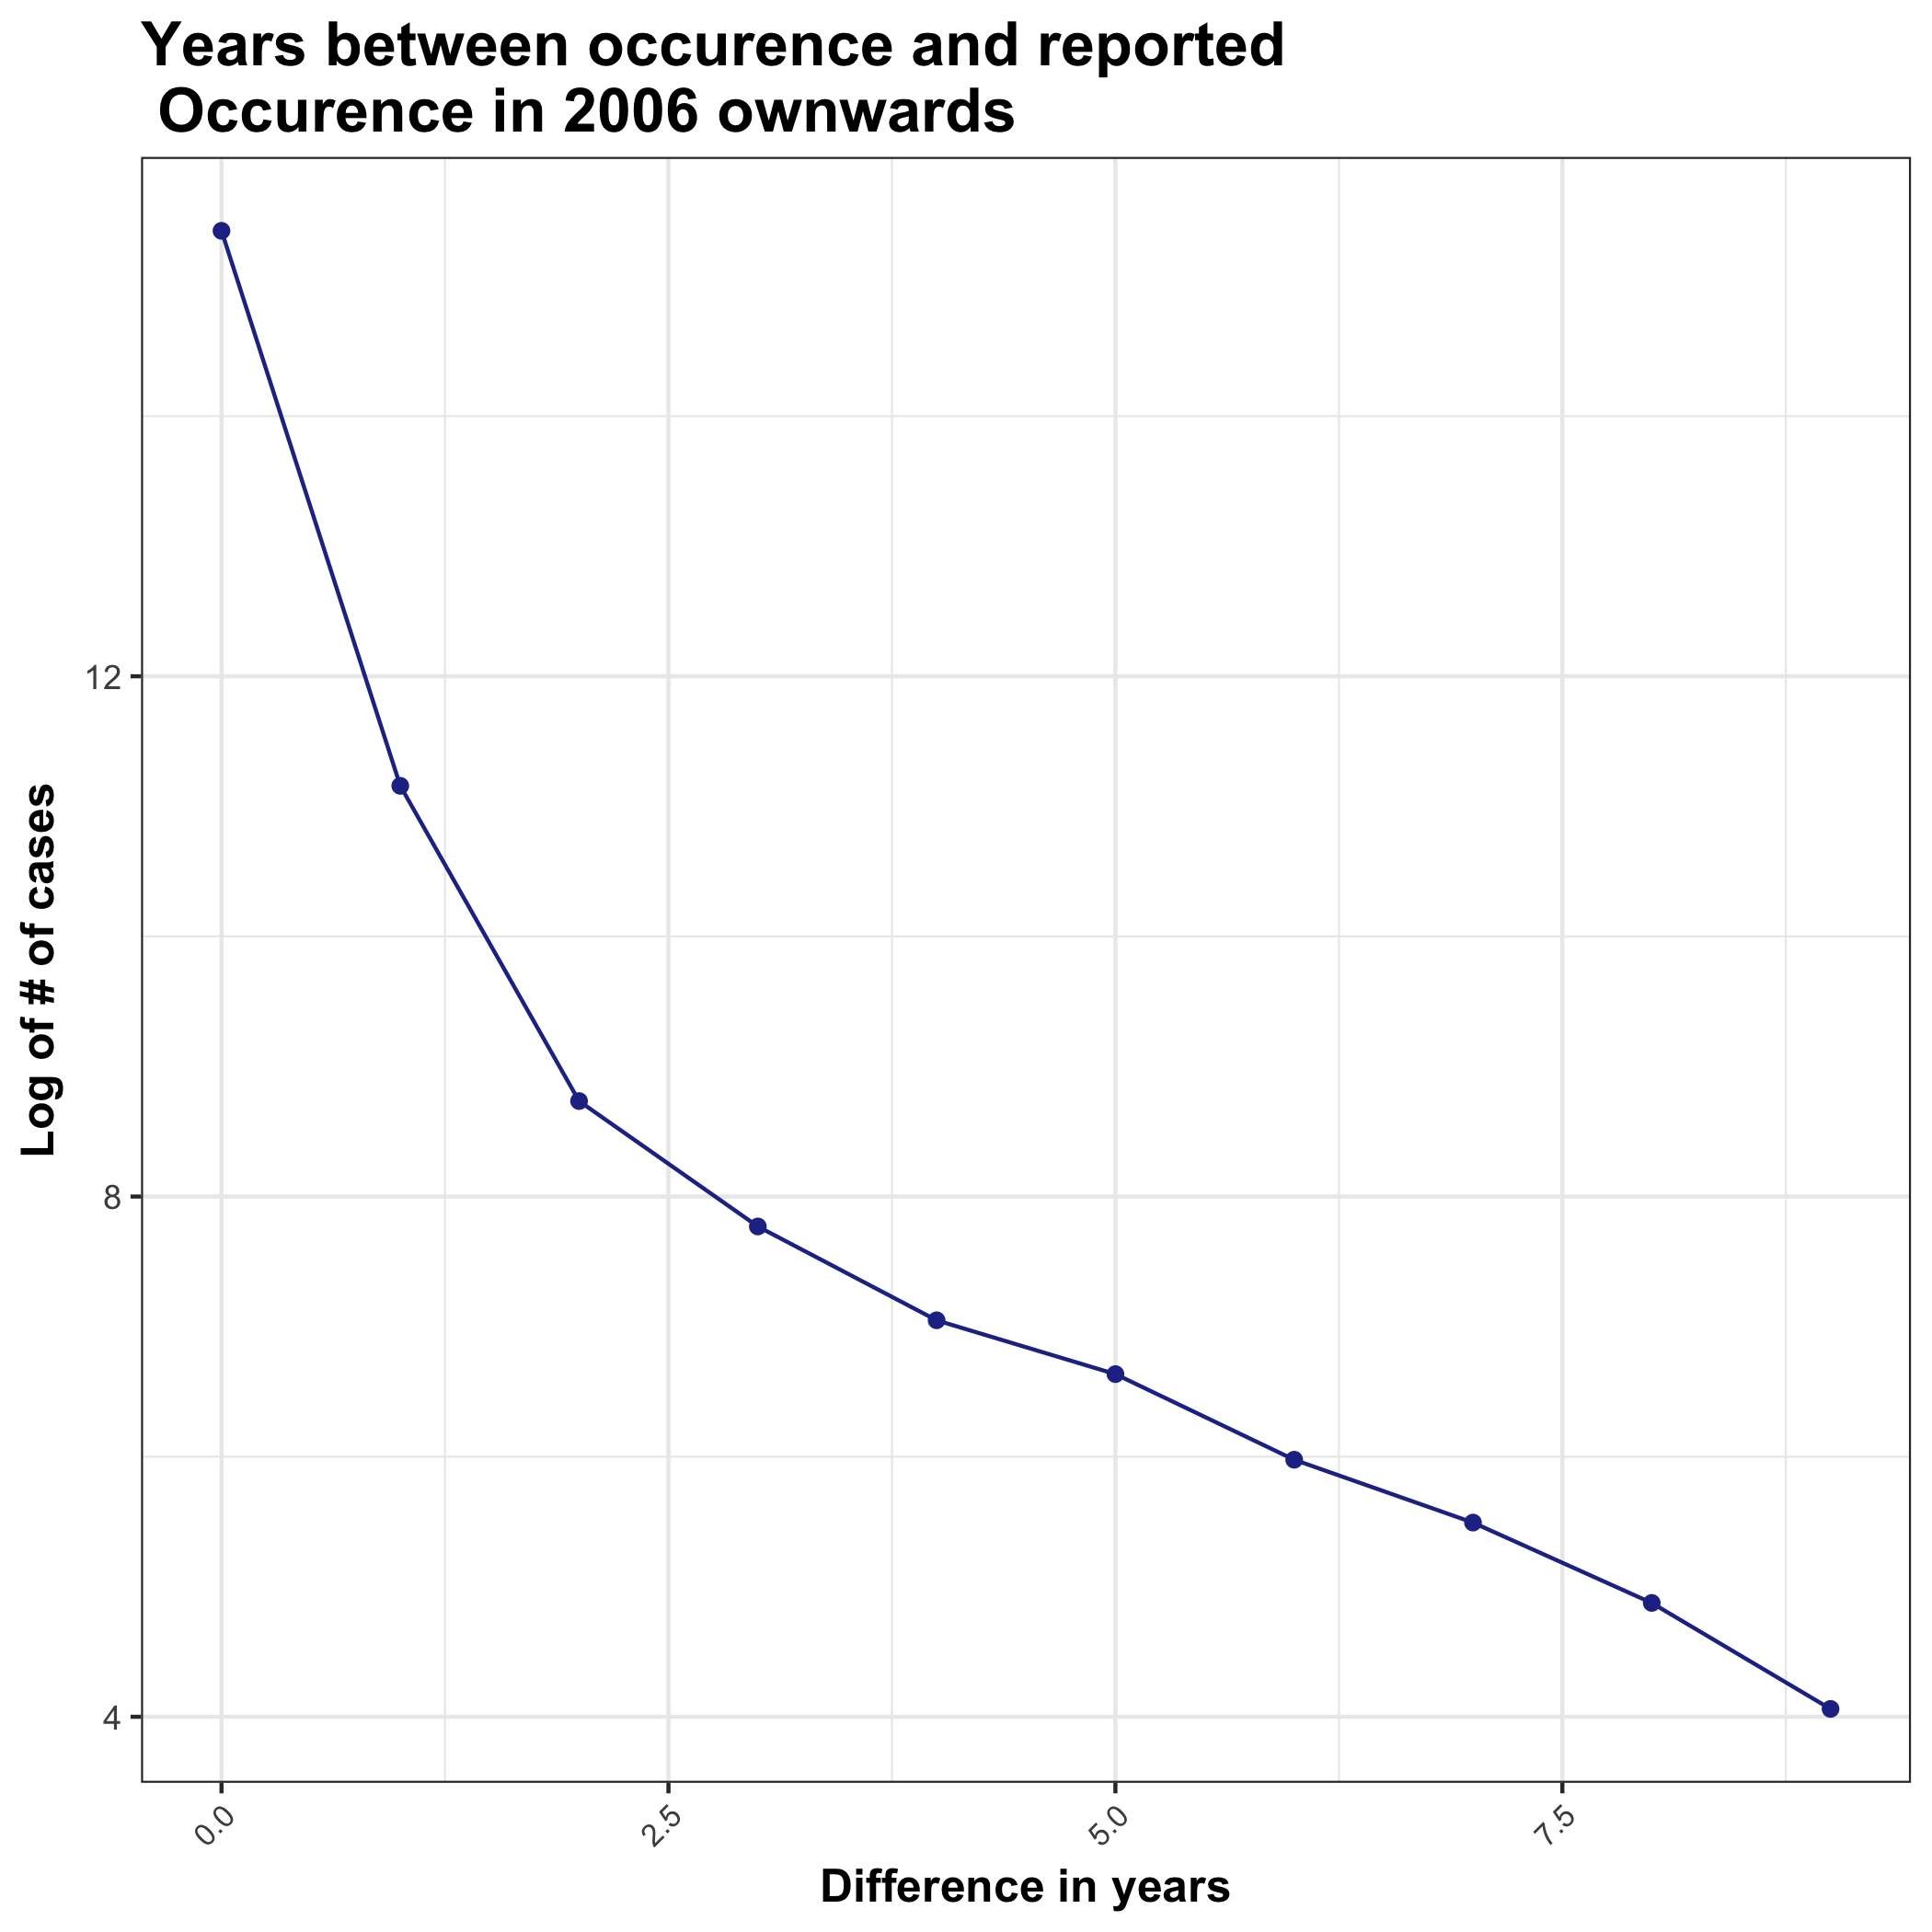
\includegraphics[scale=0.14]{11_LogDiffYears_2006.png}
\end{figure}

In this case, we can see what it looks like a natural and more steady line of descent between year of reporting and year of occurence. This, it is our believe, are valid cases: Some crimes just take a long time to be reported, maybe because of the victim is simply traumatized, or maybe because there are crimes that can las for years. In any case, it looks to us that the best strategy for the analytic section is going to be to keep only the cases that have a year of occurrence from 2006 onwards, and in fact discarding the cases that have been miscoded for year. 

That being said, we continued with a similar analysis with the time of occurrence. At first, we decided to plot all the crimes by hour, to see if there were any differences by time of the day. As seen below, it's clear that most crimes are registered by the exact hour, but few have information about the exact minute when it was registered. 

\begin{figure}[H]
\centering
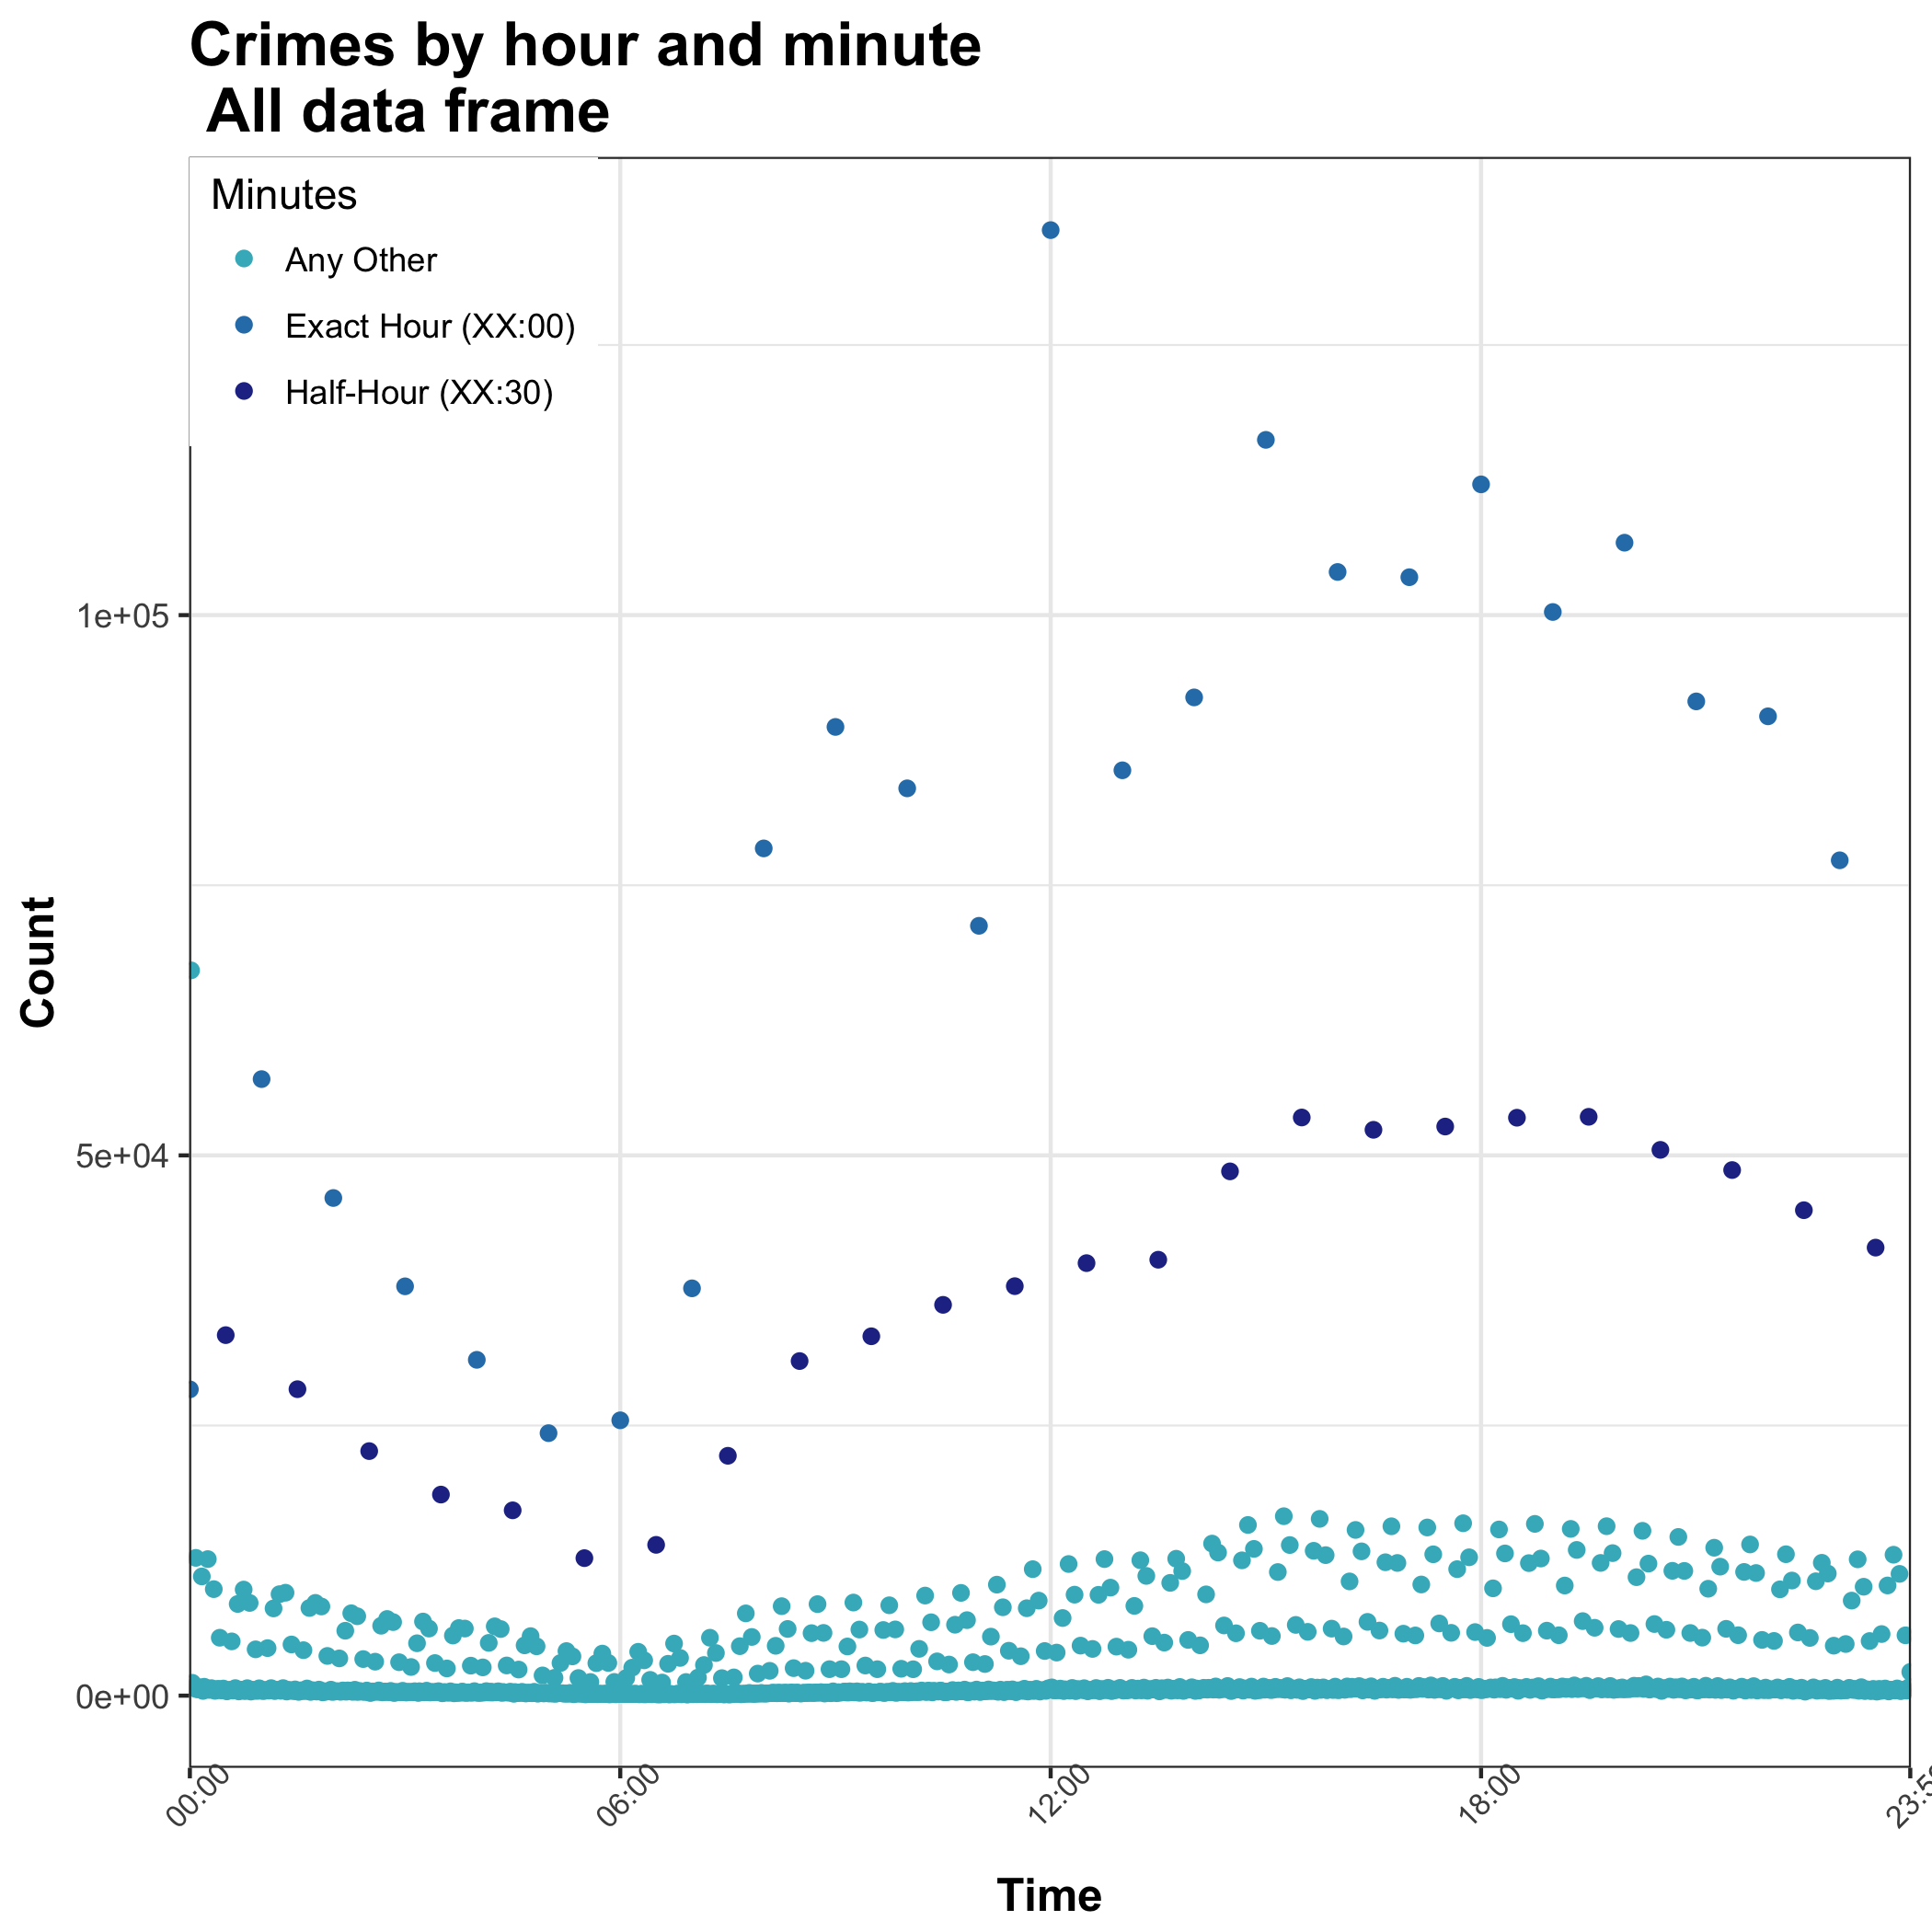
\includegraphics[scale=0.15]{4_HourMinute.png}
\end{figure}

To fix this and observe tendencies by time of the day, we decided to round the minutes to the hour (i.e., if a crime was registered at 6:01 or at 6:59, we consider it to be at 6:00). This lets us observe the tendency of crimes. Clearly, most of the crimes are committed between 3:00 pm and 8:00 pm. The following graph also shows us an issue: There is a slight spike when it comes to 12:00. Probably, many crimes when the time is not registered are encoded automatically to noon. 

\begin{figure}[H]
\centering
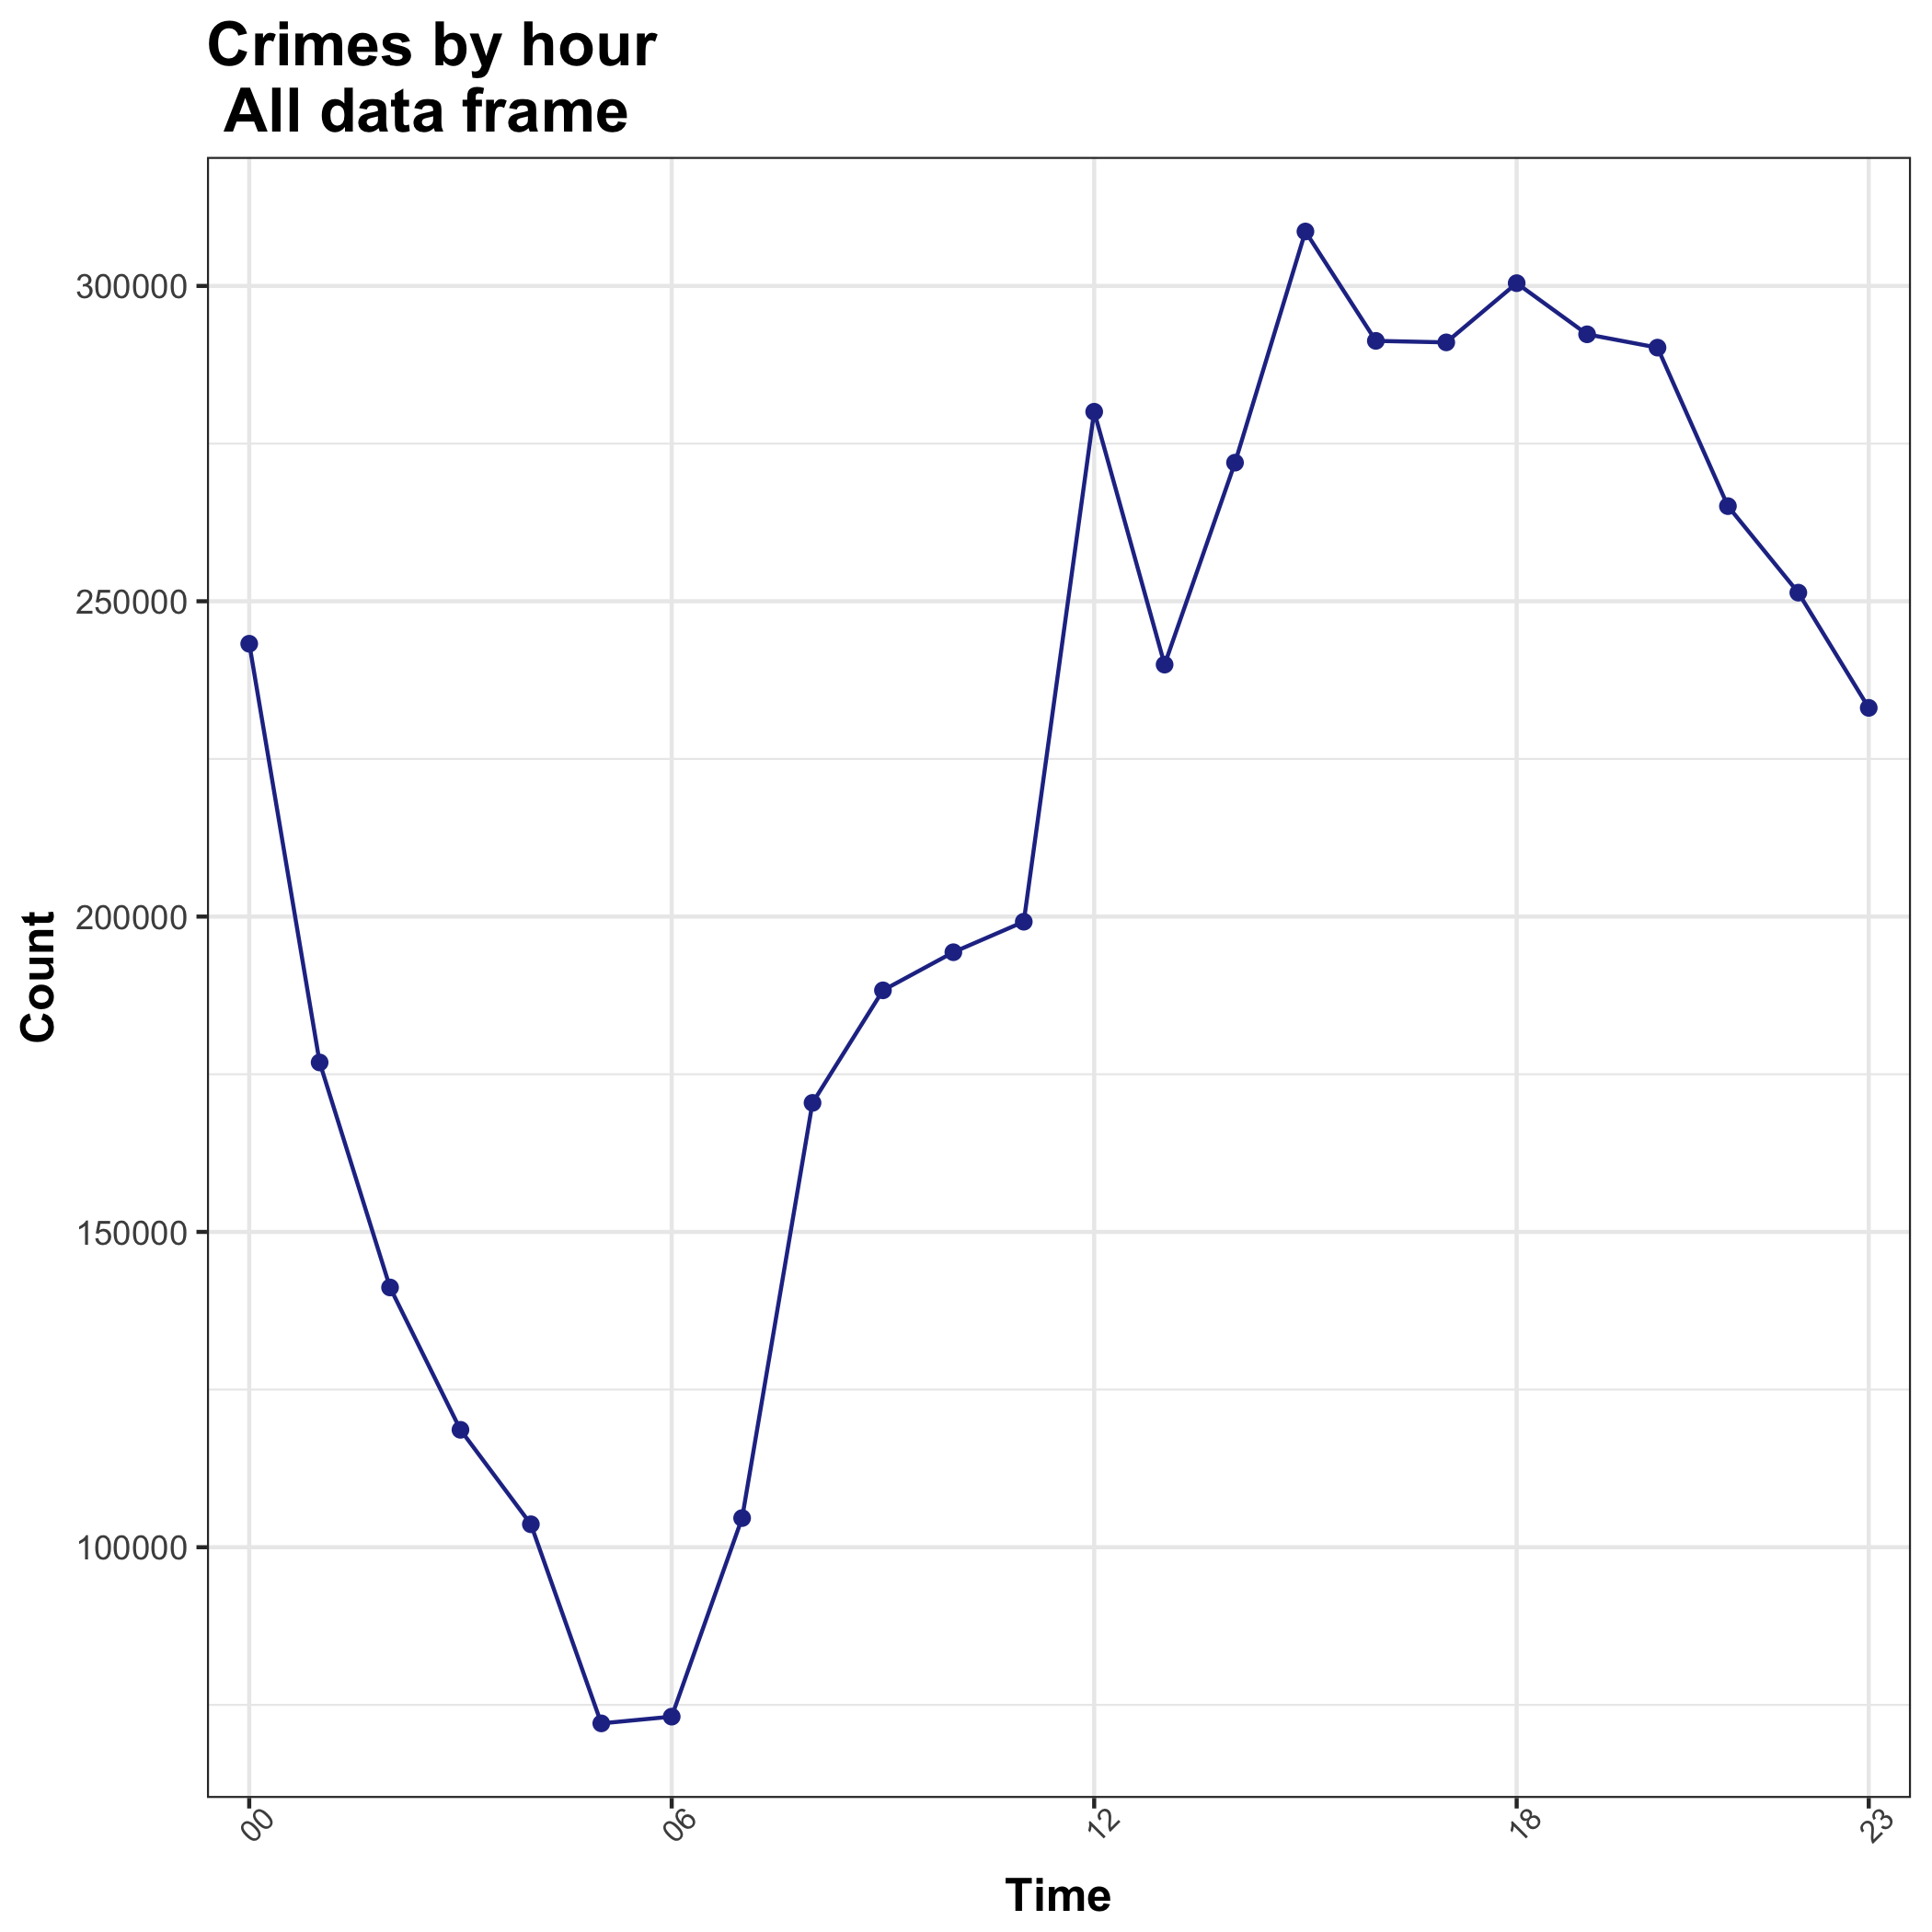
\includegraphics[scale=0.15]{5_Hour.png}
\end{figure}

Finally, we did a  a quick analysis by the type of crime, encoded in the column \texttt{OFNS\_DESC}. Before begin describing the main findings, it's worth noticing that the variables\texttt{KY\_CD} and \texttt{OFNS\_DESC} do not match one to one. For example, "abortion" has more than one code assigned to it. This, as it was stated above, could easily by analyzed if an external codebook for Crime ID was published. 

In any case, we took all the crimes from 2006 to make an analysis of the most common type of crimes in New York City. From this year on, there are 18,775 with no type. Out of 5081794 (this is, 0.36\% of the data). Some categories, like the crime for "Fortune Telling" has only one observation, a crime apparently committed in 2015. The 6 main categories add a total of 3,222,141 crimes, representing  63.64\% of the data. Murder ("MURDER \& NON-NEGL. MANSLAUGHTER"), on the other hand, has only 4444 cases from 2006, barely 0.008\% of the crimes committed in NYC. Rape, another crime that might be of particular interest, has 12,986 cases on the data frame, and Sex Crimes (we assume, other that rape), 53,213 cases. 

We also decided to perform a quick analysis of the 6 main crimes in NYC over 2006 - 2015. From this, only "Dangerous Drugs" seem to have a negative trend over time: From 2006 to 2015, the crimes for this category went from 36126 to 23645, a reduction of 34.5\%. Other crimes, as HARRASSMENT, seem to have declined until 2013, to see later a spike towards 2014 and 2015. 


\begin{figure}[H]
\centering
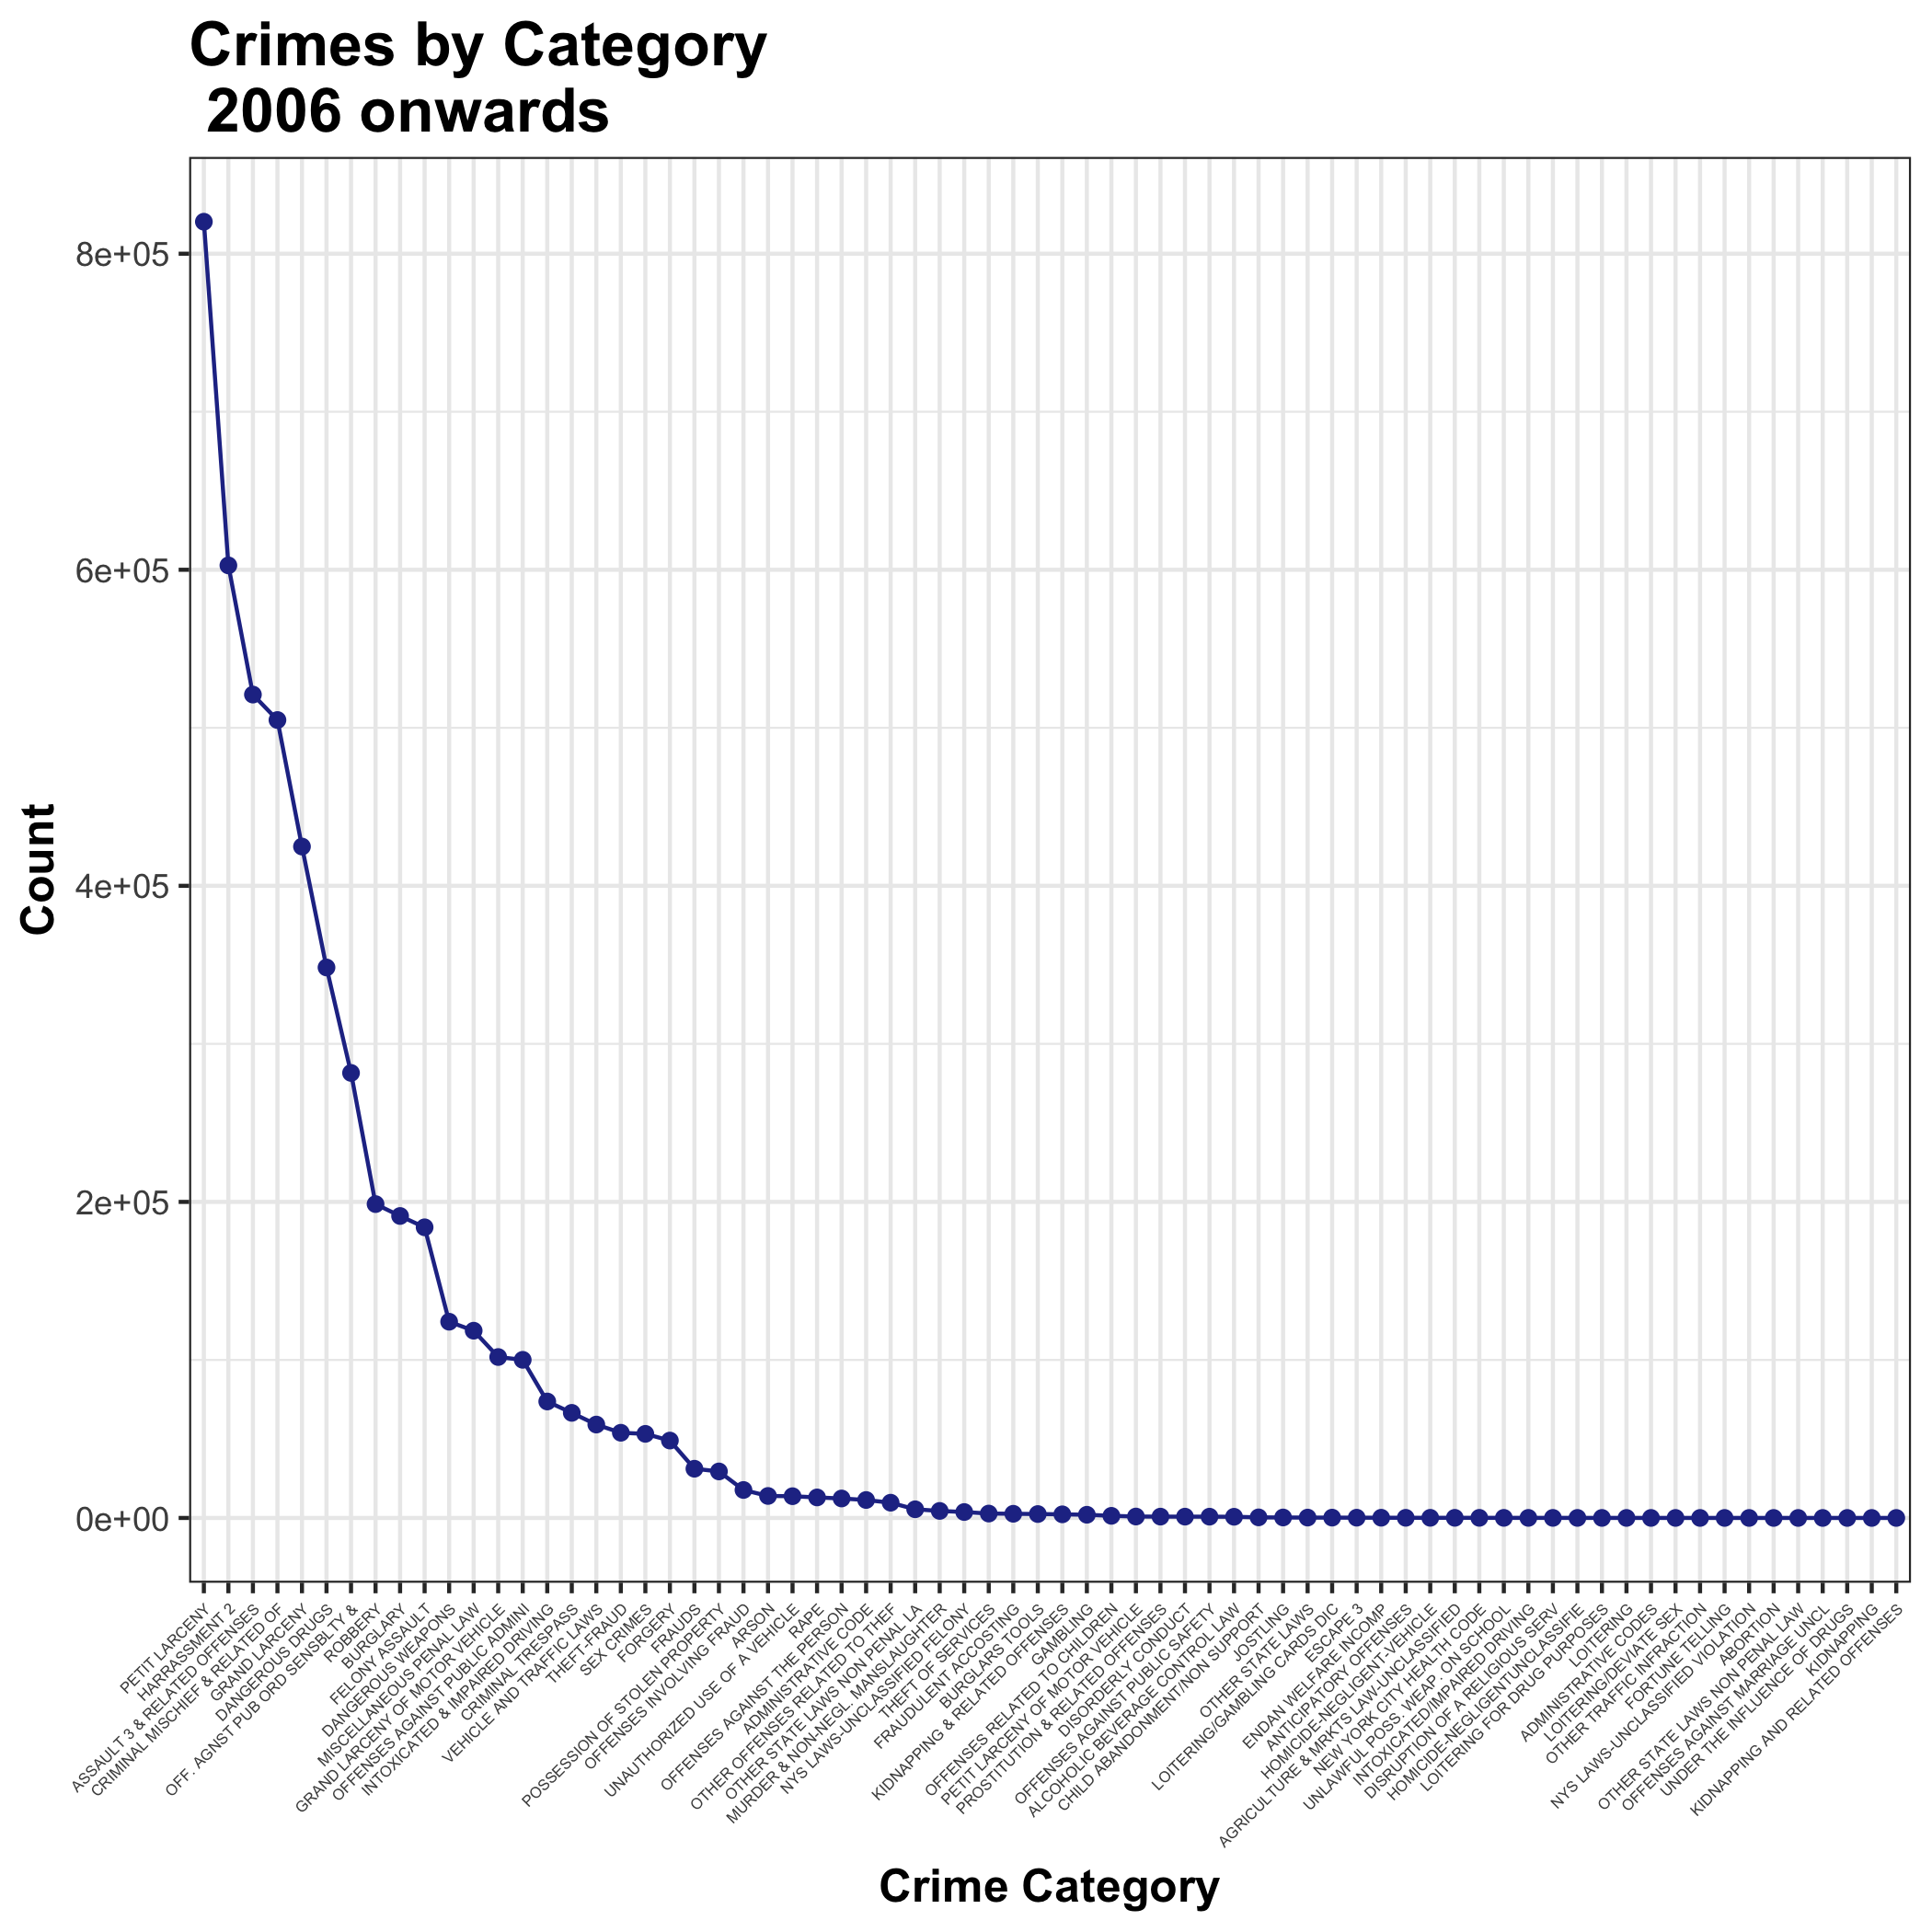
\includegraphics[scale=0.16]{6_Type.png}
\end{figure}

\begin{figure}[H]
\centering
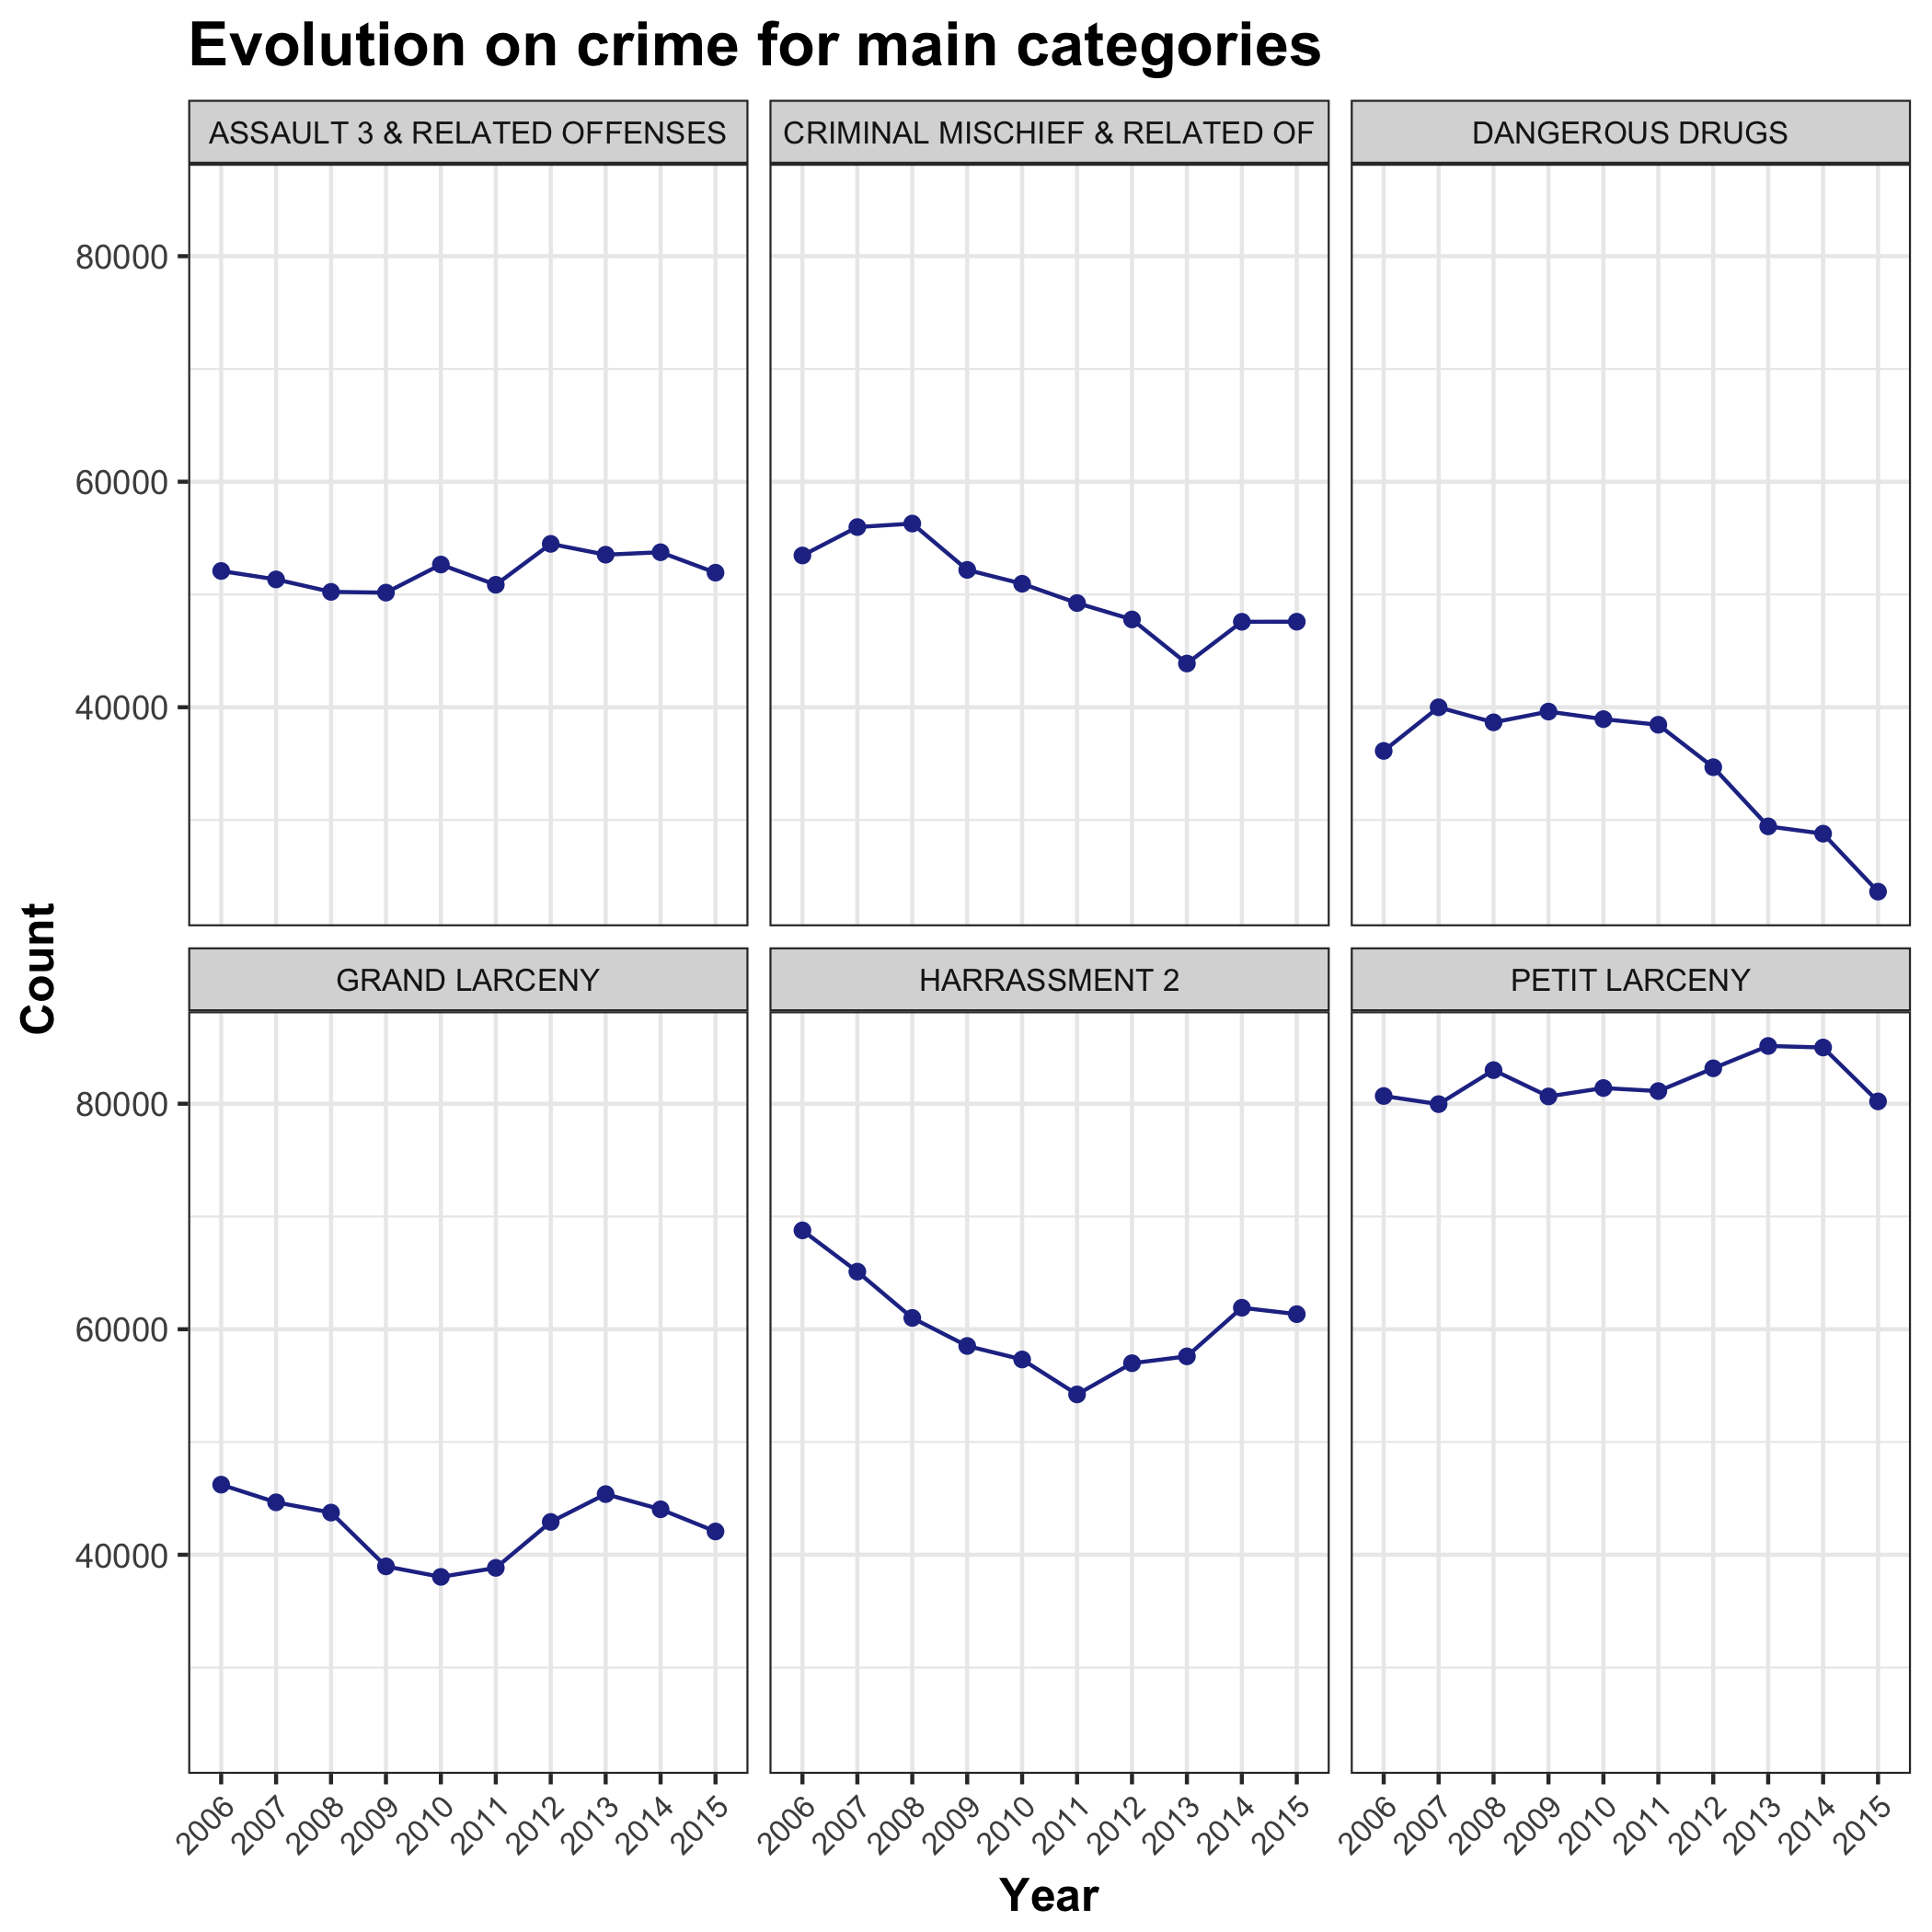
\includegraphics[scale=0.15]{7_MainCatsOverTime.png}
\end{figure}

\pagebreak
\section{Part II: Data Exploration}
\subsection{Sociodemographic characteristics}

\subsubsection{Motivation}

Consider the following graphs demonstrating crime rate across different years.

\begin{figure}[H]
\centering
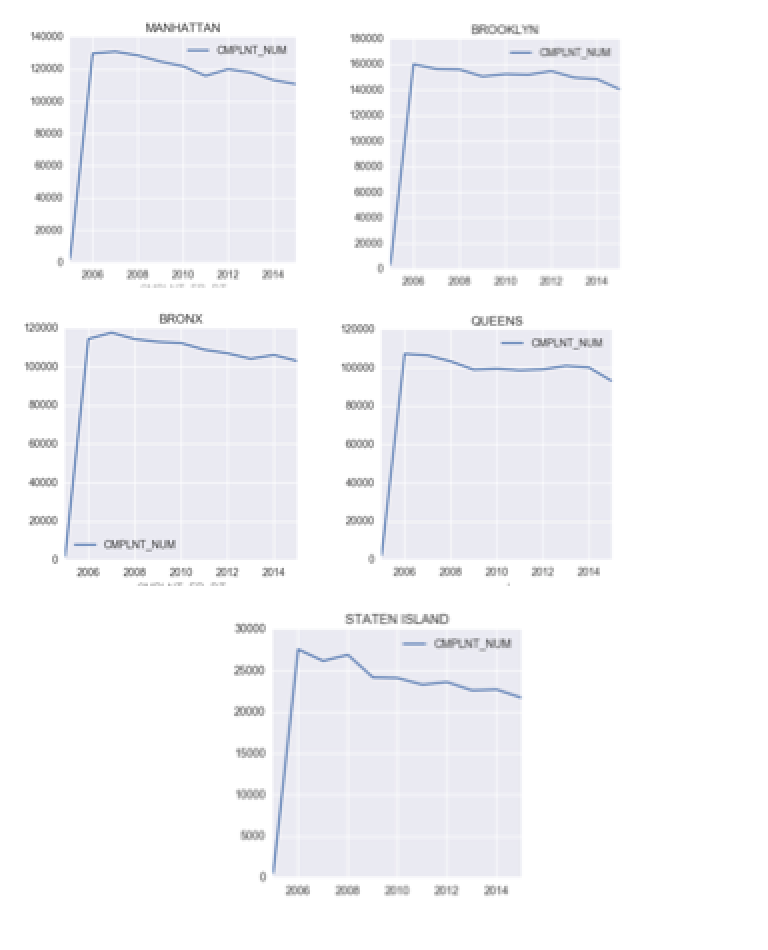
\includegraphics[scale=1]{Akash1.png}
\end{figure}

The crime in New York seems to be following a very linear trend across years from 2006 - 2015. We are not considering years before that, because the graph is highly skewed and looks suspiciously negligible for years before 2006. Since the crime is linearly going down, it certainly makes sense to model this performance with some of the inherent characteristics of the Borough. Some of them could be using features like, total population, Population under poverty, Population of Black people, Percentage of educated people, immigrant’s migration rate, etc. 

In this task, we will try to compare crime rate with some of the above features individually. Our proposed hypothesis is that, the crime rate positively correlates with the features mentioned above.

\subsubsection{Data}

The census data was collected from American FactFinder site. The data being used was prepared by American Community Survey, which uses 1 year estimates to come up with census data.

The 10 csv files (each for a given year), was downloaded individually and then merged into one csv file. This entire csv file was then loaded to pyspark to check for data quality and issues. Note that the data has only 55 rows (5 boroughs * 10 years ). The entire code for data quality and results have been included below.

You could see that the data is clean and no issues have been found. We will use this data for testing our hypothesis. Note that the code is attached in github repo.

\subsubsection*{Results from Data Quality issues for this data}

\begin{minted}{python}
# Data exploration using Pyspark
# PART I
# Validity per column & integrity. 

demographic_csv.count()
# >>> 56

# The count should be 55 (11 years data for 5 boroughs). The extra count is for the column names


##### 1. DATA QUALITY CHECK

### COLUMN 1 - YEAR:

# All the distinct values should be between 2005 and 2015. Hence it should be 11

+----+
|Year|
+----+
|2012|
|2014|
|2013|
|2005|
|2009|
|2006|
|2011|
|2008|
|2007|
|2015|
|2010|
+----+


+--------------------+
|count(DISTINCT Year)|
+--------------------+
|                  11|
+--------------------+


### COLUMN 2 - Borough

# there should be 5 distinct values

+-------------+
|      Borough|
+-------------+
|       Queens|
|     Brooklyn|
|Staten Island|
|    Manhattan|
|        Bronx|
+-------------+


spark.sql("SELECT COUNT (DISTINCT Borough) FROM df").show()

+-----------------------+
|count(DISTINCT Borough)|
+-----------------------+
|                      5|
+-----------------------+


### COLUMN 3 - Total population

# check count - should be 55

spark.sql("SELECT COUNT (Total_population) FROM df").show()

+-----------------------+
|count(Total_population)|
+-----------------------+
|                     55|
+-----------------------+


# Check if it is integer or not

spark.sql("SELECT Total_population ,'integer' AS base_type ,'total population' \
AS semantic_type, CASE WHEN Total_population = '' THEN 'null' \
WHEN Total_population \ 
not LIKE '%[^0-9]%' THEN 'valid' ELSE 'invalid' END AS is_valid from df").show()

+----------------+---------+----------------+--------+
|Total_population|base_type|   semantic_type|is_valid|
+----------------+---------+----------------+--------+
|         1300331|  integer|total population|   valid|
|         2440413|  integer|total population|   valid|
|         1526982|  integer|total population|   valid|
|         2208518|  integer|total population|   valid|
|          454610|  integer|total population|   valid|
|         1320591|  integer|total population|   valid|
|         2485425|  integer|total population|   valid|
|         1565250|  integer|total population|   valid|
|         2230432|  integer|total population|   valid|
|          468646|  integer|total population|   valid|
|         1337923|  integer|total population|   valid|
|         2508282|  integer|total population|   valid|
|         1584449|  integer|total population|   valid|
|         2248820|  integer|total population|   valid|
|          469575|  integer|total population|   valid|
|         1349428|  integer|total population|   valid|
|         2538724|  integer|total population|   valid|
|         1592904|  integer|total population|   valid|
|         2269435|  integer|total population|   valid|
|          478849|  integer|total population|   valid|
+----------------+---------+----------------+--------+


spark.sql("SELECT is_valid, count(is_valid) \  
from (SELECT Total_population ,'integer' \  
AS base_type ,'total population' \  
AS semantic_type, CASE WHEN Total_population = '' \  
THEN 'null' WHEN Total_population \  
not LIKE '%[^0-9]%' THEN 'valid' ELSE 'invalid' END AS is_valid from df) group by is_valid").show()

+--------+---------------+
|is_valid|count(is_valid)|
+--------+---------------+
|   valid|             55|
+--------+---------------+



### COLUMN 4 - Below poverty level


# Check count

spark.sql("SELECT COUNT (Below_poverty_level) FROM df").show()

+--------------------------+
|count(Below_poverty_level)|
+--------------------------+
|                        55|
+--------------------------+

# Check it is integer or not

spark.sql("SELECT Below_poverty_level ,'integer' \  
AS base_type ,'Below_poverty_level' AS semantic_type, CASE \  
WHEN Below_poverty_level = '' THEN 'null' WHEN Below_poverty_level \  
not LIKE '%[^0-9]%' THEN 'valid' ELSE 'invalid' END AS is_valid from df").show()

+-------------------+---------+-------------------+--------+
|Below_poverty_level|base_type|      semantic_type|is_valid|
+-------------------+---------+-------------------+--------+
|             379959|  integer|Below_poverty_level|   valid|
|             545611|  integer|Below_poverty_level|   valid|
|             272890|  integer|Below_poverty_level|   valid|
|             263701|  integer|Below_poverty_level|   valid|
|              49951|  integer|Below_poverty_level|   valid|
|             383788|  integer|Below_poverty_level|   valid|
|             561548|  integer|Below_poverty_level|   valid|
|             286800|  integer|Below_poverty_level|   valid|
|             271980|  integer|Below_poverty_level|   valid|
|              43036|  integer|Below_poverty_level|   valid|
|             362062|  integer|Below_poverty_level|   valid|
|             550169|  integer|Below_poverty_level|   valid|
|             279522|  integer|Below_poverty_level|   valid|
|             270066|  integer|Below_poverty_level|   valid|
|              45877|  integer|Below_poverty_level|   valid|
|             371971|  integer|Below_poverty_level|   valid|
|             536474|  integer|Below_poverty_level|   valid|
|             268635|  integer|Below_poverty_level|   valid|
|             275652|  integer|Below_poverty_level|   valid|
|              47752|  integer|Below_poverty_level|   valid|
+-------------------+---------+-------------------+--------+


# Check for invalid values

spark.sql("SELECT is_valid, count(is_valid) from \  
(SELECT Below_poverty_level ,'integer' AS base_type ,'Below_poverty_level' AS semantic_type, CASE \  
WHEN Below_poverty_level = '' THEN 'null' WHEN Below_poverty_level \  
not LIKE '%[^0-9]%' THEN 'valid' ELSE 'invalid' END AS is_valid from df) group by is_valid").show()

+--------+---------------+
|is_valid|count(is_valid)|
+--------+---------------+
|   valid|             55|
+--------+---------------+


### COLUMN 5 - Percent below poverty level

# Check count

spark.sql("SELECT COUNT (Percent_Below_poverty_level) FROM df").show()

+----------------------------------+
|count(Percent_Below_poverty_level)|
+----------------------------------+
|                                55|
+----------------------------------+


# check the min and max. 
# The min and max should be between 0 and 100 (because it is percentage calculation)


spark.sql("SELECT MIN(int(Percent_Below_poverty_level)) FROM df").show()

+--------------------------------------------------------------------+
|min(CAST(CAST(Percent_Below_poverty_level AS DECIMAL(20,0)) AS INT))|
+--------------------------------------------------------------------+
|                                                                   9|
+--------------------------------------------------------------------+

spark.sql("SELECT MAX(int(Percent_Below_poverty_level)) FROM df").show()

+--------------------------------------------------------------------+
|max(CAST(CAST(Percent_Below_poverty_level AS DECIMAL(20,0)) AS INT))|
+--------------------------------------------------------------------+
|                                                                  32|
+--------------------------------------------------------------------+


# Check it is integer or not

spark.sql("SELECT Percent_Below_poverty_level ,'integer' \  
AS base_type ,'Percent Below poverty level' \  
AS semantic_type, CASE WHEN Percent_Below_poverty_level = '' \  
THEN 'null' WHEN Percent_Below_poverty_level \  
not LIKE '%[^0-9]%' THEN 'valid' ELSE 'invalid' END AS is_valid from df").show()

+---------------------------+---------+--------------------+--------+
|Percent_Below_poverty_level|base_type|       semantic_type|is_valid|
+---------------------------+---------+--------------------+--------+
|                       29.2|  integer|Percent Below pov...|   valid|
|                       22.4|  integer|Percent Below pov...|   valid|
|                       17.9|  integer|Percent Below pov...|   valid|
|                       11.9|  integer|Percent Below pov...|   valid|
|                       11.0|  integer|Percent Below pov...|   valid|
|                       29.1|  integer|Percent Below pov...|   valid|
|                       22.6|  integer|Percent Below pov...|   valid|
|                       18.3|  integer|Percent Below pov...|   valid|
|                       12.2|  integer|Percent Below pov...|   valid|
|                        9.2|  integer|Percent Below pov...|   valid|
|                       27.1|  integer|Percent Below pov...|   valid|
|                       21.9|  integer|Percent Below pov...|   valid|
|                       17.6|  integer|Percent Below pov...|   valid|
|                       12.0|  integer|Percent Below pov...|   valid|
|                        9.8|  integer|Percent Below pov...|   valid|
|                       27.6|  integer|Percent Below pov...|   valid|
|                       21.1|  integer|Percent Below pov...|   valid|
|                       16.9|  integer|Percent Below pov...|   valid|
|                       12.1|  integer|Percent Below pov...|   valid|
|                       10.0|  integer|Percent Below pov...|   valid|
+---------------------------+---------+--------------------+--------+


# Check for invalid values

spark.sql("SELECT is_valid, count(is_valid) \  
from (SELECT Percent_Below_poverty_level ,'integer' \  
AS base_type ,'Percent_Below_poverty_level' \  
AS semantic_type, CASE \  
WHEN Percent_Below_poverty_level = '' THEN 'null' \  
WHEN Percent_Below_poverty_level not LIKE '%[^0-9]%' \  
THEN 'valid' ELSE 'invalid' END AS is_valid from df) group by is_valid").show()


+--------+---------------+
|is_valid|count(is_valid)|
+--------+---------------+
|   valid|             55|
+--------+---------------+


### COLUMN 5 - Percent Below poverty level Black

# Check count

spark.sql("SELECT COUNT (Percent_Below_poverty_level_Black) FROM df").show()

+----------------------------------------+
|count(Percent_Below_poverty_level_Black)|
+----------------------------------------+
|                                      55|
+----------------------------------------+


# check the min and max. 
# The min and max should be between 0 and 100 (because it is percentage calculation)

spark.sql("SELECT MAX(int(Percent_Below_poverty_level_Black)) FROM df").show()

+--------------------------------------------------------------------------+
|max(CAST(CAST(Percent_Below_poverty_level_Black AS DECIMAL(20,0)) AS INT))|
+--------------------------------------------------------------------------+
|                                                                        35|
+--------------------------------------------------------------------------+

spark.sql("SELECT MIN(int(Percent_Below_poverty_level_Black)) FROM df").show()

+--------------------------------------------------------------------------+
|min(CAST(CAST(Percent_Below_poverty_level_Black AS DECIMAL(20,0)) AS INT))|
+--------------------------------------------------------------------------+
|                                                                        11|
+--------------------------------------------------------------------------+


# Check it is integer or not

spark.sql("SELECT Percent_Below_poverty_level_Black ,'integer' \  
AS base_type ,'Percent_Below_poverty_level_Black' AS semantic_type, CASE \  
WHEN Percent_Below_poverty_level_Black = '' THEN 'null' \  
WHEN Percent_Below_poverty_level_Black not LIKE '%[^0-9]%' \  
THEN 'valid' ELSE 'invalid' END AS is_valid from df").show()

+---------------------------------+---------+--------------------+--------+
|Percent_Below_poverty_level_Black|base_type|       semantic_type|is_valid|
+---------------------------------+---------+--------------------+--------+
|                             26.3|  integer|Percent_Below_pov...|   valid|
|                             21.1|  integer|Percent_Below_pov...|   valid|
|                             30.0|  integer|Percent_Below_pov...|   valid|
|                             11.9|  integer|Percent_Below_pov...|   valid|
|                             30.6|  integer|Percent_Below_pov...|   valid|
|                             27.1|  integer|Percent_Below_pov...|   valid|
|                             23.2|  integer|Percent_Below_pov...|   valid|
|                             31.7|  integer|Percent_Below_pov...|   valid|
|                             11.9|  integer|Percent_Below_pov...|   valid|
|                             22.7|  integer|Percent_Below_pov...|   valid|
|                             24.2|  integer|Percent_Below_pov...|   valid|
|                             20.9|  integer|Percent_Below_pov...|   valid|
|                             29.8|  integer|Percent_Below_pov...|   valid|
|                             11.3|  integer|Percent_Below_pov...|   valid|
|                             27.2|  integer|Percent_Below_pov...|   valid|
|                             25.1|  integer|Percent_Below_pov...|   valid|
|                             20.9|  integer|Percent_Below_pov...|   valid|
|                             28.7|  integer|Percent_Below_pov...|   valid|
|                             12.3|  integer|Percent_Below_pov...|   valid|
|                             31.9|  integer|Percent_Below_pov...|   valid|
+---------------------------------+---------+--------------------+--------+


# Check for invalid values

spark.sql("SELECT is_valid, count(is_valid) \  
from (SELECT Percent_Below_poverty_level_Black ,'integer' \  
AS base_type ,'Percent_Below_poverty_level_Black' AS semantic_type, CASE \  
WHEN Percent_Below_poverty_level_Black = '' \  
THEN 'null' WHEN Percent_Below_poverty_level_Black \  
not LIKE '%[^0-9]%' THEN 'valid' ELSE 'invalid' \  
END AS is_valid from df) group by is_valid").show()

+--------+---------------+
|is_valid|count(is_valid)|
+--------+---------------+
|   valid|             55|
+--------+---------------+

### COLUMN 6 - Percent with education less than high school level 

# Check count

spark.sql("SELECT COUNT (Percent_Below_poverty_level_Black) FROM df").show()

+----------------------------------------+
|count(Percent_Below_poverty_level_Black)|
+----------------------------------------+
|                                      55|
+----------------------------------------+


# check the min and max. 
#The min and max should be between 0 and 100 (because it is percentage calculation)

spark.sql("SELECT MIN(int(percent_with_education_below_high_school)) FROM df").show()

spark.sql("SELECT MAX(int(percent_with_education_below_high_school) FROM df").show()

# Check it is integer or not

spark.sql("SELECT percent_with_education_below_high_school ,'integer' \  
AS base_type ,'percent_with_education_below_high_school' \  
AS semantic_type, CASE WHEN percent_with_education_below_high_school = '' \ 
THEN 'null' WHEN percent_with_education_below_high_school \  
not LIKE '%[^0-9]%' THEN 'valid' ELSE 'invalid' END AS is_valid from df").show()

# Check for invalid values

spark.sql("SELECT is_valid, count(is_valid) from (SELECT percent_with_education_below_high_school ,'integer' \  
AS base_type ,'percent_with_education_below_high_school' \  
AS semantic_type, CASE \  
WHEN percent_with_education_below_high_school = '' THEN 'null' \  
WHEN percent_with_education_below_high_school \  
not LIKE '%[^0-9]%' THEN 'valid' ELSE 'invalid' END AS is_valid from df) group by is_valid").show()
\end{minted}

\subsubsection{Experimental techniques and methods}

To prove our hypothesis we need to check the dependence of features with the crime rate in New York. Hence, we will be testing the correlation of each feature with the crime rate. For this we will be using the "Statistics" library of pyspark. 

For checking correlation, we would be using the Pearson correlation measure. It is calculated as coefficient is the covariance of the two variables divided by the product of their standard deviations. The form of the definition involves a "product moment", that is, the mean (the first moment about the origin) of the product of the mean-adjusted random variables. It is equal to $$\rho(X,Y) = \frac{{\bf
Cov}(X,Y)}{\sqrt{{\bf Var}(X){\bf Var}(Y)}}.$$

Apart from this, we will be doing visualization of these features across years, and compare them the trend of crime rate. 

The results of our analysis is shown below.

\subsubsection{Results}
\subsubsection*{Part – I: (Checking correlation)}

For this section, Pearson correlation of mllib library was used. The code and results of this is (using pyspark) :

\begin{minted}{python}
# Finding correlation

v1 = demographic_csv.map(lambda x: x[3]) # vector for total population
v2 = demographic_csv.map(lambda x: x[4]) # vector for population under poverty level
v3 = demographic_csv.map(lambda x: x[14]) # vector for black population
v4 = demographic_csv.map(lambda x: x[20]) # vector for under-educated population
v5 = demographic_csv.map(lambda x: x[19]) # Total crime count

# Correlation between total population and crime count
print("Correlation is: " + str(Statistics.corr(v1, v5, method="pearson")))
# Correlation is: 0.6767118210127591

# Correlation between population under poverty level and crime count
print("Correlation is: " + str(Statistics.corr(v2, v5, method="pearson")))
# Correlation is: 0.7305919332530579

# Correlation between black population and crime count
print("Correlation is: " + str(Statistics.corr(v3, v5, method="pearson")))
# Correlation is: 0.6712880230552578


# Correlation between under-educated population and crime count
print("Correlation is: " + str(Statistics.corr(v4, v5, method="pearson")))
# Correlation is: 0.6321731661199721
\end{minted}

From the above results, we see that every feature seem to be statistically significant since they have more than 60\% of correlation with the crime rate. This proves a part of our hypothesis. Next we will visualize each feature and see how it compares with the distribution of crime.

\subsubsection*{Part – II: Visualizing the graphs for features and comparing them}
\begin{itemize}
\item Manhattan (New York County)
\begin{enumerate}[label=(\alph*)]
\item POPULATION

\begin{figure}[H]
\centering
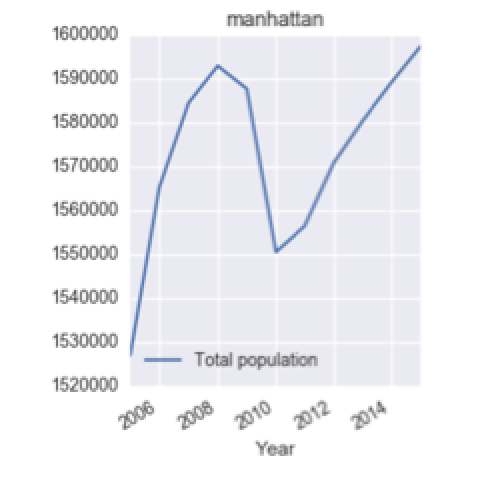
\includegraphics[scale=1]{ManhattanPopulation.png}
\end{figure}

We see that the population of Manhattan drops substantially in the year 2010, and then starts to increase slowly. Also, we know that the crime data calculated for the year 2011 uses the data uptil 2010. Hence, population seems to have a direct correlation with crime. 

\item POPULATION UNDER POVERTY LEVEL

\begin{figure}[H]
\centering
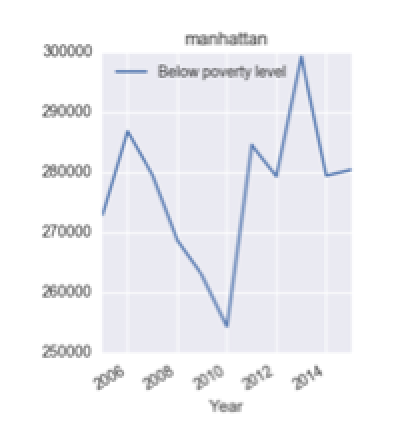
\includegraphics[scale=1]{ManhattanPoverty.png}
\end{figure}

We see that the percent of population of people living under poverty is less in the year 2011. This might be clear from the fact that population in 2011 was less (as shown in the graph above). 

This measure also has a positive correlation for predicting crime rate in Manhattan.

\item POPULATION OF BLACK PEOPLE

\begin{figure}[H]
\centering
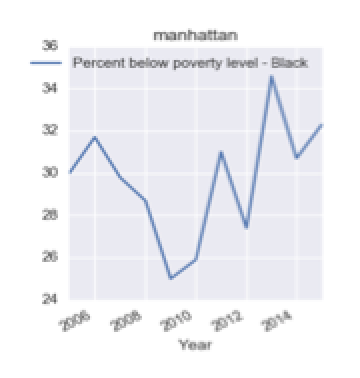
\includegraphics[scale=1]{ManhattanBlack.png}
\end{figure}

We did try to visualize graph of different races vs the crime rate. Only the population of black people seemed to have a positive correlation. The graph is attached below. 

We witness that this feature also seems to drop around the year 2010 and then increases. Almost similar trend is being followed by crime rate.

\item EDUCATIONAL ATTAINMENT LEVEL FOR PEOPLE OVER 25 YEARS

\begin{figure}[H]
\centering
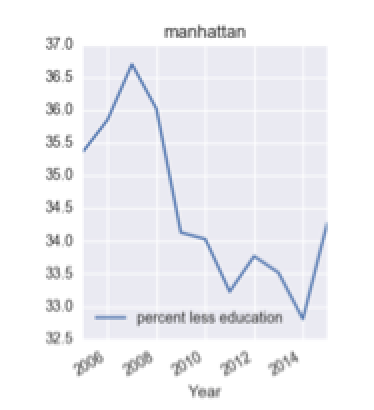
\includegraphics[scale=1]{ManhattanEduc.png}
\end{figure}

Even this complements the behavior of crime rates in manhattan. We see that the maximum number of people with less education level is in 2006 and minimum is during the years 2013 and 2014. Correspondingly, we will expect the crimes rates reported at the end of year 2006 to be high and those reported during the years 2013 and 2014 to be least. This is clearly true from the crime distribution graph of Manhattan. 

Hence the hypothesis framed for the relation between crime and general demographic data is clearly valid for Manhattan.
\end{enumerate}

\item Brooklyn (King's County)

\begin{enumerate}[label=(\alph*)]

\item POPULATION

\begin{figure}[H]
\centering
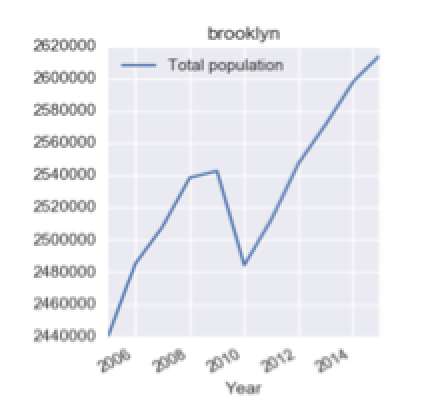
\includegraphics[scale=1]{BrooklynPopulation.png}
\end{figure}

We see that the population of Brooklyn increases linearly uptil the year 2008 and then starts dropping substantially for the years 2009 and 2010, which explains for the slight decrease in crime rate. It then increases sharply and becomes maximum in the year 2015. Unfortunately, crime rate is least as opposed to being high with increasing population. This might be due to other factors like decreased uneducated population level as shown below.

\item POPULATION UNDER POVERTY LEVEL

\begin{figure}[H]
\centering
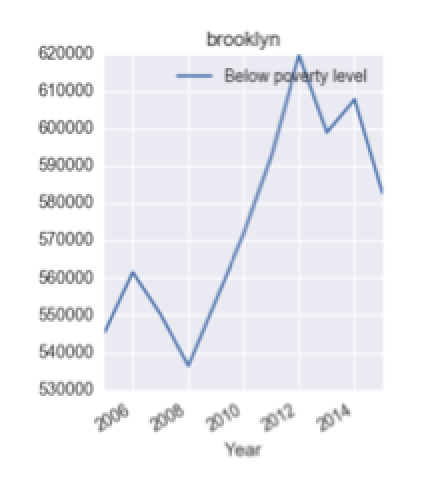
\includegraphics[scale=1]{BrooklynPoverty.png}
\end{figure}

We see that the percent of population of people living under poverty is less in the years 2009 and 2015, which unsurprisingly are also the years with less crimes. Relatively, it is higher in the year 2012 and then in 2006. This can account for almost same number of crimes in those years. Also, this population starts decreasing towards the end of 2014, and so does the crime rate.

\item POPULATION OF BLACK PEOPLE

\begin{figure}[H]
\centering
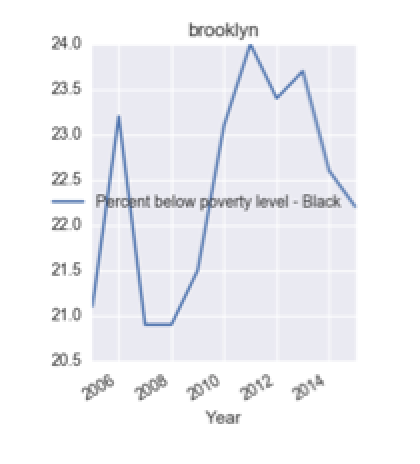
\includegraphics[scale=1]{BrooklynBlack.png}
\end{figure}

Almost similar trend is being followed by the percent of black population in Brooklyn. The trend starts to decrease (and so as crime rate) and then increases with increasing crime rate.

\item EDUCATIONAL ATTAINMENT LEVEL FOR PEOPLE OVER 25 YEARS

\begin{figure}[H]
\centering
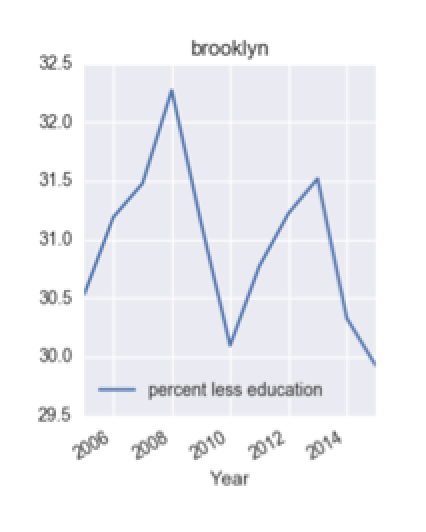
\includegraphics[scale=1]{BrooklynEduc.png}
\end{figure}

Even this measure complements the behavior of crime rates in Brooklyn. We see that the maximum number of people with education level is in 2009 and minimum is during the year 2015. Correspondingly, the crimes rates reported at the end of year 2009 to be high and those reported during the year 2014 to be least. This latter is clearly true from the crime distribution graph of brooklyn, but the former is not. This is because, the population in 2009 was very less as compared to other years in brooklyn. Hence, the total number of people with less education should also be less, which explains less crime. 

The graph for other boroughs have also been shown below. We can see that the hypothesis seems to be valid for every one of them, which also explains the high correlation value of every feature with the crime rate.
\end{enumerate}

\item  BRONX (BRONX COUNTY)
\begin{enumerate}[label=(\alph*)]

\item POPULATION

\begin{figure}[H]
\centering
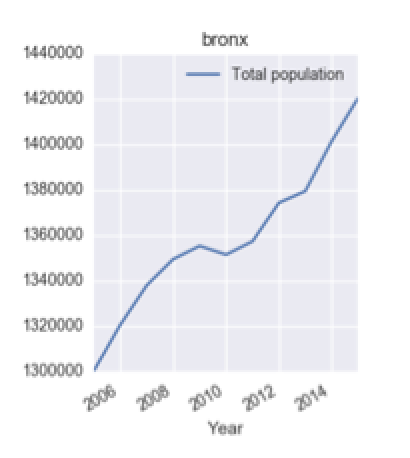
\includegraphics[scale=1]{BronxPopulation.png}
\end{figure}

Even though population seems to increasing, surprisingly crime rate decreases. Hence other features might be useful apart from this.

\item POPULATION UNDER POVERTY LEVEL

\begin{figure}[H]
\centering
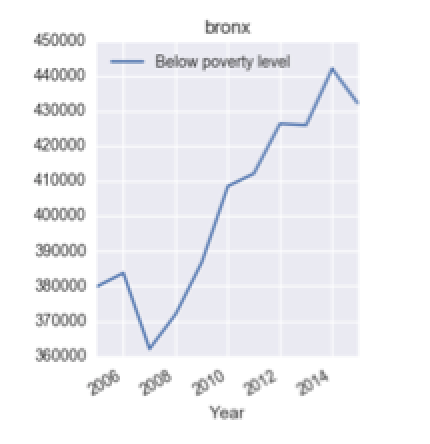
\includegraphics[scale=1]{BronxPoverty.png}
\end{figure}

Here we see that the relationship is almost dissimilar. This can be because, population and population under poverty are directly correlated. Hence, still seeing other features is better

\item POPULATION OF BLACK PEOPLE

\begin{figure}[H]
\centering
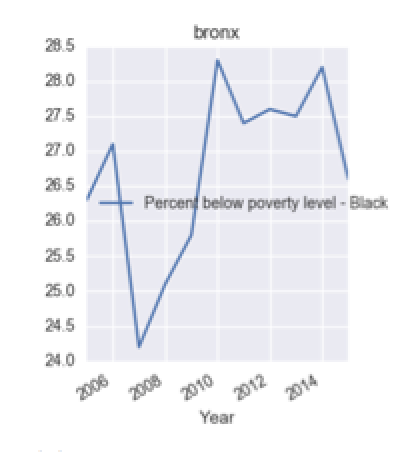
\includegraphics[scale=1]{BronxBlack.png}
\end{figure}

Here we see that relationship is is almost constant initially and then decreases. This is almost the distribution of crime in Bronx. 

\item EDUCATIONAL ATTAINMENT LEVEL FOR PEOPLE OVER 25 YEARS

\begin{figure}[H]
\centering
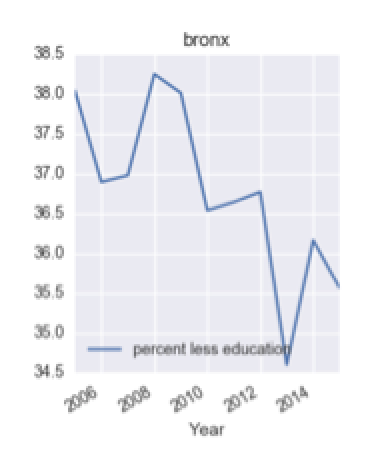
\includegraphics[scale=1]{BronxEduc.png}
\end{figure}

This is clearly 100\% correlated with crime in Bronx if you examine both these graphs. Hence, in Bronx, Education count rally plays a major role to determine crime rate.
\end{enumerate}

\item QUEENS (QUEENS COUNTY)

\begin{enumerate}[label=(\alph*)]

\item POPULATION

\begin{figure}[H]
\centering
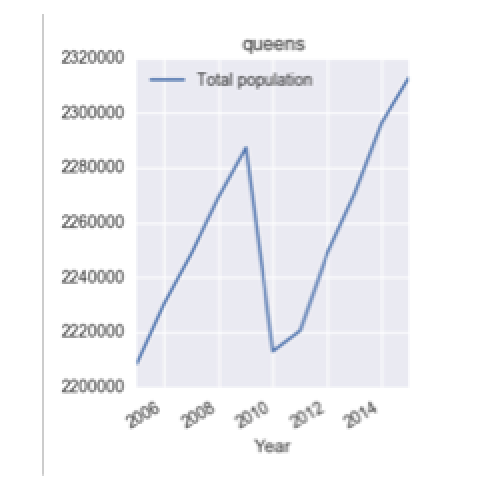
\includegraphics[scale=1]{QueensPopulation.png}
\end{figure}

The population is fairly the same with slight increases and decrease. It is also the case for crime distribution.

\item POPULATION UNDER POVERTY LEVEL

\begin{figure}[H]
\centering
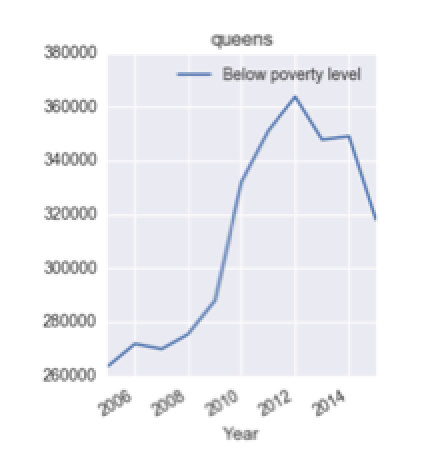
\includegraphics[scale=1]{QueensPoverty.png}
\end{figure}

Here we see that poverty level increases towards the end and so does crime.

\item POPULATION OF BLACK PEOPLE

\begin{figure}[H]
\centering
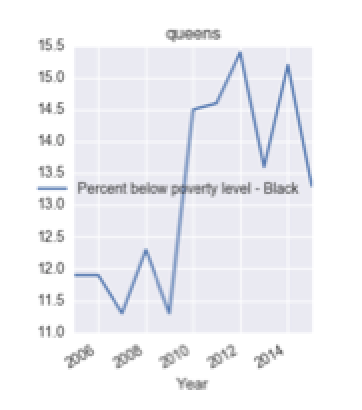
\includegraphics[scale=1]{QueensBlack.png}
\end{figure}

This again, increases towards the end with increasing crime rate. Hence even this measure plays a high significant role.

\item EDUCATIONAL ATTAINMENT LEVEL FOR PEOPLE OVER 25 YEARS

\begin{figure}[H]
\centering
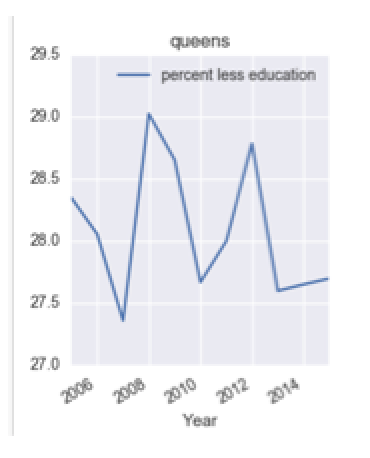
\includegraphics[scale=1]{QueensEduc.png}
\end{figure}

For Queens, percent with less education remained the same across years and it is difficult to measure crime rate with respect to this. But other measures like black population and poverty level population seem to do a pretty good job.
\end{enumerate}

\item STATEN ISLAND (RICHMOND COUNTY)
\begin{enumerate}[label=(\alph*)]

\item POPULATION

\begin{figure}[H]
\centering
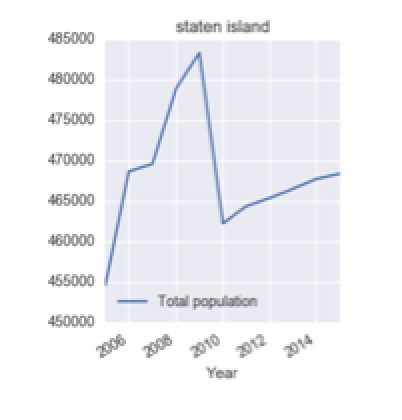
\includegraphics[scale=1]{SIpopulation.png}
\end{figure}

Staten Island crime rate linearly decreases which also is somewhat the case for population across the years.

\item POPULATION UNDER POVERTY LEVEL

\begin{figure}[H]
\centering
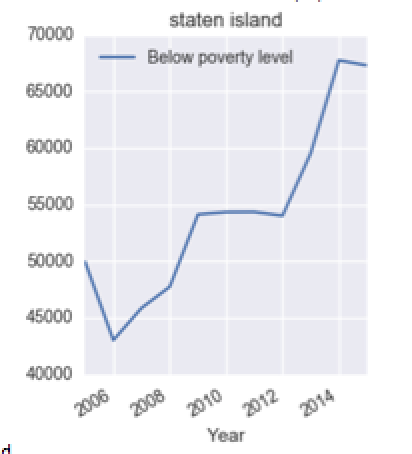
\includegraphics[scale=1]{SIpoverty.png}
\end{figure}

Surprisingly, this measure is highly negative with the crime rate in Staten Island. But other features like education level and black population seem to do better job for Staten Island.

\item POPULATION OF BLACK PEOPLE

\begin{figure}[H]
\centering
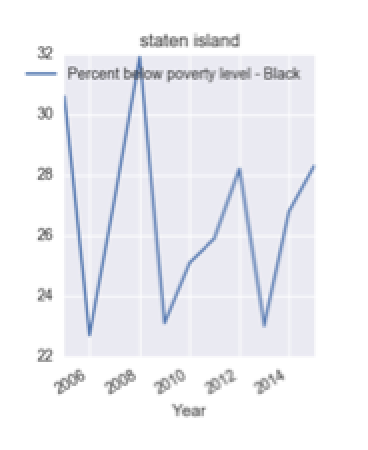
\includegraphics[scale=1]{SIBlack.png}
\end{figure}

As seen from the graph, the population of black people decreases with time, which is also the trend or crime in Staten Island. Hence, it is positively correlated also.

\item EDUCATIONAL ATTAINMENT LEVEL FOR PEOPLE OVER 25 YEARS

\begin{figure}[H]
\centering
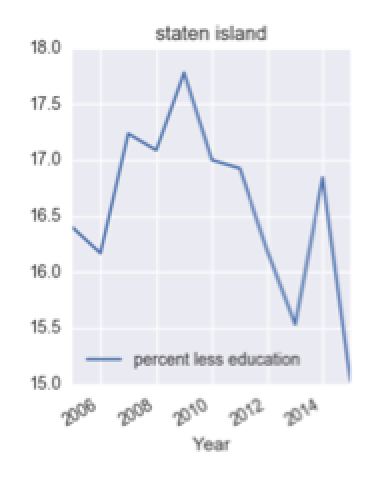
\includegraphics[scale=1]{SIEduc.png}
\end{figure}
\end{enumerate}
\end{itemize}

\subsubsection{Discussion}

From the above-described results, every borough had at least 3 out 4 features to be directly positively correlated with the crime rate. This also explains why the Pearson correlation rate was so high. Hence, using these two results, we can say that the hypothesis that the crime rates vary a lot with general demographic data is sufficiently true. 

The analysis carried out above was based on borough level. The same problem could be done at a much smaller granularity like, observing the crime rate at zip code level, census block level and census tract level. Due to time constraints and data limitations, we could limit our analysis to borough level only. The data limitations were that the data was very inconsistent at these granularity levels. The inconsistencies included the time range of the data (it didn’t cover all the years from 2006 – 2015), and some features missing were missing in some of the years, which made it difficult for us to perform our analysis.

\pagebreak
\subsection{Baseball Games}
\subsubsection{Motivation}
After this general analysis, we decided to try a more \textit{micro} approach, with a more detailed geographic specification, taking advantage on the granularity of the data. One of the most interesting hypothesis that arose is discussing the data was: Do Sport Events affect crime in New York City? To test this, we decided to experiment over the sport with the most number of games in a year whose stadiums are actually inside the city: Baseball. 

Part of this hypothesis was inspired by a work in 2013 in for Mexico and Soccer, where Eduardo Clark ~\autocite{Clark} tested if Soccer games in increases the number of homicides. It's worth noting that by 2011, homicides in Mexico were at a historic high, with a rate of over 24 deaths per 100,000 people. On this context, Eduardo Clark ~\autocite{Clark} showed that ``game days had on average 0.6 more homicides than non game days''. 

This hypothesis for soccer is shared with Nadia Campaniello ~\autocite{Campaniello}, who shows with data from 1990 that ``that hosting the Football World Cup leads to a significant increase in most property crimes (bag-snatching, pickpocketing, shoplifting, and burglary) but only in one violent crime (intentional personal injuries).'' ~\autocite{Campaniello}

On United States, Daniel Rees and Kevin T. Schnepel, using daily offense data from the National Incident-Based Reporting System (NIBRS)  and matching it with 26 College Football Programs, conclude that `` the host community registers sharp increases in assaults, vandalism, arrests for disorderly conduct, and arrests for alcohol-related offenses on game days'' ~\autocite{Rees_Schnepel}.

With this, we landed to a hypothesis: Does the incidence of crime increases around the venue (Citi Field and Yankee Stadium) when there is a baseball game? As a secondary hypothesis, using the same data and results, and taking the first hypothesis as given, we decided to test if there is a difference around the Citi field stadium (Mets) and the Yankee Stadium (Yankees). 

\subsubsection{Data}
The first problem we faced was getting the data. How many games have happened since 2006 (when crime data starts to be reliable according to our previous analysis)? Turns out that although Baseball is one of the sports where more data gets analyzed and with a great data-analysis tradition, non of the websites we visited had a simple and cleaned data-frame we could use. 

Because of this, we decided to scrape the website \textit{http://www.baseball\-reference.com/teams/NYY/2012.shtml}, using \texttt{R}. With this, we got data relating the exact date of the match for the Yankees and the Mets on it's stadiums, plus some other figures as attendance and whether they won or lost. 

Second, we faced the geographic problem. To take advantage of the granularity of the data, we decided to define four different bounding boxes around each of the Baseball stadiums: 250 meters, 500 meters, 1000 meters and 2000 meters. This was also done in \texttt{R}, taking advantage of it's geographic packages \texttt{rgeos} and \texttt{rgdal}, this last based on the GDAL project (http://www.gdal.org/).

\subsubsection{Experimental techniques and methods}
Using the bounding boxes computed above, we decided to test our hypothesis running a bunch of linear regressions for each crime (and all the crimes together) and the day of occurrence for all of the crimes in the bounding boxes described above. This follows the following equation: $$y_{i} = \alpha + \beta x_{i} + \epsilon_{i}.$$ In this equation, $y_{i}$ represents the number of crimes (say, for example, ``OFFENSES INVOLVING FRAUD'') on the predefined bounding box (say, 250 meters bounding box) on day $i$. $\alpha$ represents a constant vector of ones, while $x_{i}$ is a vector of ones and zeros indicating if that day had a baseball game around the stadium (say, for example, Yankee Stadium).  

With this formulation, following the example above. $\beta$ represents the change on ``OFFENSES INVOLVING FRAUD'' when there's a Baseball game compared when there is no baseball game. $\alpha$, on the other hand, represents the mean value of crimes when there is no baseball game, and $\beta$ +  $\alpha$ the mean value when there is a baseball game: 
$$ \beta = \mathbf{E}\left(\text{Crimes when there is a baseball game } -  \text{ Crimes when there is a baseball game}\right)$$
$$\alpha = \mathbf{E}\left(\text{OFFENSES INVOLVING FRAUD } | \text{ There is NO a Baseball Game}\right)$$
$$\beta + \alpha = \mathbf{E}\left(\text{OFFENSES INVOLVING FRAUD } | \text{ There is a Baseball Game}\right)$$

This regressions were tested on the whole data frame, for each of the crimes (plus all the crimes together), the four distances (250 meters, 500 meters, 1000 meters and 2000 meters) and the two stadiums separately (Citi Field and Yankee Stadium). This is, \textbf{a total of 568 linear regressions were tested}, and their results analyzed. 

Using \texttt{pyspark}, we created a number of functions to import and process the data. The first of this, subsets the crime data to the desired bounding box around the stadium (again, predefined with length 250 meters, 500 meters, 1000 meters and 2000 meters). 

The second function, joins the crime data and with the baseball data described above, in order to recognize if the crimes on the bounding box were during a game-day (and which), and on which stadium this happens. Last, the third functions prepares the data for the regression model. 

All this 568 regressions were run using \texttt{pyspark} package \texttt{ml.regression}. Their results are correctly output as a text file, including distance evaluated, crime evaluated, stadium,  $\alpha$, $\beta$ and p-value\footnote{The method .pvalue for LinearRegression on pyspark.ml.regression is, accroding to the web page of the ml package, still experimental. We did encounter many bugs, and had to program pvalue inside of a $try:$ - $except:$ statement}. 

For this analysis, we used spark on \texttt{Dumbo}, NYU's 48-node Hadoop cluster, running Cloudera CDH 5.9.0 (Hadoop 2.6.0 with Yarn)\footnote{For more information: https://wikis.nyu.edu/display/NYUHPC/Clusters+-+Dumbo}. The version of \texttt{pyspark} after configuration on Dumbo is  2.0.0.cloudera1, using Python version 3.4.4. 

Before describing the results, it's worth describing some of the drawbacks we faced while doing this analysis. First of all, because we used the most recent version of the \textit{ml} package for pyspark, the documentation is still very poor, and most of the questions we had about it's usage are not simply already answered in forums as stackoverflow. 

Second, we first begun testing another algorithm: \texttt{LinearRegressionWithSGD}, from the \texttt{mllib} library (which is now, according to it's documentation, now deprecated). We decided to try the newest algorithm mainly because this one outputs intresting information as the pValue. This change represented also a change in the input data that is fed to the model: while \texttt{ml.LinearRegression} requires the user to build the data using \texttt{pyspark}'s \texttt{SQLContext}, \texttt{mllib.LinearRegressionWithSGD} requires the user to build an RDD object using \texttt{LabeledPoint()}. This, apart from changing part of the logic of code, also represented investing time replicating the few examples available for \texttt{ml.LinearRegression}, to figure out how the data is required to be structured to feed it to the model. 

Third, because we automatize the regressions via a for-loop, we faced the problem of asking the algorithm to fit a regression in a not full-rank matrix (i.e., when there were no crimes of the specified type in the specified bounding box, so the matrix was full of zeros). This, naturally, resulted in a \texttt{ValueError} exception, which we had to filtered using a  \texttt{try-except} statement. 

Finally, as already stated, the \texttt{.pValues} method of the algorithm is still in experimental according to the documentation. This forced us to use yet another \texttt{try-except} statement.  

\subsubsection{Results}

\subsubsection*{Difference in crimes per day}

Using all the crimes as a baseline, for any distance around any of the stadiums, there is a statistically significant difference in crimes when there is a game compared to when there are no games: 

\begin{center}
\textbf{Mean difference in daily crimes when there is game VS when there is no game} 
\medskip

\begin{tabular}{ |c|c|c|c| } 
\hline
\textbf{Distance} & \textbf{Stadium} & \textbf{Difference ($\beta$)} & \textbf{pValue} \\
\hline
   2000 & Yankees & 13.510631 & 0\\ 
   1000 & Yankees & 3.833771 & 0\\ 
   2000 & Mets  & 3.273032 & 0\\ 
   500 & Yankees & 1.761743 & 0 \\ 
   500 &   Mets & 1.522684 & 0\\ 
   250 & Yankees & 1.472647 & 0 \\ 
   250 & Mets & 1.412039 & 0\\ 
   1000 & Mets & 1.281720 & 0\\ 
\hline 
\end{tabular}
\end{center}
\medskip

For example, for a 2,000 meters bounding box around the Yankee Stadium, there are on average 13.5 more crimes on days when there is a Baseball game compared to days when there is no baseball game. This is a jump of 88.4 daily crimes 101.983114, statistically different from zero under a 2-tails ttest with a 99\% confidence interval. 

\begin{center}
[SEE MAPS ON APPENDIX I]
\end{center}

Other than the category aggregating all crimes, there are a number of different categories whose daily crimes increase statistically different than zero when there is a game than when there is no game. For example, inside a bounding box of 250 meters, there are 15 other relevant crime categories around the Mets stadium and 26 around Yankee Stadium. This number increase to 16 and 32 for the 500 meters bounding box, 26 and 37 for the 1000 meters and 35 and 47 for the 2000 meters bounding box, respectively. 

\begin{figure}[H]
\centering
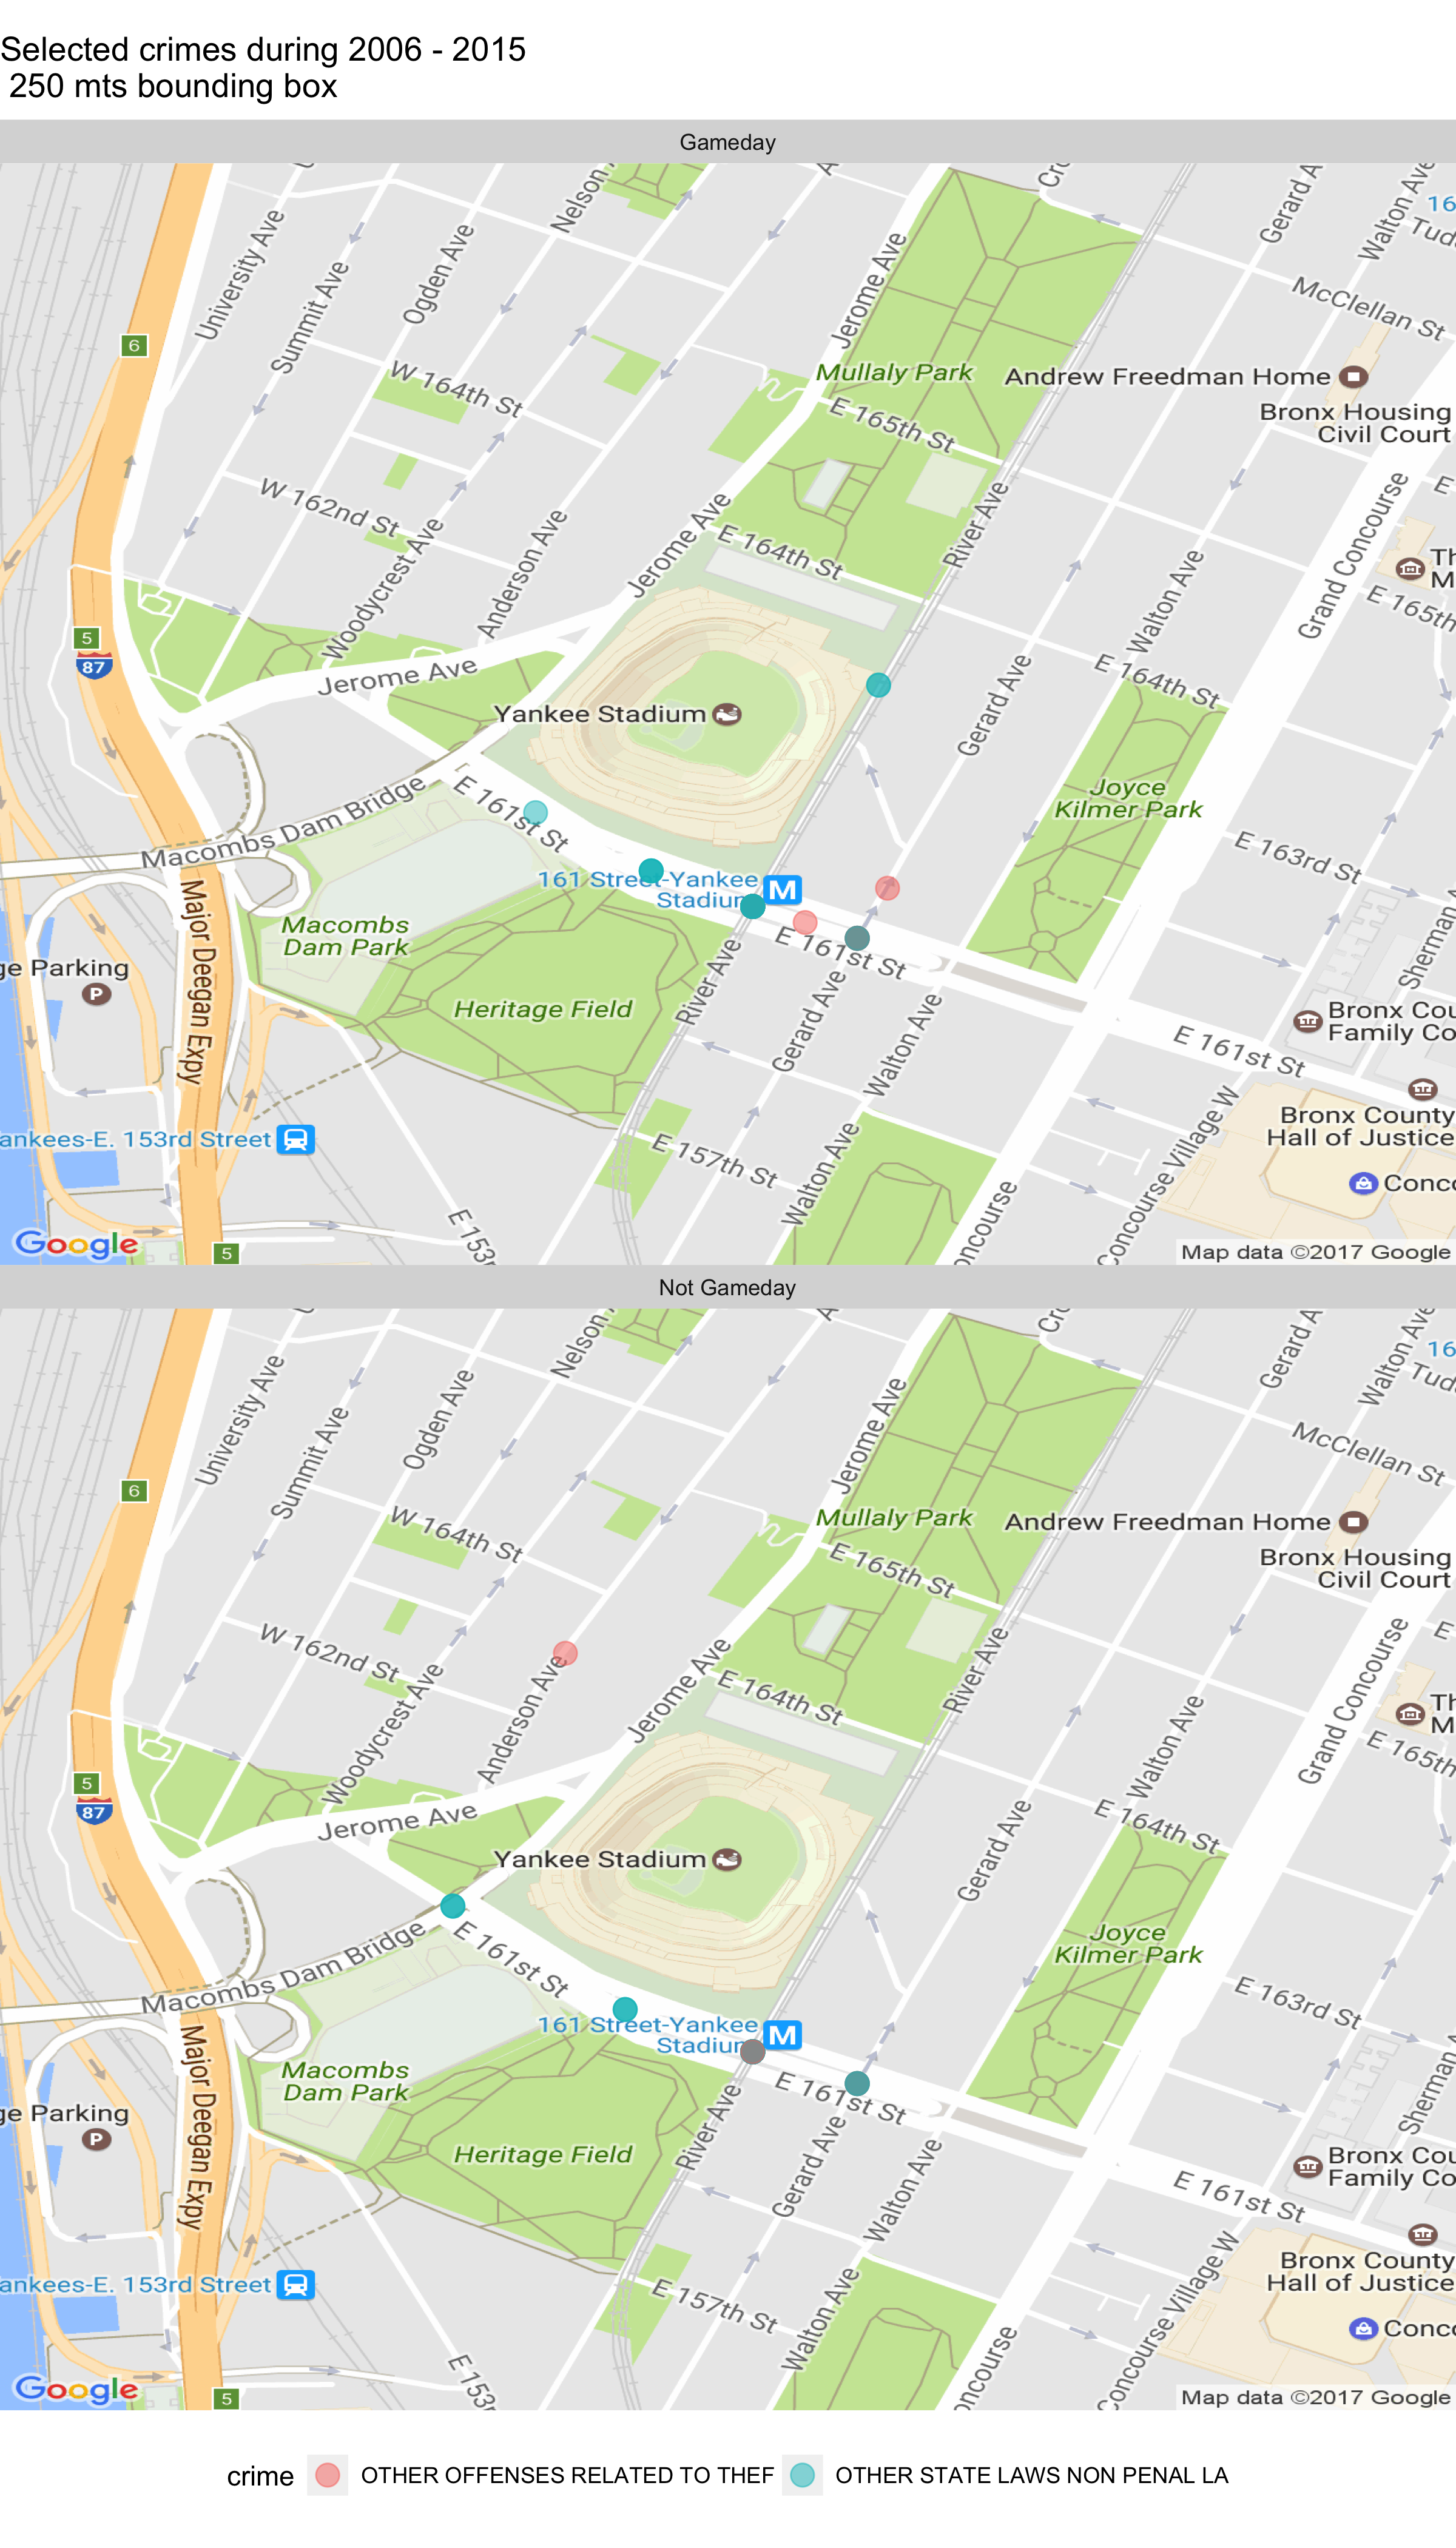
\includegraphics[scale=0.1]{9_YankeesOthers250mts.png}
\end{figure}

To conclude this hypothesis, there is strong evidence to suggest that in fact, crimes increase when there is a Baseball Game than when there is no game. This, of course, is subject to string criticisms and discussion, that will be addressed on the next sub-section.   

\subsubsection*{Game-day crime increase: Yankees vs Mets}

To evaluate the increase of crime when it is a Game-day, we analyzed the estimated coefficients $\beta$ for both stadiums and all crimes. It is important to note that the regression outputs where initially filtered to get rid of invalid p-values, this discarded some models. Additionally, to increase the confidence in the results presented, we focused only on crimes where the estimated coefficients are significant for all four distances from the stadium. For significant coefficients the associated p-value is less than 0.05. 

To begin the comparison, we compared the distribution of the $\beta$ coefficient between the Yankees and the Mets stadium. This initial approach studies all distances and crimes combined, and our variable indicates the increase in the mean of crimes per day. 

\begin{figure}[H]
\centering
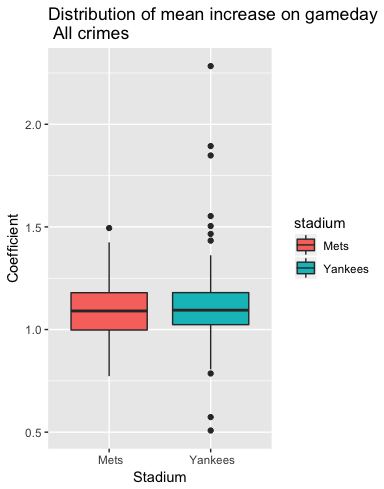
\includegraphics[scale=0.5]{box_1.png}
\end{figure}

From the box plot it is not immediate to  tell if there is a difference in the distribution of the crime increase. The means for both stadiums seem to be at the same level and besides the fact that there is more variance for the coefficients from the Yankee's stadium, there is no evident difference in the distributions. 

The next step is to analyze the result at a more specific granularity level. The next graph shows one box plot for every distance to the stadiums. It is important to keep in mind that by increasing the granularity there are less observations available to estimate the distributions shown in the boxplots.   

\begin{figure}[H]
\centering
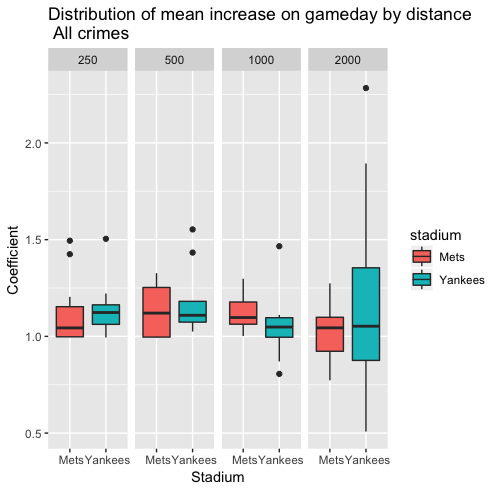
\includegraphics[scale=0.5]{box_4.png}
\end{figure}

Analyzing  the second graph there is are slightly evident differences between the two stadiums. The main one, is that the variance of the increase in crimes is much bigger for the crimes 20000 meters around Yankee's stadium, although there is no difference with respect to the mean. The mean increase in crimes is higher for Yankee stadium on the 200 meter vicinity , while it is higher for the mets stadium if we consider the 1000 meter vicinity. 

Even though  the last analyses showed some differences, analyzing this result in a crime segmentation instead of a distance segmentation could show specific differences. The next graph shows the box plot distributions per crime, it is summarizing over different vicinity sizes. It is important to remember that this are the crimes whose estimated $\beta$ coefficient was significant for all four vicinity sizes.  

\begin{figure}[H]
\centering
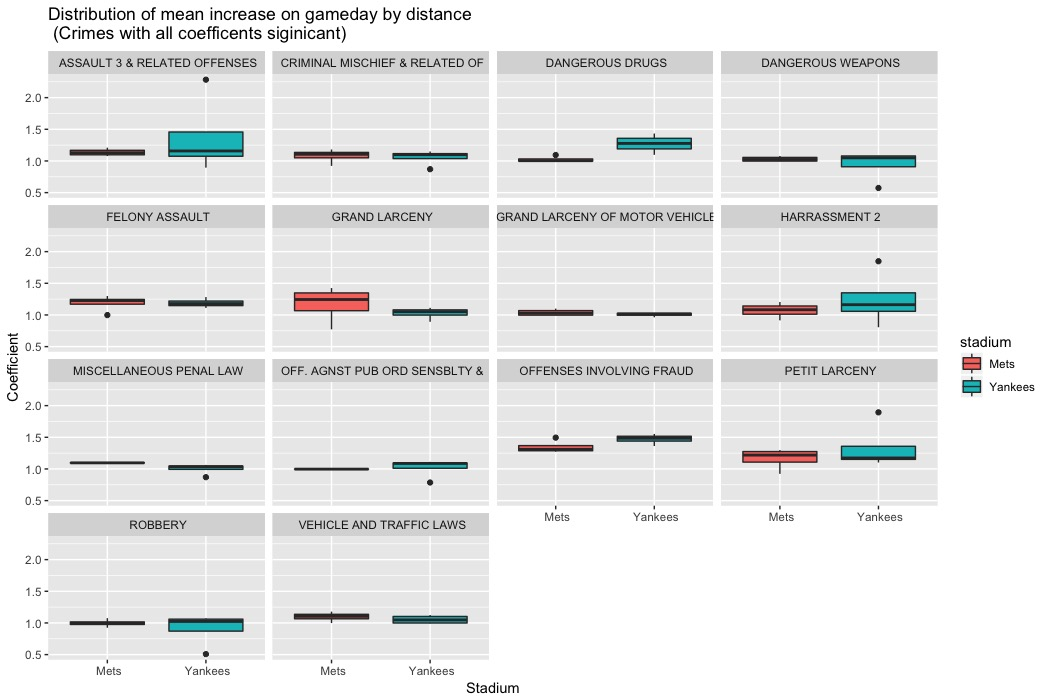
\includegraphics[scale=0.45]{box_plot_means.jpeg}
\end{figure}

From this plot  it is clear that for some crimes there is basically no  difference. Examples of crime increase with no difference between stadiums: "Criminal mischief", "Grand larceny of motor vehicle", "Felony assault", and "Vehicle and traffic laws". On the contrary, for some crimes it is clear that the increase is different between stadiums. From the significant selection, "Grand larceny" is the only crime that increases more around Mets Stadium than it does around Yankees stadium. On the other hand, the crimes "Assault \& related", "Dangerous drugs", "Harassment", and "Offenses involving fraud" clearly increase more in the vicinity around Yankee stadium.  In general, the crime increase around Yankee stadium show a higher variance among vicinity sizes , while the increase of crime around the Mets stadium  is more constant for the different vicinity sizes.

To finalize this analysis, the following graphs shows a one-on-one comparison of the estimated coefficients for all the vicinity sizes and crimes. 

\begin{figure}[H]
\centering
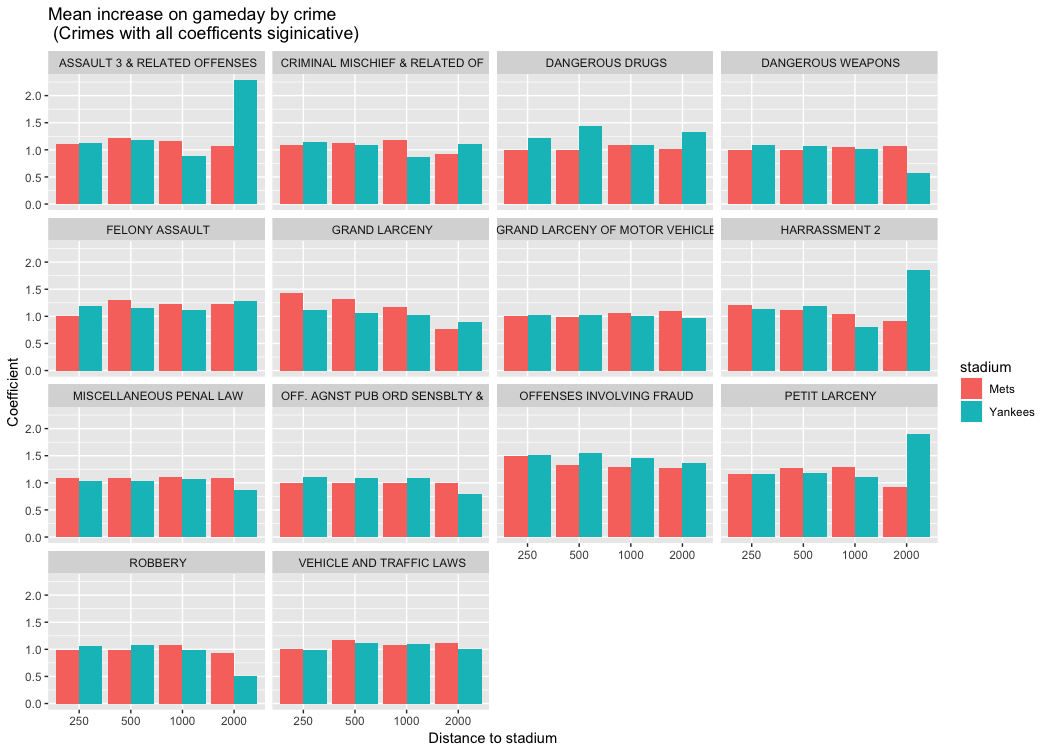
\includegraphics[scale=0.45]{mean_increase.png}
\end{figure}

These plots show that the crime increase around stadiums is mainly the same. Differences mainly occur in the 2000 meter vicinity. For three crimes, the crime increase around Yankee stadium  is clearly higher.  It is important to note that Yankee stadium is closer to the most densely populated area of New York City, therefore, different factors need to be considered when comparing results for the 2000 meter vicinity. 

A complementary approach is to evaluate the $\beta$ parameter as a percentage increase with respect to $\alpha$. Although the last analysis was done over data of the same magnitude, different results could show up if we study the increase in crime during Game-day as a percentage increase over any day. The next plots are the replica of the past analysis, this time using mean percentage increase.

\begin{figure}[H]
\centering
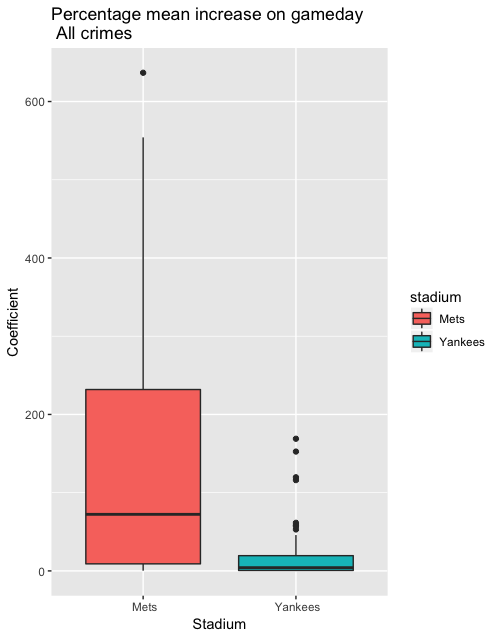
\includegraphics[scale=0.45]{percent_box_1.png}
\end{figure}

From this second approach, there is a clear difference between the percent increase in crime between stadiums. While the mean of percent increase is close to zero for the Yankee's stadium, it is about 70\% for the Mets stadium. Considering that the absolute results were very similar, this is a huge difference.  The box that includes 50\% of the observations has an upper bound above 200\% therefore some crimes are three times more common  during Game-day at the Mets Stadium vicinity. 

The next plots show the  distribution of  percent crime increase for each vicinity size. This graph should let us know what is the relationship between the crime increase and the distance to the stadium.

\begin{figure}[H]
\centering
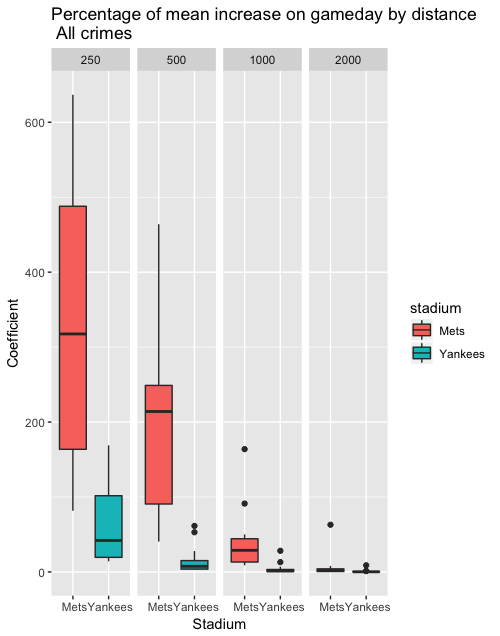
\includegraphics[scale=0.45]{percent_box_4.png}
\end{figure}

This graph clearly shows that the percent crime increase is higher in the closer areas to the stadiums. For the 200 meter vicinity around Met's stadium, the mean percent crime increase is above 300\% and the upper bound of the box is very close to 500\%. As the vicinity size increases, the distribution of percent crime increase during Game-day decreases until reaching a level close to zero for the 2000 meter vicinity. The pattern is similar for the vicinities around Yankee's stadium, but in a lower scale. Again, it is very clear that crime increase in percent is greater in the Met's Stadium vicinity, at least up to the 1000 meter vicinity.

The next step is to evaluate the percent increase per crime over all the vicinities. The next plot allows to make the analysis for the crimes with significant coefficients .

\begin{figure}[H]
\centering
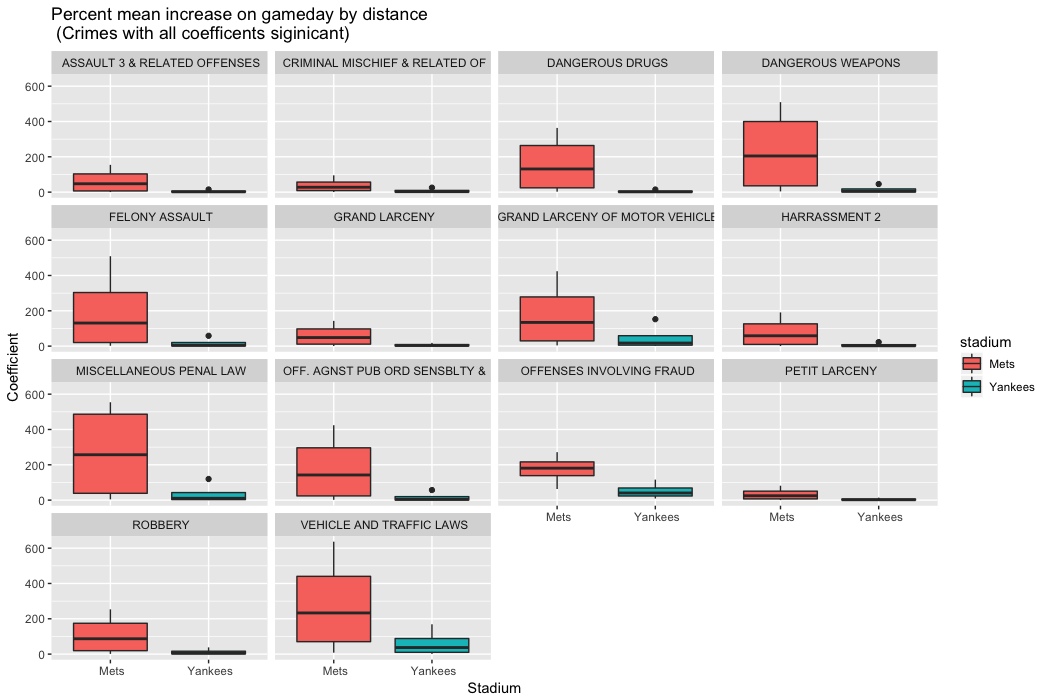
\includegraphics[scale=0.45]{percent_all_boxes.png}
\end{figure}

As expected the crime increase in percent is much higher  at the Met's stadium vicinity for most crimes. The crimes with a  clear difference are: "Dangerous drugs", "Dangerous Weapons", "Felony assault", "Grand larceny  of motor vehicle", "Harassment" , "Miscellaneous penal law", "Offenses involving fraud", "Robbery", and "Vehicle traffic laws". For the rest of crimes, the  percent increase is also larger at the Met's stadium vicinity in a smaller degree.

Finally we also show the plot with the one on one comparison of the  coefficients representing percent crime increase. This graph evidences details that are not visible when working with aggregated data.


\begin{figure}[H]
\centering
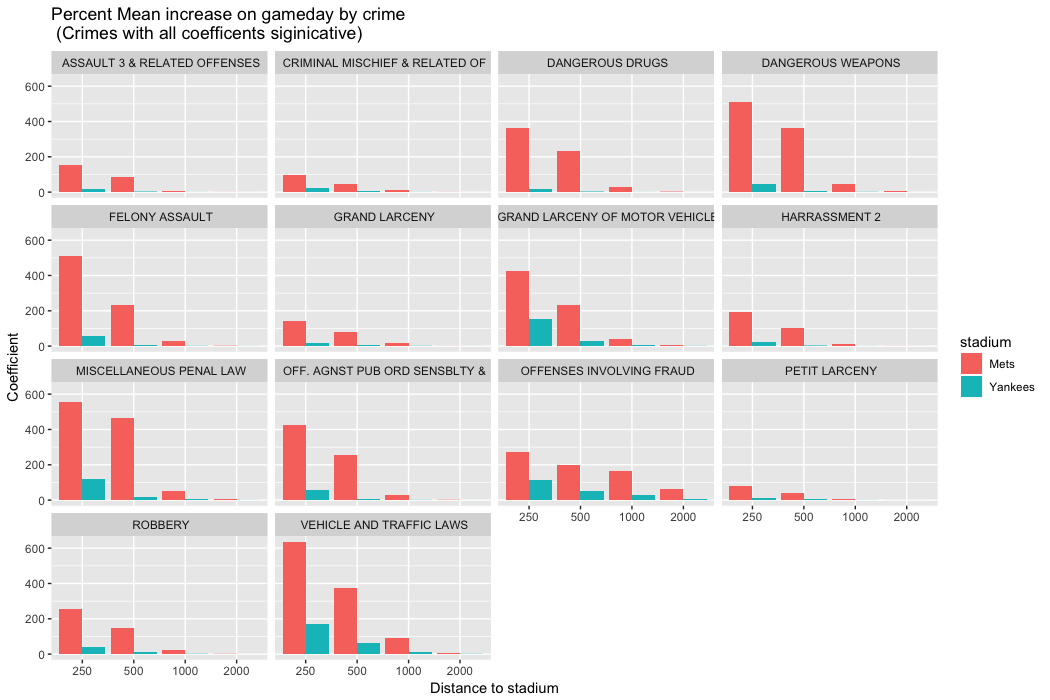
\includegraphics[scale=0.45]{percent_bars.png}
\end{figure}

This graph clearly shows that the percent increase for all crimes is higher around the Met's Stadium. It also shows the rate of increase is much higher for the smaller vicinity  we consider. In general, although the increase of crime is evident around both stadiums, the percent increase  of crime is much higher around Mets Stadium.

\subsubsection{Discussion}

First, it is important to note the difference of the results from both approaches. When considering the absolute increase in crime (first approach), there where not a lot of evident differences.  Although the coefficients are very similar, it seemed that the increase was higher around Yankee's stadium, at least for the 2000 meter vicinity. When studying the percent increase in crime, our fitted models showed a completely different story. For all crimes, the percent increase in much higher around the Mets stadium. We further discuss why we might see these results.

An important result to note is that for both stadiums, the percent increase in crime is larger the smaller vicinity size  we choose. The results show clear increase of crime up to 1000 meters around the stadiums. When considering crime increase in the  2000 meter vicinity the percent a is very small, therefore we can conclude that a Game-day is not so influential once you consider  vicinities over 2000 meters.  A more detailed could be done to find a more accurate threshold, i.e. a distance between 1000 and 2000 meters.

Additionally, we have to consider that this analysis is not accounting for population density. The area around Yankee stadium is more densely populated than the area around the Met's Stadium. Possibly, if we adjust the analysis to account for this factor we could find different results, either making the percent increase similar for both stadiums vicinities or accentuating the difference.


\pagebreak
\section{Summary and Conclusions}

In this project we addressed the quality of the Crime data provided  by the City of New York. We worked with more than 5.58 million instances and 24 variables. Initially, we described the temporality of data, finding issues on the year and time of occurrence. We concluded that we could only use data from 2006 onwards. Besides that there were only minor issues in the data.   

For the analysis section, we evaluated 6 different hypothesis in two main topics: Sociodemographic characteristics of population and Baseball Games. For the first topic we used the spark ML library to calculate correlation coefficients between crime occurrences and total population, population under poverty level, black population, and under-educated population. The data was aggregated by year and borough to build comparable variables. Every borough had at least 3 out 4 features to be directly positively correlated with the crime rate. This also explains why the Pearson correlation rate was so high. We conclude that that higher population, higher black population as percent of total population, higher population below poverty line and lower educated population as percentage of total population is highly correlated with an increase in crime at any given Borough in any given year.  

Regarding the second topic, we concluded that crime increases on Baseball Game-day near the stadium in that particular day. To build this result we fitted over 500 linear regressions for different crimes, stadiums and vicinity sizes using the pyspark ML library. Given the novelty of the library and the absence of documentation in forums, we had to settle with this simple model. The estimated coefficients that indicated if it was a game are positive values for all the significant models, therefore, we are certain that a Game-day is related with an increase in crime. 

As a more detailed study of this second topic , we compared the crime increase between stadiums using the regression outputs. First we compared the absolute crime increase, finding very little differences. Then we compared the relative crime increase, finding a larger percent crime increase at the Citi Field vicinity. We conclude that the relative crime increase during Game-day is clearly larger around the Met's stadium vicinity for most of the crimes, we also  found that a 2000 meter vicinity is too large to study the effect of Game-day. Additionally, we believe a further analysis could scale the crime increase according to population density to find results relative to the population increase in the area. 

We should also consider that some "crimes" in our analysis involve traffic incidents, not crimes but accidents. It is important to note this because when there is a large amount of people and cars moving towards the same point, a Baseball stadium for example, there is an expected amount of accidents. Therefore, some observations should not be considered crimes threat a person's security, but inevitable accidents that are naturally part of a Baseball game. 

One of the main weakness of this analysis, is that it considers the data to be generated randomly: the Baseball Games are distributed randomly over the days of a year, and so are the crimes. This is obviously not the case, and it is easy to think on another hypothesis that may be driving all these results up: Baseball games are on the spring and summer, more people go out to the streets on spring and summer compared to winter and autumn, so there are more crimes on just because the people go out more. 

In general we can say that the crime  occurrence is strongly correlated with the population density. This was shown in the first hypothesis and confirmed on the second one, considering that a Game-day accounts for a temporary population increase. 

\pagebreak
\section{Individual Contributions}

We believe that \textbf{all the member of the team participated equally in the generation of this report, and all the members generated and analyzed at least some part of the data using the tools seen in class}, specifically pyspark. While some members performed more data-crunching wile others performed more data-analysis, all of us believe the work load was evenly distributed among all members, making sure all of us worked our pyspark skills. 

Particularly, Raúl generated the code to analyze the data using sparkSQL, and help building some of the functions on the Baseball hypothesis building, plus analyzed the Mets VS Yankees hypothesis. 

Akash was responsible for the sociodemographic hypothesis, including the pyspsark and SQL data analysis, and helped providing insights in the data-analysis section.

Finally, Eduardo was responsible for scrapping the Baseball data and developing the code to run all the regressions on pyspark (alongside Raul). He also provided the detailed analysis and graphs on for the data quality section, including the pyspark code to generate the crunched data.  

We all worked in the write up, specially in the sections we were in charge.

\newpage
\printbibliography 
\end{document}